\documentclass[12pt, a4paper]{article}

% --- Packages ---
\usepackage[margin=1in]{geometry}
\usepackage{graphicx}
\usepackage{hyperref}
\usepackage{xcolor}
\usepackage{booktabs}
\usepackage{enumitem}
\usepackage{titlesec}
\usepackage{fancyhdr}
\usepackage{tabularx}
\usepackage{float}
\usepackage{caption}
\usepackage{subcaption}
\usepackage{tcolorbox}
\usepackage{parskip}
\usepackage{array}
\usepackage{longtable}
\usepackage{multirow}

% --- Subtle border around images ---
\setlength{\fboxsep}{0pt}
\setlength{\fboxrule}{0.3pt}
\newcommand{\imgborder}[1]{\fcolorbox{gray!40}{white}{#1}}

% --- Colors ---
\definecolor{primary}{HTML}{2A348C}
\definecolor{accent}{HTML}{14BEF0}
\definecolor{violation}{HTML}{DC2626}
\definecolor{solution}{HTML}{059669}
\definecolor{hciconcept}{HTML}{7C3AED}
\definecolor{endsemblue}{HTML}{1D4ED8}
\definecolor{midsemdark}{HTML}{374151}

% --- Hyperlink setup ---
\hypersetup{
    colorlinks=true,
    linkcolor=primary,
    urlcolor=primary,
    citecolor=primary
}

% --- Section formatting ---
\titleformat{\section}{\Large\bfseries\color{primary}}{}{0em}{}[\titlerule]
\titleformat{\subsection}{\large\bfseries\color{primary!80!black}}{}{0em}{}
\titleformat{\subsubsection}{\normalsize\bfseries\color{hciconcept}}{}{0em}{}

% --- Header/Footer ---
\pagestyle{fancy}
\fancyhf{}
\rhead{\textcolor{gray}{ME23B1004}}
\lhead{\textcolor{gray}{CS5015 --- HCI End Sem Design Activity}}
\cfoot{\thepage}

% --- Custom tcolorbox environments (same as midsem) ---
\newtcolorbox{violationbox}{
    colback=violation!5, colframe=violation!60!black,
    title={\textbf{Violation Identified in Practo}},
    fonttitle=\bfseries\color{white}, coltitle=white,
    colbacktitle=violation!80!black, sharp corners=south
}

\newtcolorbox{solutionbox}{
    colback=solution!5, colframe=solution!60!black,
    title={\textbf{My Solution in Better Practo}},
    fonttitle=\bfseries\color{white}, coltitle=white,
    colbacktitle=solution!80!black, sharp corners=south
}

\newtcolorbox{hcibox}[1]{
    colback=hciconcept!5, colframe=hciconcept!50!black,
    title={\textbf{HCI Concepts Applied: } #1},
    fonttitle=\bfseries\color{white}, coltitle=white,
    colbacktitle=hciconcept!70!black, sharp corners=south
}

% New box for end-sem feature blocks
\newtcolorbox{featurebox}[1]{
    colback=endsemblue!4, colframe=endsemblue!50!black,
    title={\textbf{End-Sem Feature: } #1},
    fonttitle=\bfseries\color{white}, coltitle=white,
    colbacktitle=endsemblue!80!black, sharp corners=south
}

% ================================================================
\begin{document}

% =================================================================
%  COVER PAGE
% =================================================================
\begin{titlepage}
\centering
\vspace*{2cm}

{\Huge\bfseries\color{primary} End Sem --- Design Activity}\\[0.8cm]
{\LARGE\color{primary!70!black} Human Computer Interaction}\\[0.3cm]
{\large Course Code: CS5015}

\vspace{1.5cm}

\rule{\textwidth}{1pt}
\vspace{0.5cm}

{\Large\bfseries Domain: Online Doctor Consultation App}\\[0.3cm]
{\large (Better Practo --- Enhancement of Mid-Sem Design)}\\[0.2cm]
{\large\url{https://www.practo.com}}

\vspace{0.5cm}
\rule{\textwidth}{1pt}

\vspace{2cm}

{\Large\bfseries R. Abinav}\\[0.3cm]
{\large Roll No: \textbf{ME23B1004}}

\vspace{2cm}

\vfill
{\small April 2026}
\end{titlepage}

% =================================================================
%  TABLE OF CONTENTS
% =================================================================
\tableofcontents
\newpage

% =================================================================
\section{Introduction}
% =================================================================

This report is the \textbf{End-Semester Design Activity} for CS5015 --- Human Computer Interaction. It extends the mid-semester ``Better Practo'' project by applying advanced HCI concepts taught in the second half of the course (Lectures 9--15+).

\textbf{The mid-semester submission} identified \textbf{14 usability violations} in \href{https://www.practo.com}{Practo.com} and fixed each one in a React + Tailwind CSS prototype. That work covered: Shneiderman's 8 Golden Rules, Nielsen's 10 Heuristics, Miller's 7$\pm$2, Hick's Law, Fitts's Law, Inverted Pyramid, Closure, F-Pattern, Learnability, Power Law, Asimov's Laws, Zipf's Law, and the Password Masking case study.

\textbf{This end-semester submission} layers the following post-mid-sem concepts on top of that foundation:

\begin{itemize}[leftmargin=1.5em]
  \item \textbf{Block A} --- Gestalt Laws (Proximity, Similarity, Figure \& Ground, Continuity, Common Fate, Closure)
  \item \textbf{Block B} --- Visual Design (Dominance, Scale, Balance, Hierarchy, Contrast, Negative Space)
  \item \textbf{Block C} --- Persuasion Psychology (Cialdini's 6 Principles)
  \item \textbf{Block D} --- Color \& Shape Psychology
  \item \textbf{Block E} --- User Support Systems (Quick Reference, Context-Sensitive Help, Assistants)
  \item \textbf{Block F} --- Navigation Design (Skip Links, Breadcrumbs, Keyboard Focus)
  \item \textbf{Block G} --- Interaction Design Paradigms (Direct Manipulation, Menu Selection, Form Fill-in)
  \item \textbf{Block H} --- Web Usability Guidelines (Krug's Don't Make Me Think, Feature Exposure, 404)
  \item \textbf{Block I} --- Universal Design (7 Principles, WCAG accessibility)
  \item \textbf{Block J} --- Google Search Case Study (Explorer vs Navigator Users)
  \item \textbf{Block K} --- CAPTCHA Design Principles
  \item \textbf{Block L} --- Enhanced Mid-Sem Features (framer-motion, 4th onboarding step)
\end{itemize}

\textbf{Tech Stack:} React 18 + Tailwind CSS 3 + Vite 6 + Framer-Motion + Lucide-React.

\vspace{0.5cm}

% =================================================================
\section{Block A --- Gestalt Laws}
% =================================================================

\begin{hcibox}{Gestalt Laws of Perceptual Organization}
Gestalt psychology (Wertheimer, 1923) describes how the human brain groups visual stimuli into unified wholes. The six laws applied here are: \textbf{Proximity} (nearby elements appear grouped), \textbf{Similarity} (identical style = same category), \textbf{Figure \& Ground} (one region is perceived as the figure, another as background), \textbf{Continuity} (the eye follows smooth paths), \textbf{Common Fate} (elements moving together are perceived as a group), and \textbf{Closure} (incomplete shapes are completed by the brain).

\textit{Reference: End-Sem HCI Lecture Notes, lines 4--17.}
\end{hcibox}

\vspace{0.4cm}

The \textbf{Find Doctors} (Search) page was redesigned to demonstrate all six Gestalt laws simultaneously.

\subsection{A1 --- Gestalt Proximity \& Similarity}

\begin{featurebox}{Gestalt Proximity + Similarity on Doctor Cards}
\textbf{Proximity:} Within each doctor card, the name/specialty/experience cluster is separated from the availability/location cluster with explicit vertical spacing (\texttt{mt-3} gap), creating two visually distinct groups. Users do not need to read every element --- the grouping communicates structure pre-attentively.

\textbf{Similarity:} All ``Verified'' badges use \emph{identical} JSX and styling (\texttt{bg-accent-100}, check-circle icon, rounded-full). All ``Available Today'' pills use identical green styling; all ``Available Tomorrow'' pills use identical amber styling. This ensures that similar visual form signals the same semantic meaning across all cards --- users recognise the pattern after seeing it once.
\end{featurebox}

\subsection{A2 --- Gestalt Figure \& Ground + Continuity}

\begin{featurebox}{Gestalt Figure \& Ground + Continuity}
\textbf{Figure \& Ground:} The page background is \texttt{bg-trust-50} (light slate grey), while each doctor card is \texttt{bg-white}. The white cards ``pop'' as the figure against the grey ground, creating a clear separation without borders or shadows alone.

\textbf{Continuity:} A subtle left-border stripe (\texttt{border-l-2 border-primary-100 pl-3}) runs down the metadata section of each card (availability badge, location), guiding the user's eye downward through the information hierarchy in a single smooth column --- exactly as the eye naturally follows continuous lines.
\end{featurebox}

\subsection{A3 --- Gestalt Common Fate (Sort Animation)}

\begin{featurebox}{Gestalt Common Fate --- framer-motion AnimatePresence}
When the user clicks a sort pill (e.g.\ ``Rating'' or ``Experience''), all doctor cards animate in the \emph{same direction simultaneously} (\texttt{y: 0} from \texttt{y: 20}). This simultaneous motion causes the brain --- per the Common Fate law --- to perceive all cards as a single unified group, not 96 independent elements. This also reinforces the Direct Manipulation principle (Block G): the effect of the sort is instantly and visibly perceived rather than happening silently.

\textit{Implementation: \texttt{framer-motion} \texttt{<AnimatePresence mode="popLayout">} wraps the results list. Each card is a \texttt{<motion.div>} with \texttt{layout}, \texttt{initial=\{opacity:0, y:20\}}, \texttt{animate=\{opacity:1, y:0\}}, \texttt{exit=\{opacity:0, y:-20\}}, \texttt{transition=\{duration: 0.22\}}.}
\end{featurebox}

\subsection{A4 --- Gestalt Closure}

\begin{featurebox}{Gestalt Closure --- Progress Indicator on Booking Page}
Closure: The brain completes incomplete figures. The 3-step progress indicator on the Booking page (implemented in the mid-semester) uses partially filled circles for incomplete steps. Even though the circle is not drawn completely, the user's perceptual system automatically ``closes'' it and understands the concept of ``step not yet complete vs step done.'' This requires zero explanation.
\end{featurebox}

\vspace{0.3cm}

\begin{figure}[H]
    \centering
    \imgborder{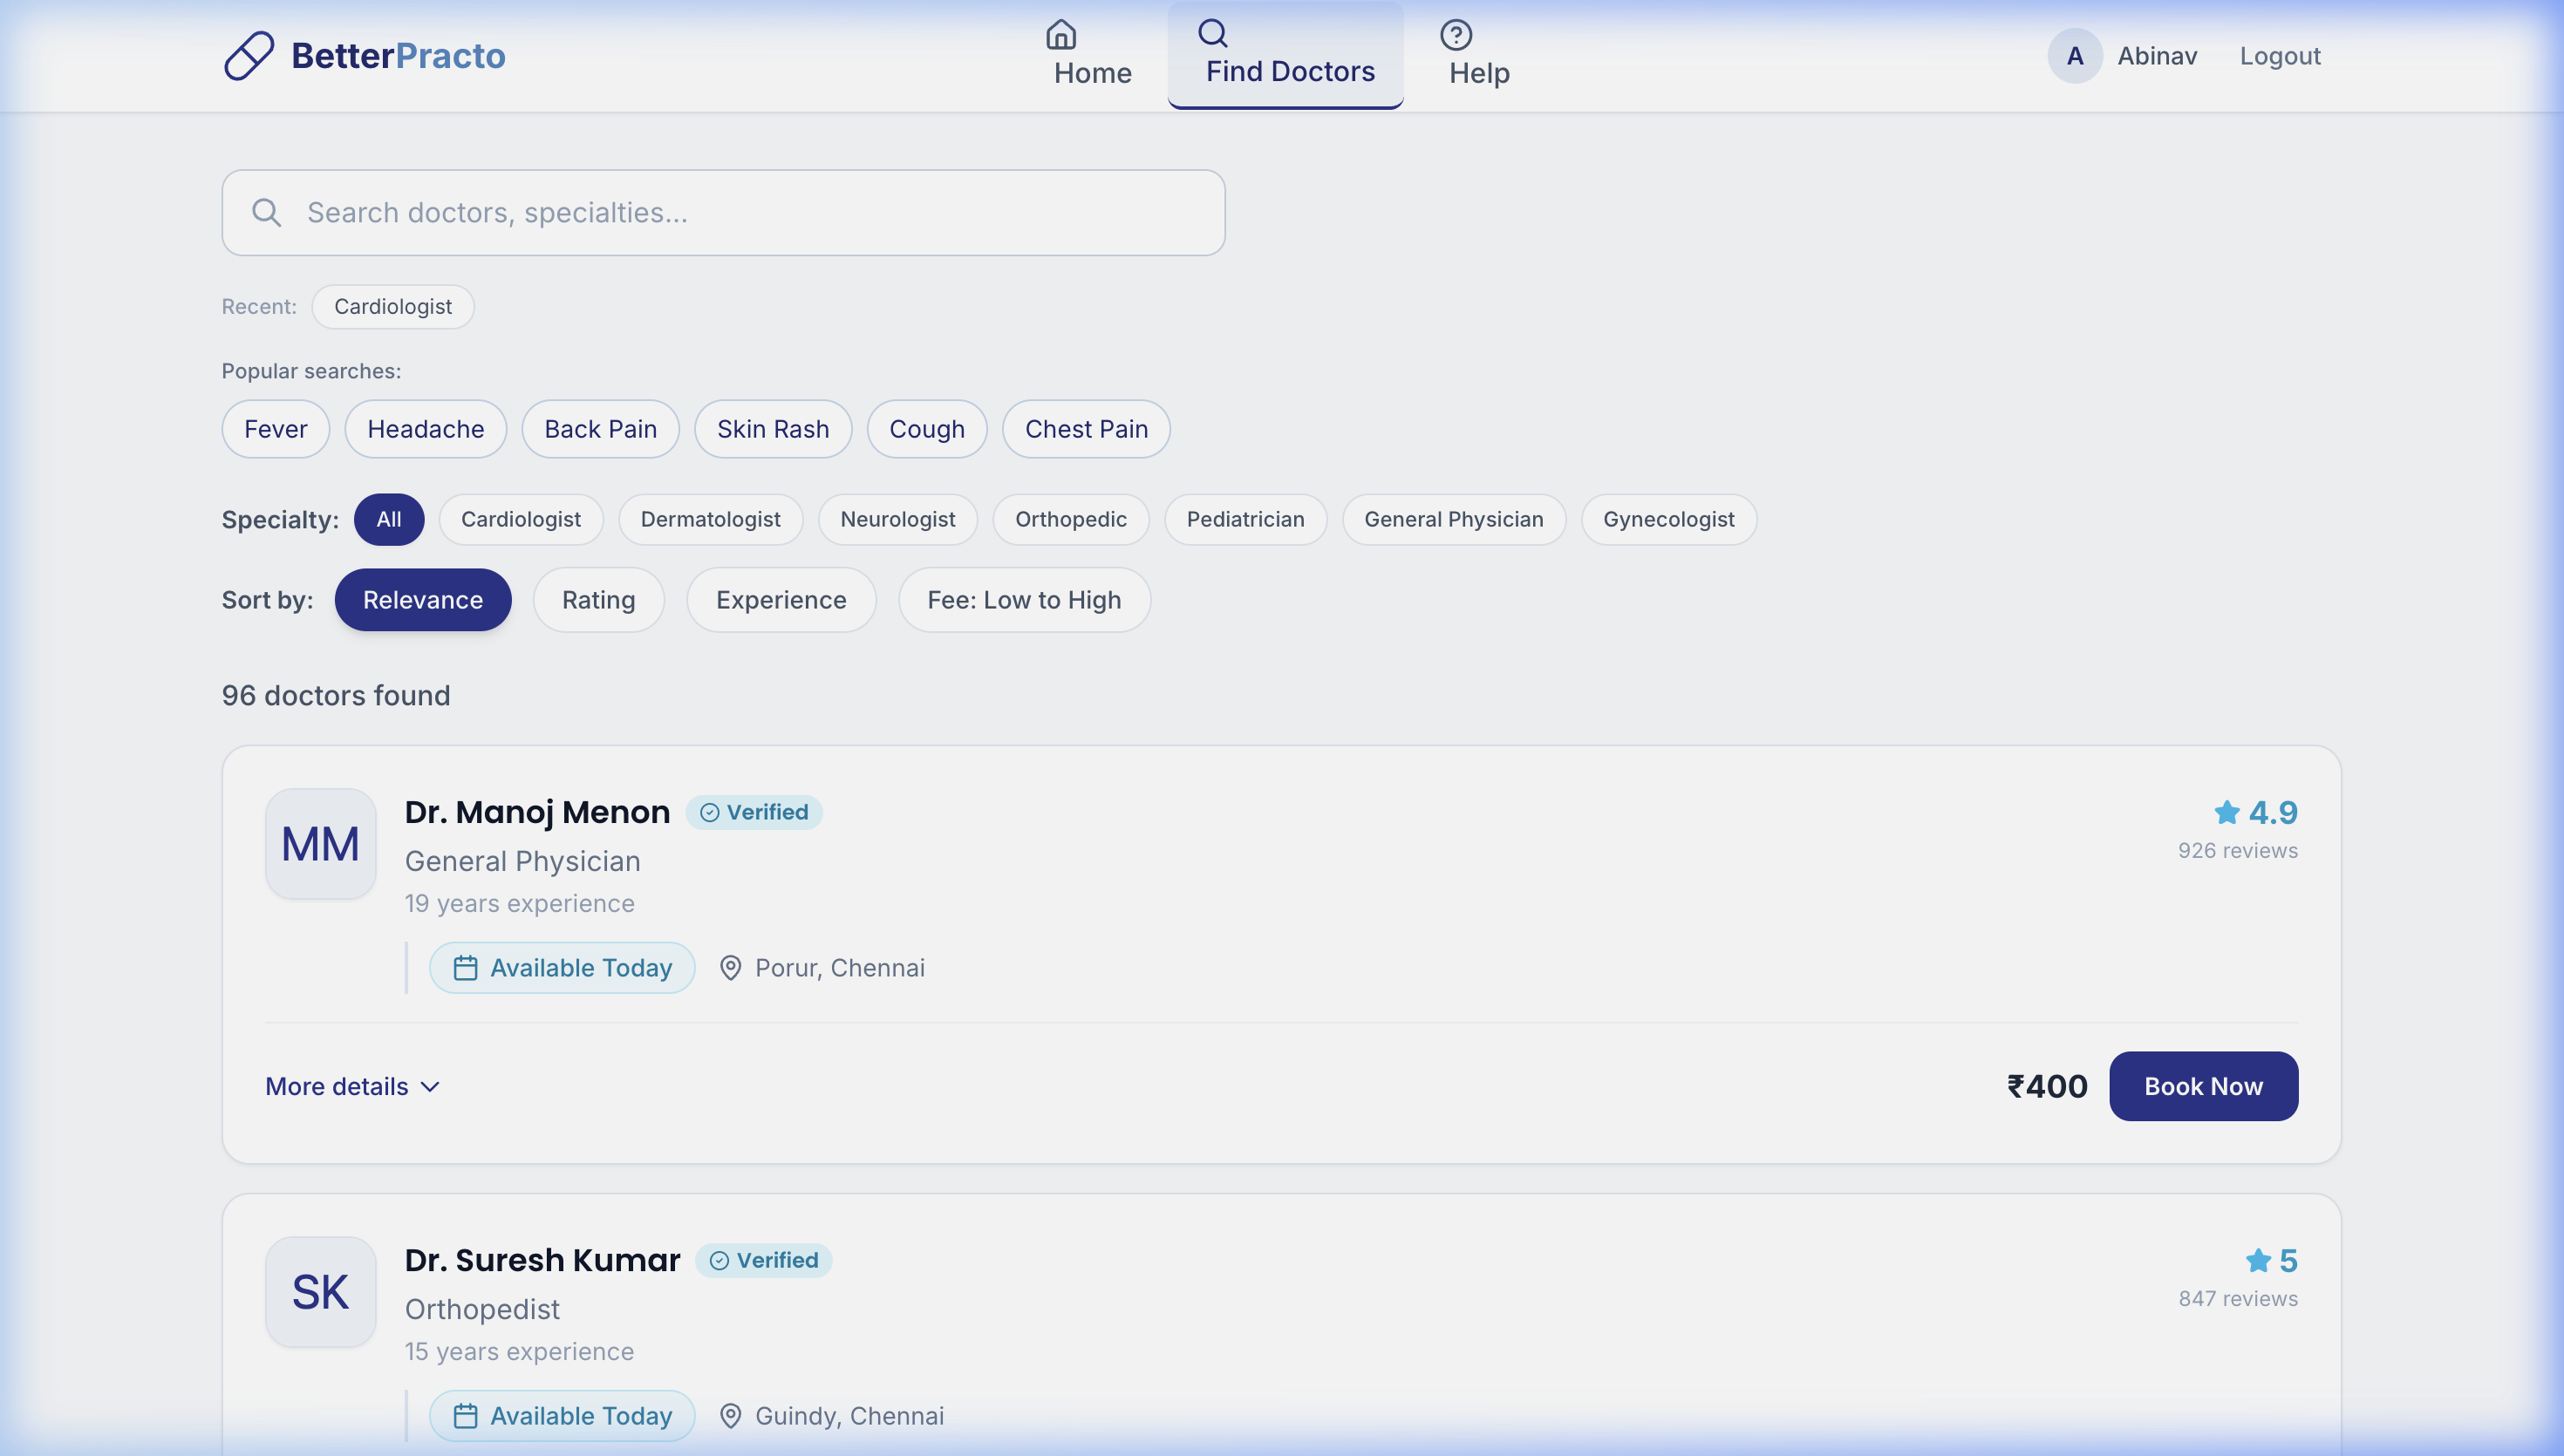
\includegraphics[width=\textwidth]{gestalt_search_cards.png}}
    \caption{Search page showing Gestalt Proximity (grouped clusters), Similarity (identical badge styles), Figure \& Ground (white cards on grey background), and Continuity (left-border stripe). \textit{Block A.}}
\end{figure}

\begin{figure}[H]
    \centering
    \imgborder{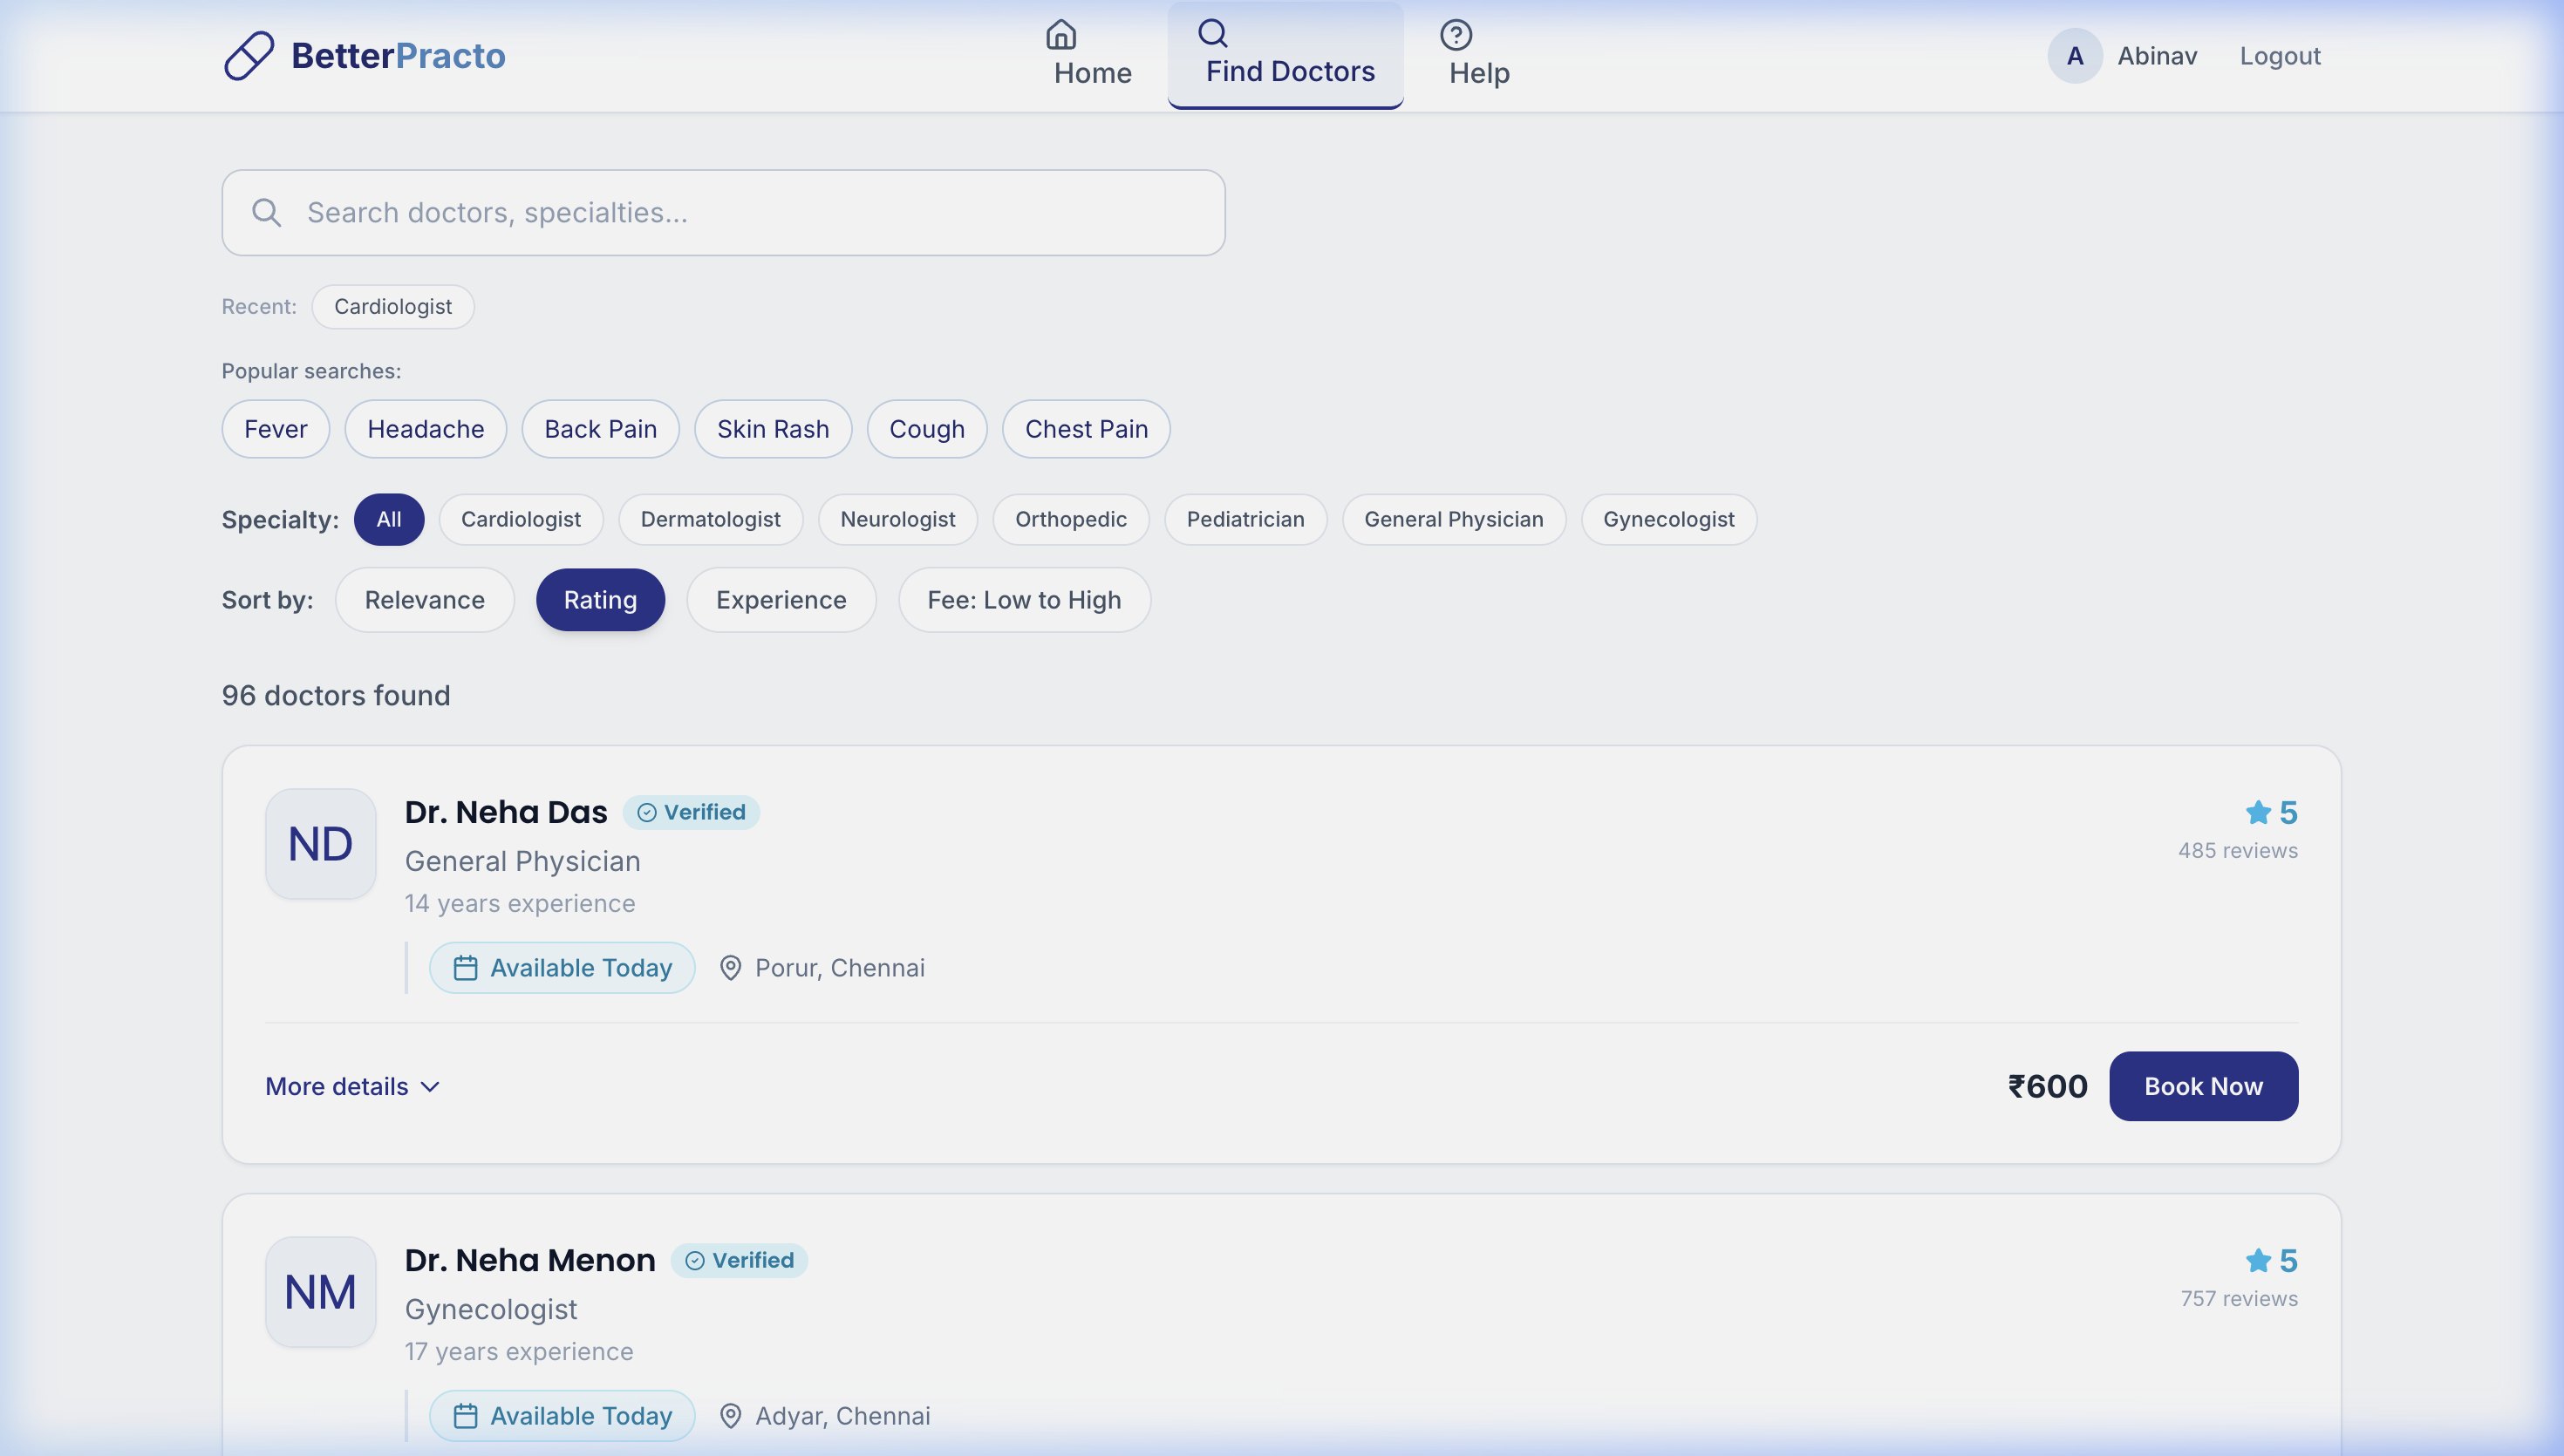
\includegraphics[width=\textwidth]{gestalt_sort_animation.png}}
    \caption{After clicking the ``Rating'' sort pill --- all cards animate together (Common Fate law). The simultaneous motion signals to the brain that these elements form a unified group. \textit{Block A.}}
\end{figure}

\vspace{0.5cm}

% =================================================================
\section{Block G --- Interaction Design Paradigms}
% =================================================================

\begin{hcibox}{Interaction Design Paradigms}
Foley \& van Dam (1990) classify human--computer interaction into four fundamental paradigms: \textbf{Command Language} (user types commands --- expert, powerful, steep learning curve), \textbf{Form Fill-in} (user completes structured fields --- familiar, error-prone if unlabelled), \textbf{Menu Selection} (user picks from a predefined set --- discoverable, low cognitive load), and \textbf{Direct Manipulation} (objects acted on immediately; results visible instantly; actions easily reversible --- Shneiderman, 1982).

\textit{Reference: End-Sem HCI Lecture Notes, lines 234--295.}
\end{hcibox}

\subsection{G1 --- Menu Selection: Specialty Filter Pills}

\begin{featurebox}{Menu Selection --- Specialty Filter Row}
Above the sort pills on the Search page, a row of specialty filter pills (All, Cardiologist, Dermatologist, Neurologist, Orthopedic, Pediatrician, General Physician, Gynecologist) implements the \textbf{Menu Selection paradigm}. The user picks from a bounded, visible set of options without typing. Benefits: discoverable (options are always visible), low error rate (no typos possible), and fast for both novice and expert users. This contrasts with a \textbf{Command Language} approach where the user would have to type the exact specialty name.
\end{featurebox}

\subsection{G2 --- Direct Manipulation: Sort Pills + Card Animation}

\begin{featurebox}{Direct Manipulation --- WYSIWYG Sort}
Clicking a sort pill is a textbook \textbf{Direct Manipulation} interaction: (1) the object of interest (the card list) is continuously represented, (2) the action (clicking ``Rating'') is physical and immediate, (3) results are visible instantly via the framer-motion animation (Common Fate, Block A), and (4) the action is easily reversible (click ``Relevance'' to undo). This satisfies all four of Shneiderman's criteria for direct manipulation. Slot selection in the Booking page Step 1 uses the same principle --- selected slots animate with \texttt{whileTap} scale feedback.
\end{featurebox}

\begin{figure}[H]
    \centering
    \imgborder{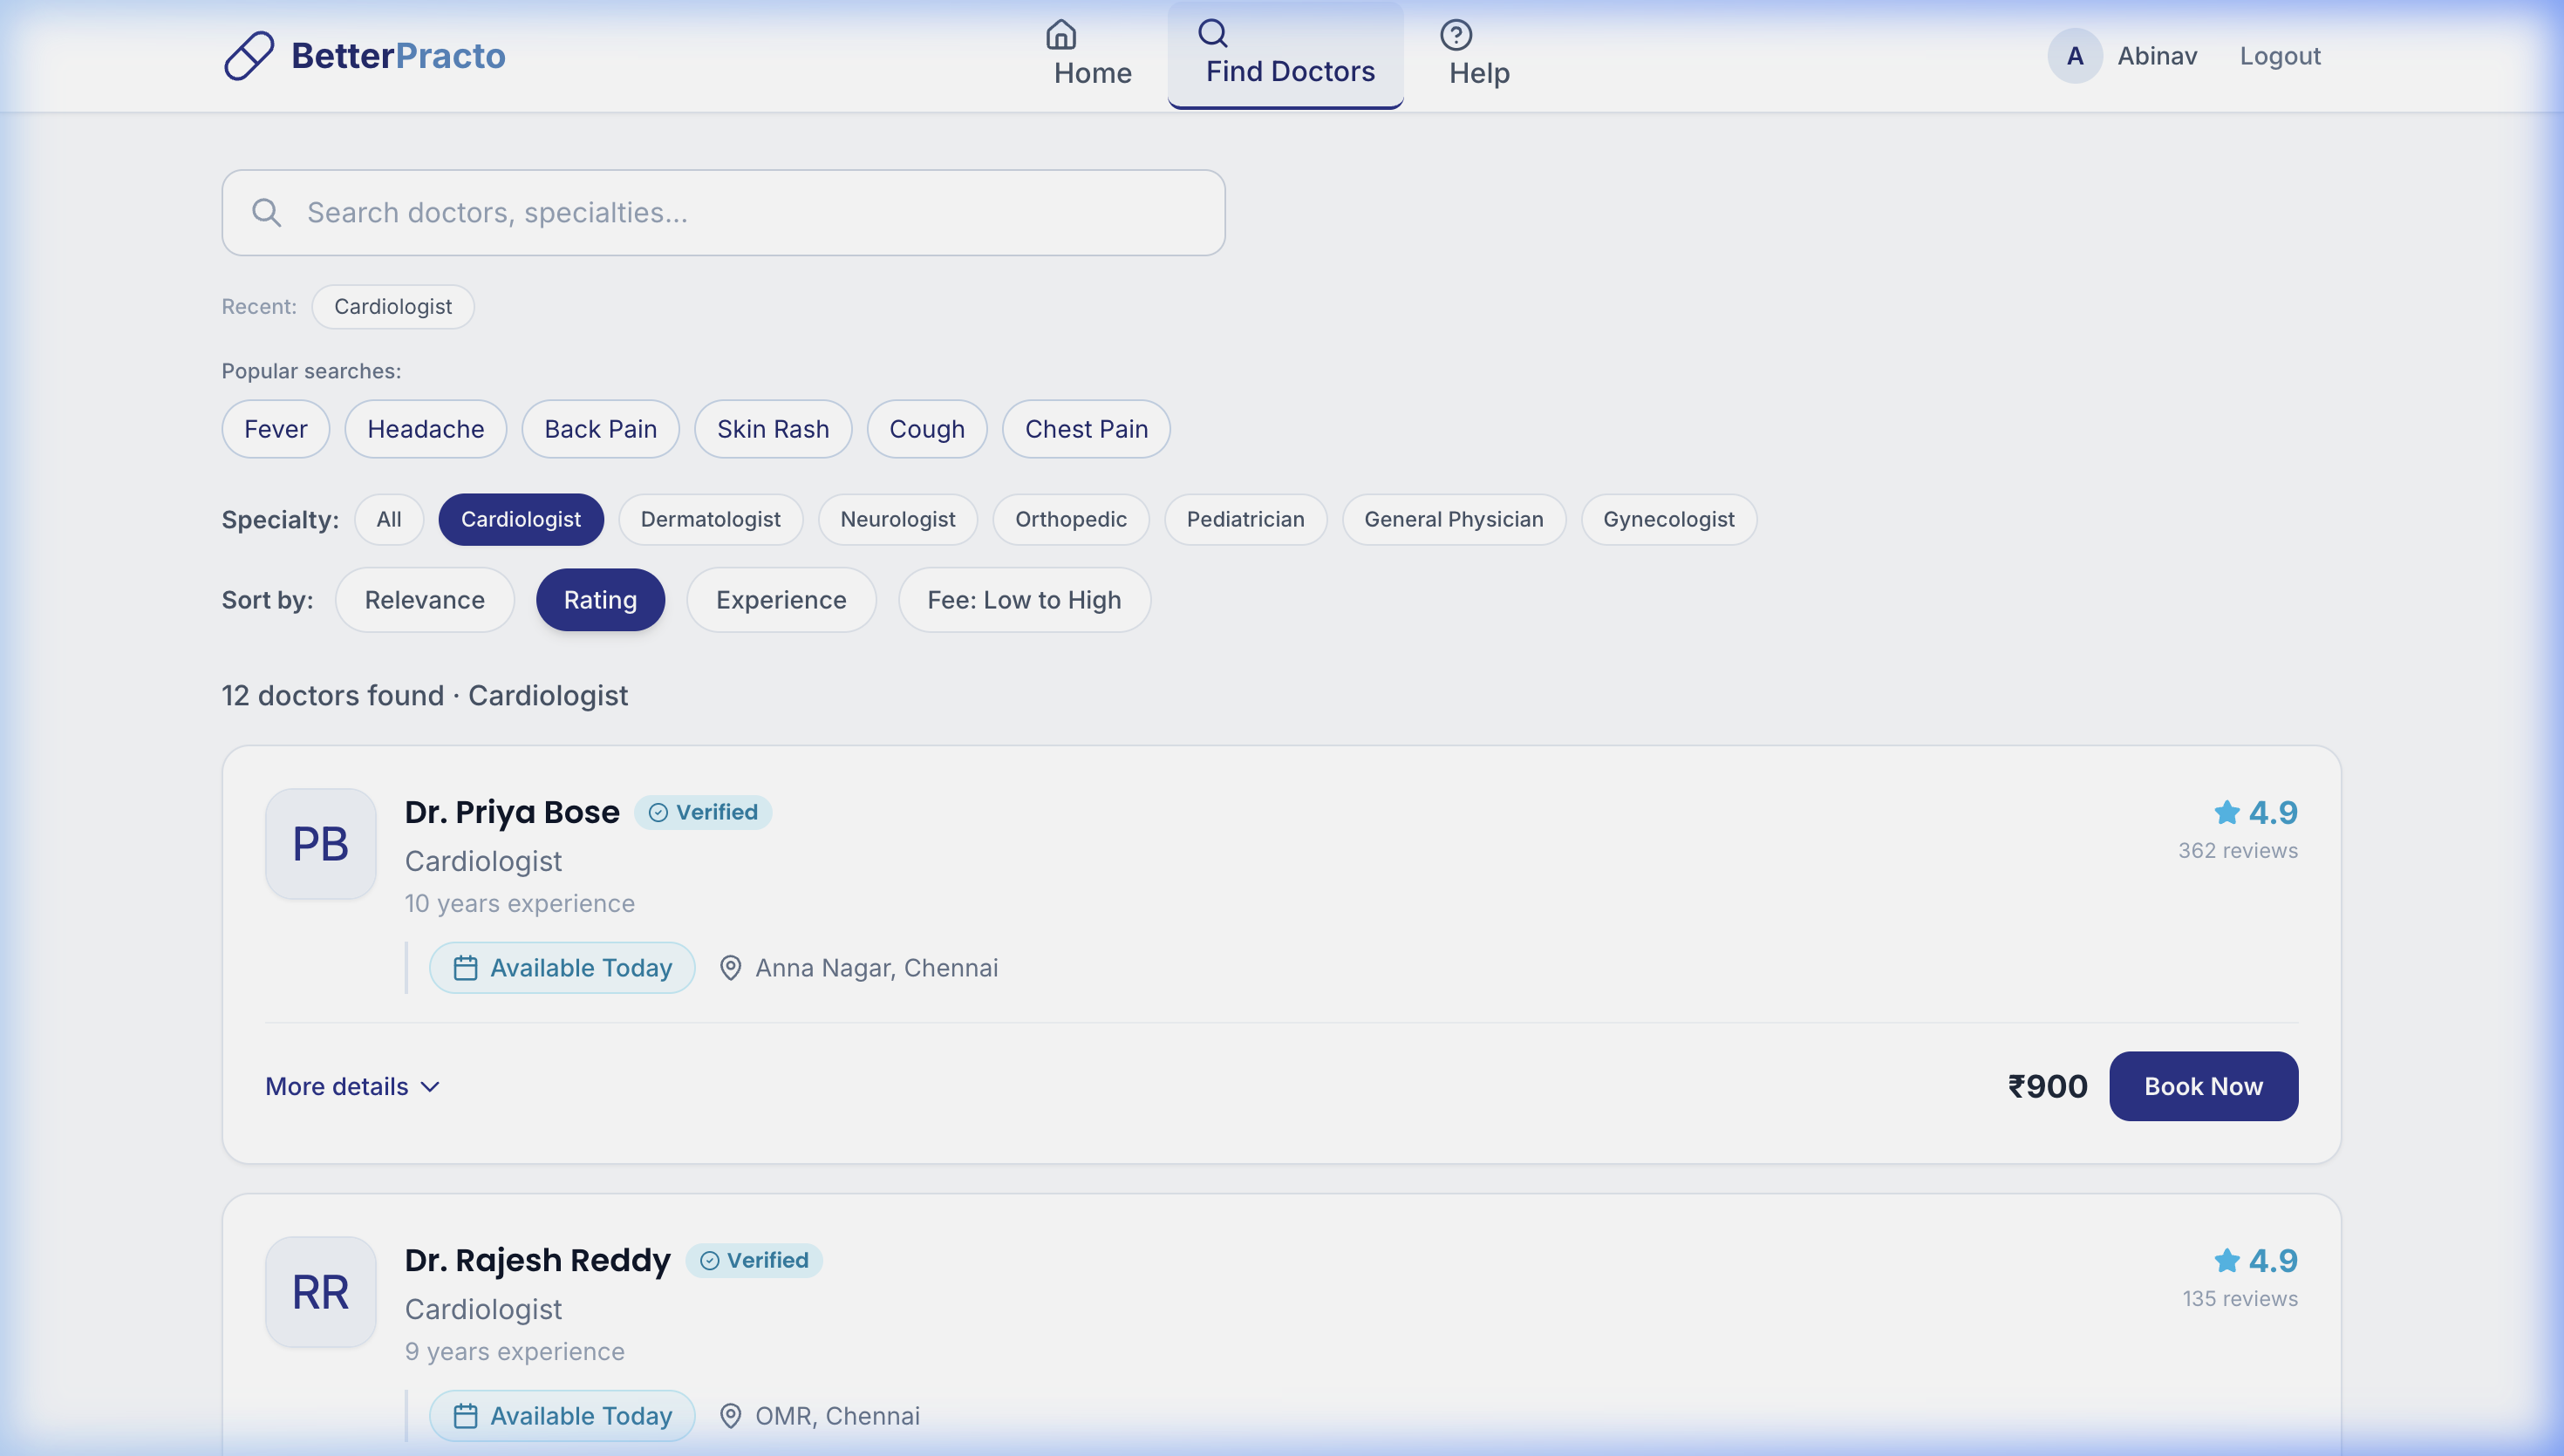
\includegraphics[width=\textwidth]{interaction_menu_filter.png}}
    \caption{``Cardiologist'' specialty pill selected (Menu Selection paradigm). Only cardiologists appear --- no typing required. The active pill is visually distinguished (dark blue, white text). \textit{Block G.}}
\end{figure}

\begin{figure}[H]
    \centering
    \imgborder{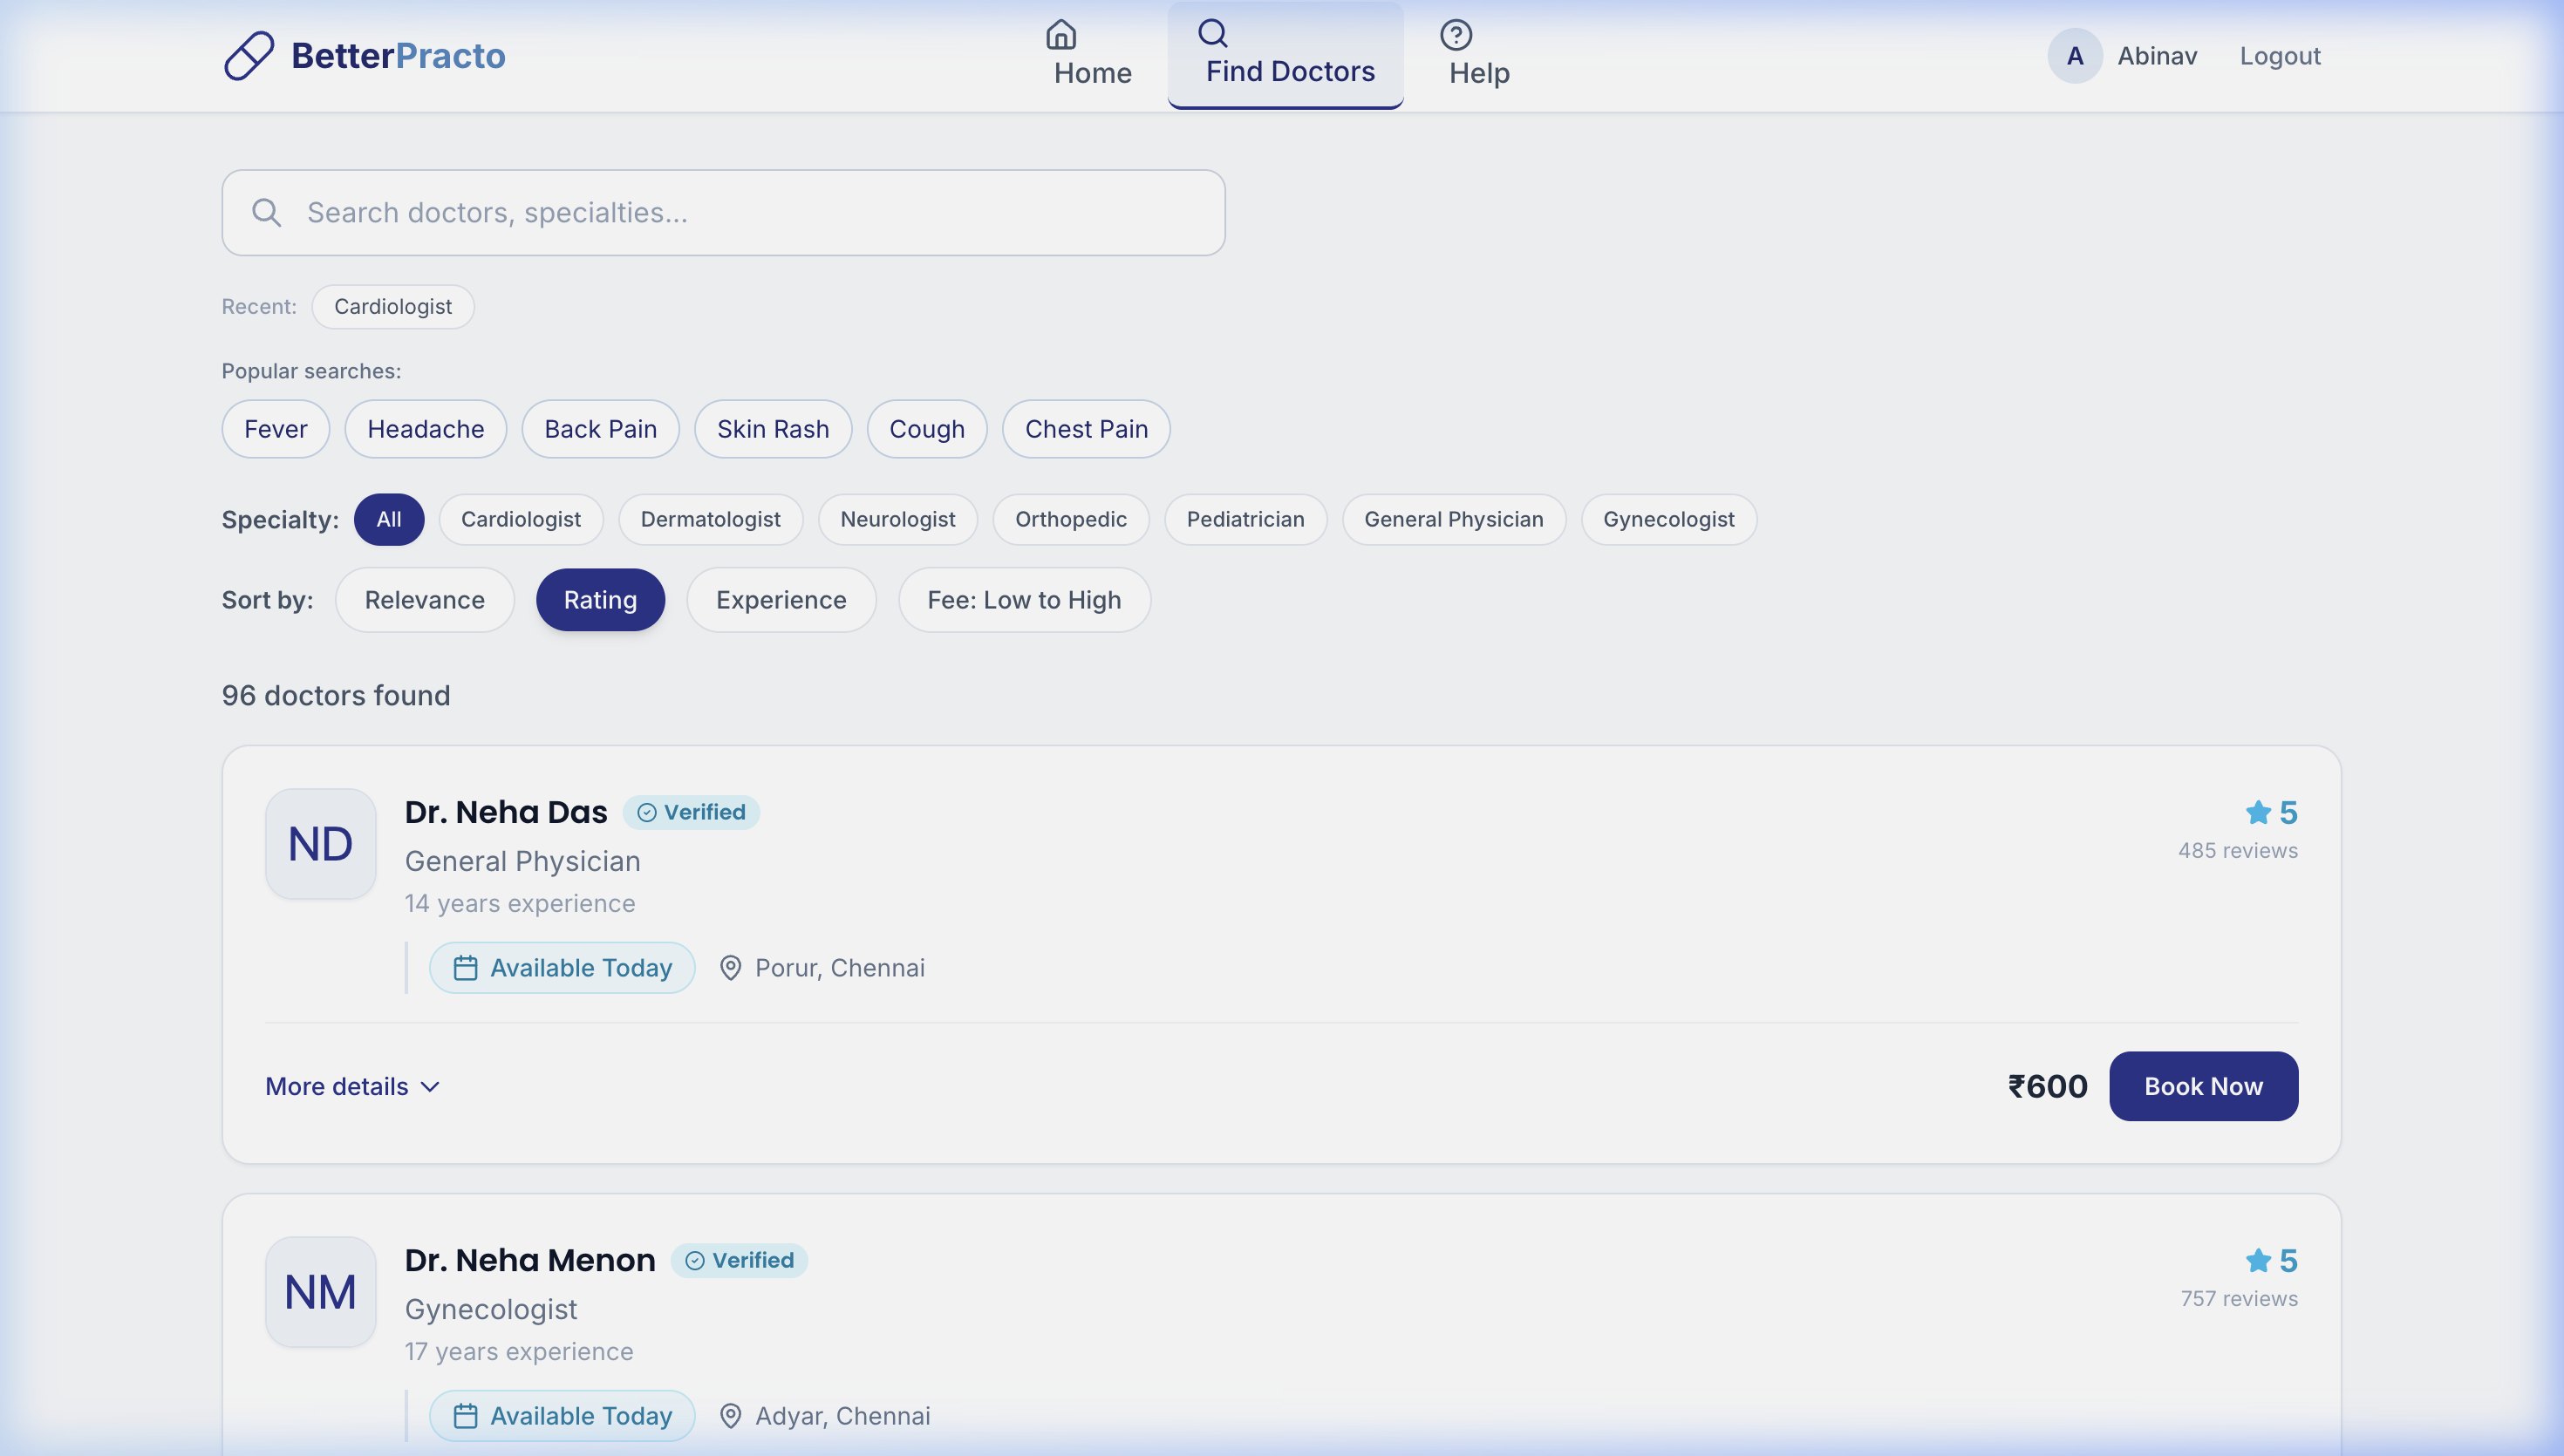
\includegraphics[width=\textwidth]{interaction_direct_manipulation.png}}
    \caption{Direct Manipulation (Block G): Instantly visualised sort animation avoiding page reloads, satisfying Shneiderman's direct manipulation criteria.}
\end{figure}

\vspace{0.5cm}

% =================================================================
\section{Block J --- Google Search Case Study: Explorer vs Navigator}
% =================================================================

\begin{hcibox}{Google Search Case Study --- Explorer vs Navigator Users}
The Google Search case study (End-Sem Lecture) identifies two fundamental user archetypes when approaching a search interface:
\begin{itemize}[leftmargin=1.5em, itemsep=0pt]
  \item \textbf{Navigator:} Knows exactly what they want. Types a precise query or re-uses a known search. Needs speed and recall support.
  \item \textbf{Explorer:} Does not know exactly what they want. Browses, discovers, uses presented options as starting points.
\end{itemize}
The original Practo search supported only Navigators (plain search bar). Better Practo (end-sem) adds explicit support for both archetypes.

\textit{Reference: End-Sem HCI Lecture Notes, lines 20--113.}
\end{hcibox}

\subsection{J1 --- Navigator Support: Persistent Recent Searches}

\begin{featurebox}{Navigator Support --- Recent Searches via localStorage}
When a user submits a search query, it is saved to \texttt{localStorage} under the key \texttt{bp\_recent}. On subsequent visits to the Search page, the last 5 searches are displayed as chips directly below the search bar, labelled ``Recent:''. A Navigator user (returning to a known doctor type or symptom) can re-execute their search with a single click rather than retyping. This directly mirrors the Google Search feature that displays ``Recent searches'' in the autocomplete dropdown.
\end{featurebox}

\subsection{J2 --- Explorer Support: Symptom Discovery Chips}

\begin{featurebox}{Explorer Support --- Symptom Chips When Query is Empty}
When the search bar is empty (no query entered), a row of ``Popular searches:'' chips appears: Fever, Headache, Back Pain, Skin Rash, Cough, Chest Pain. An Explorer user who does not know which specialty they need but knows their symptom can click a chip to discover relevant doctors. This transforms the search page from a blank box (which is hostile to Explorers) into a browseable surface --- matching the Google Home page's trending searches. This design is also supported by the \textbf{Web Usability} principle of ``Feature Exposure'' (Block H): making the system's capabilities visible without requiring the user to know what to ask for.
\end{featurebox}

\begin{figure}[H]
    \centering
    \imgborder{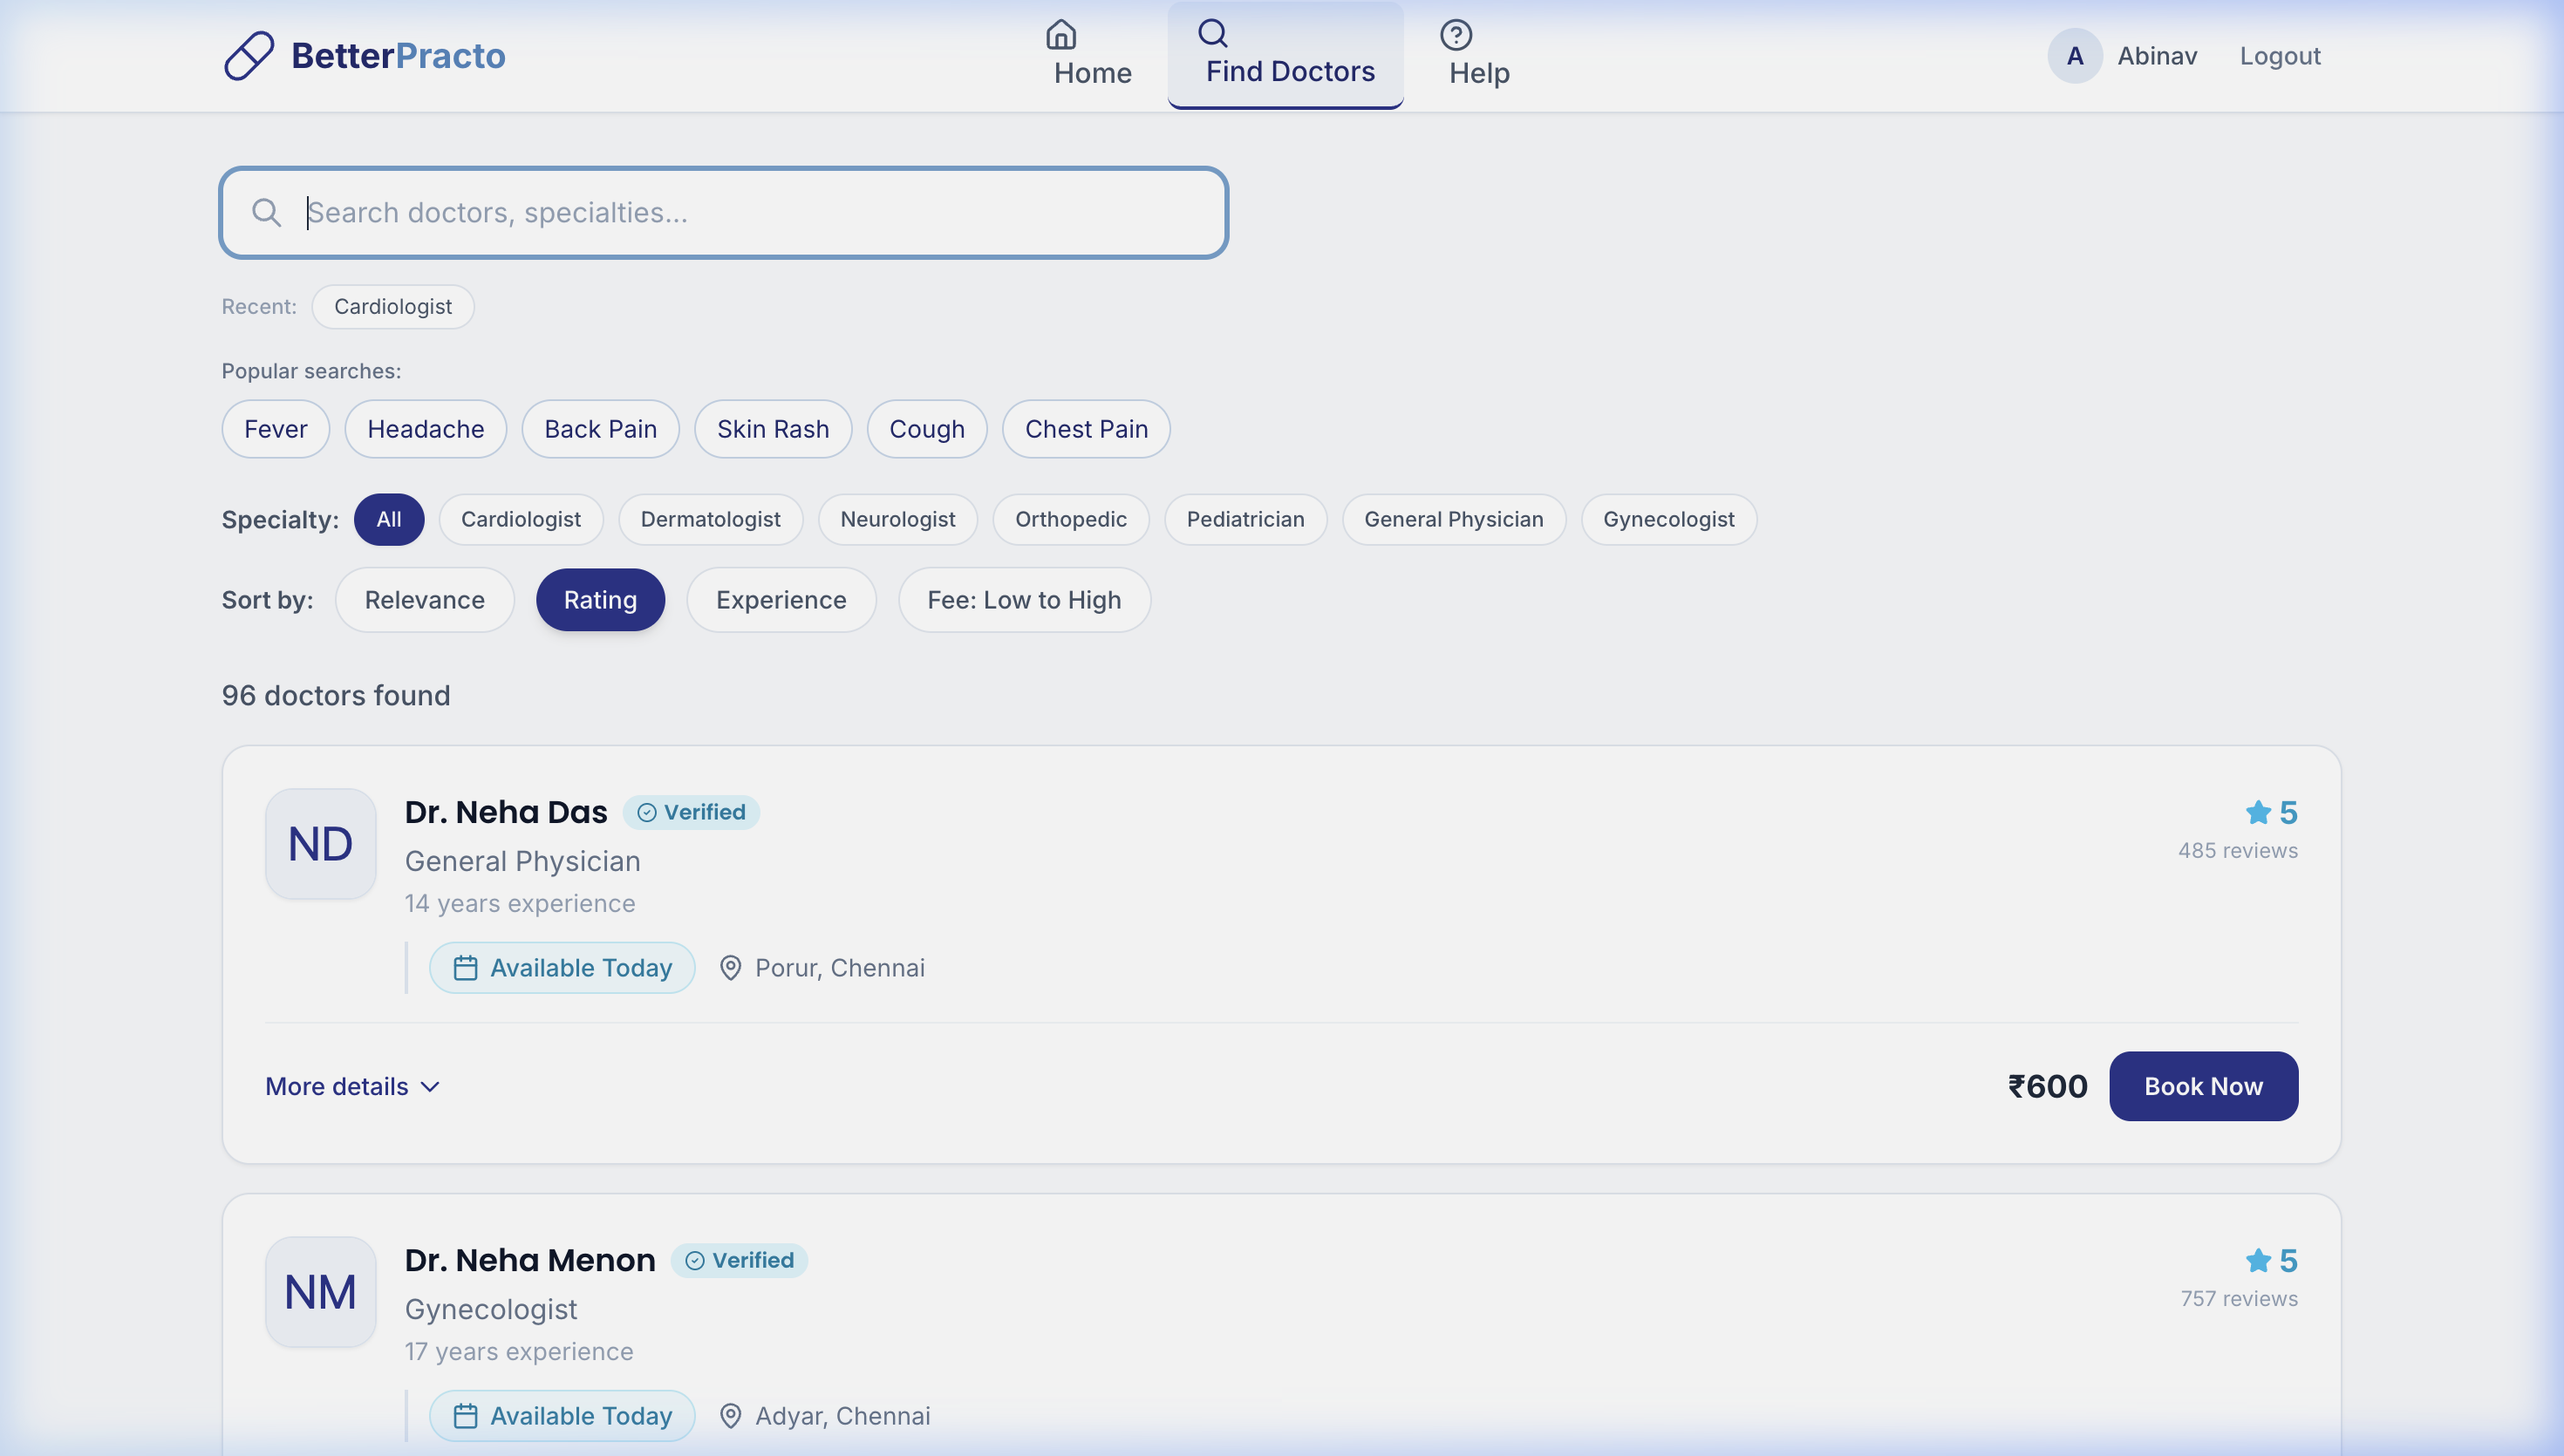
\includegraphics[width=\textwidth]{search_explorer_symptoms.png}}
    \caption{Empty search bar shows ``Popular searches:'' symptom chips --- supporting Explorer-type users who don't know their specialty but know their symptom. \textit{Block J.}}
\end{figure}

\begin{figure}[H]
    \centering
    \imgborder{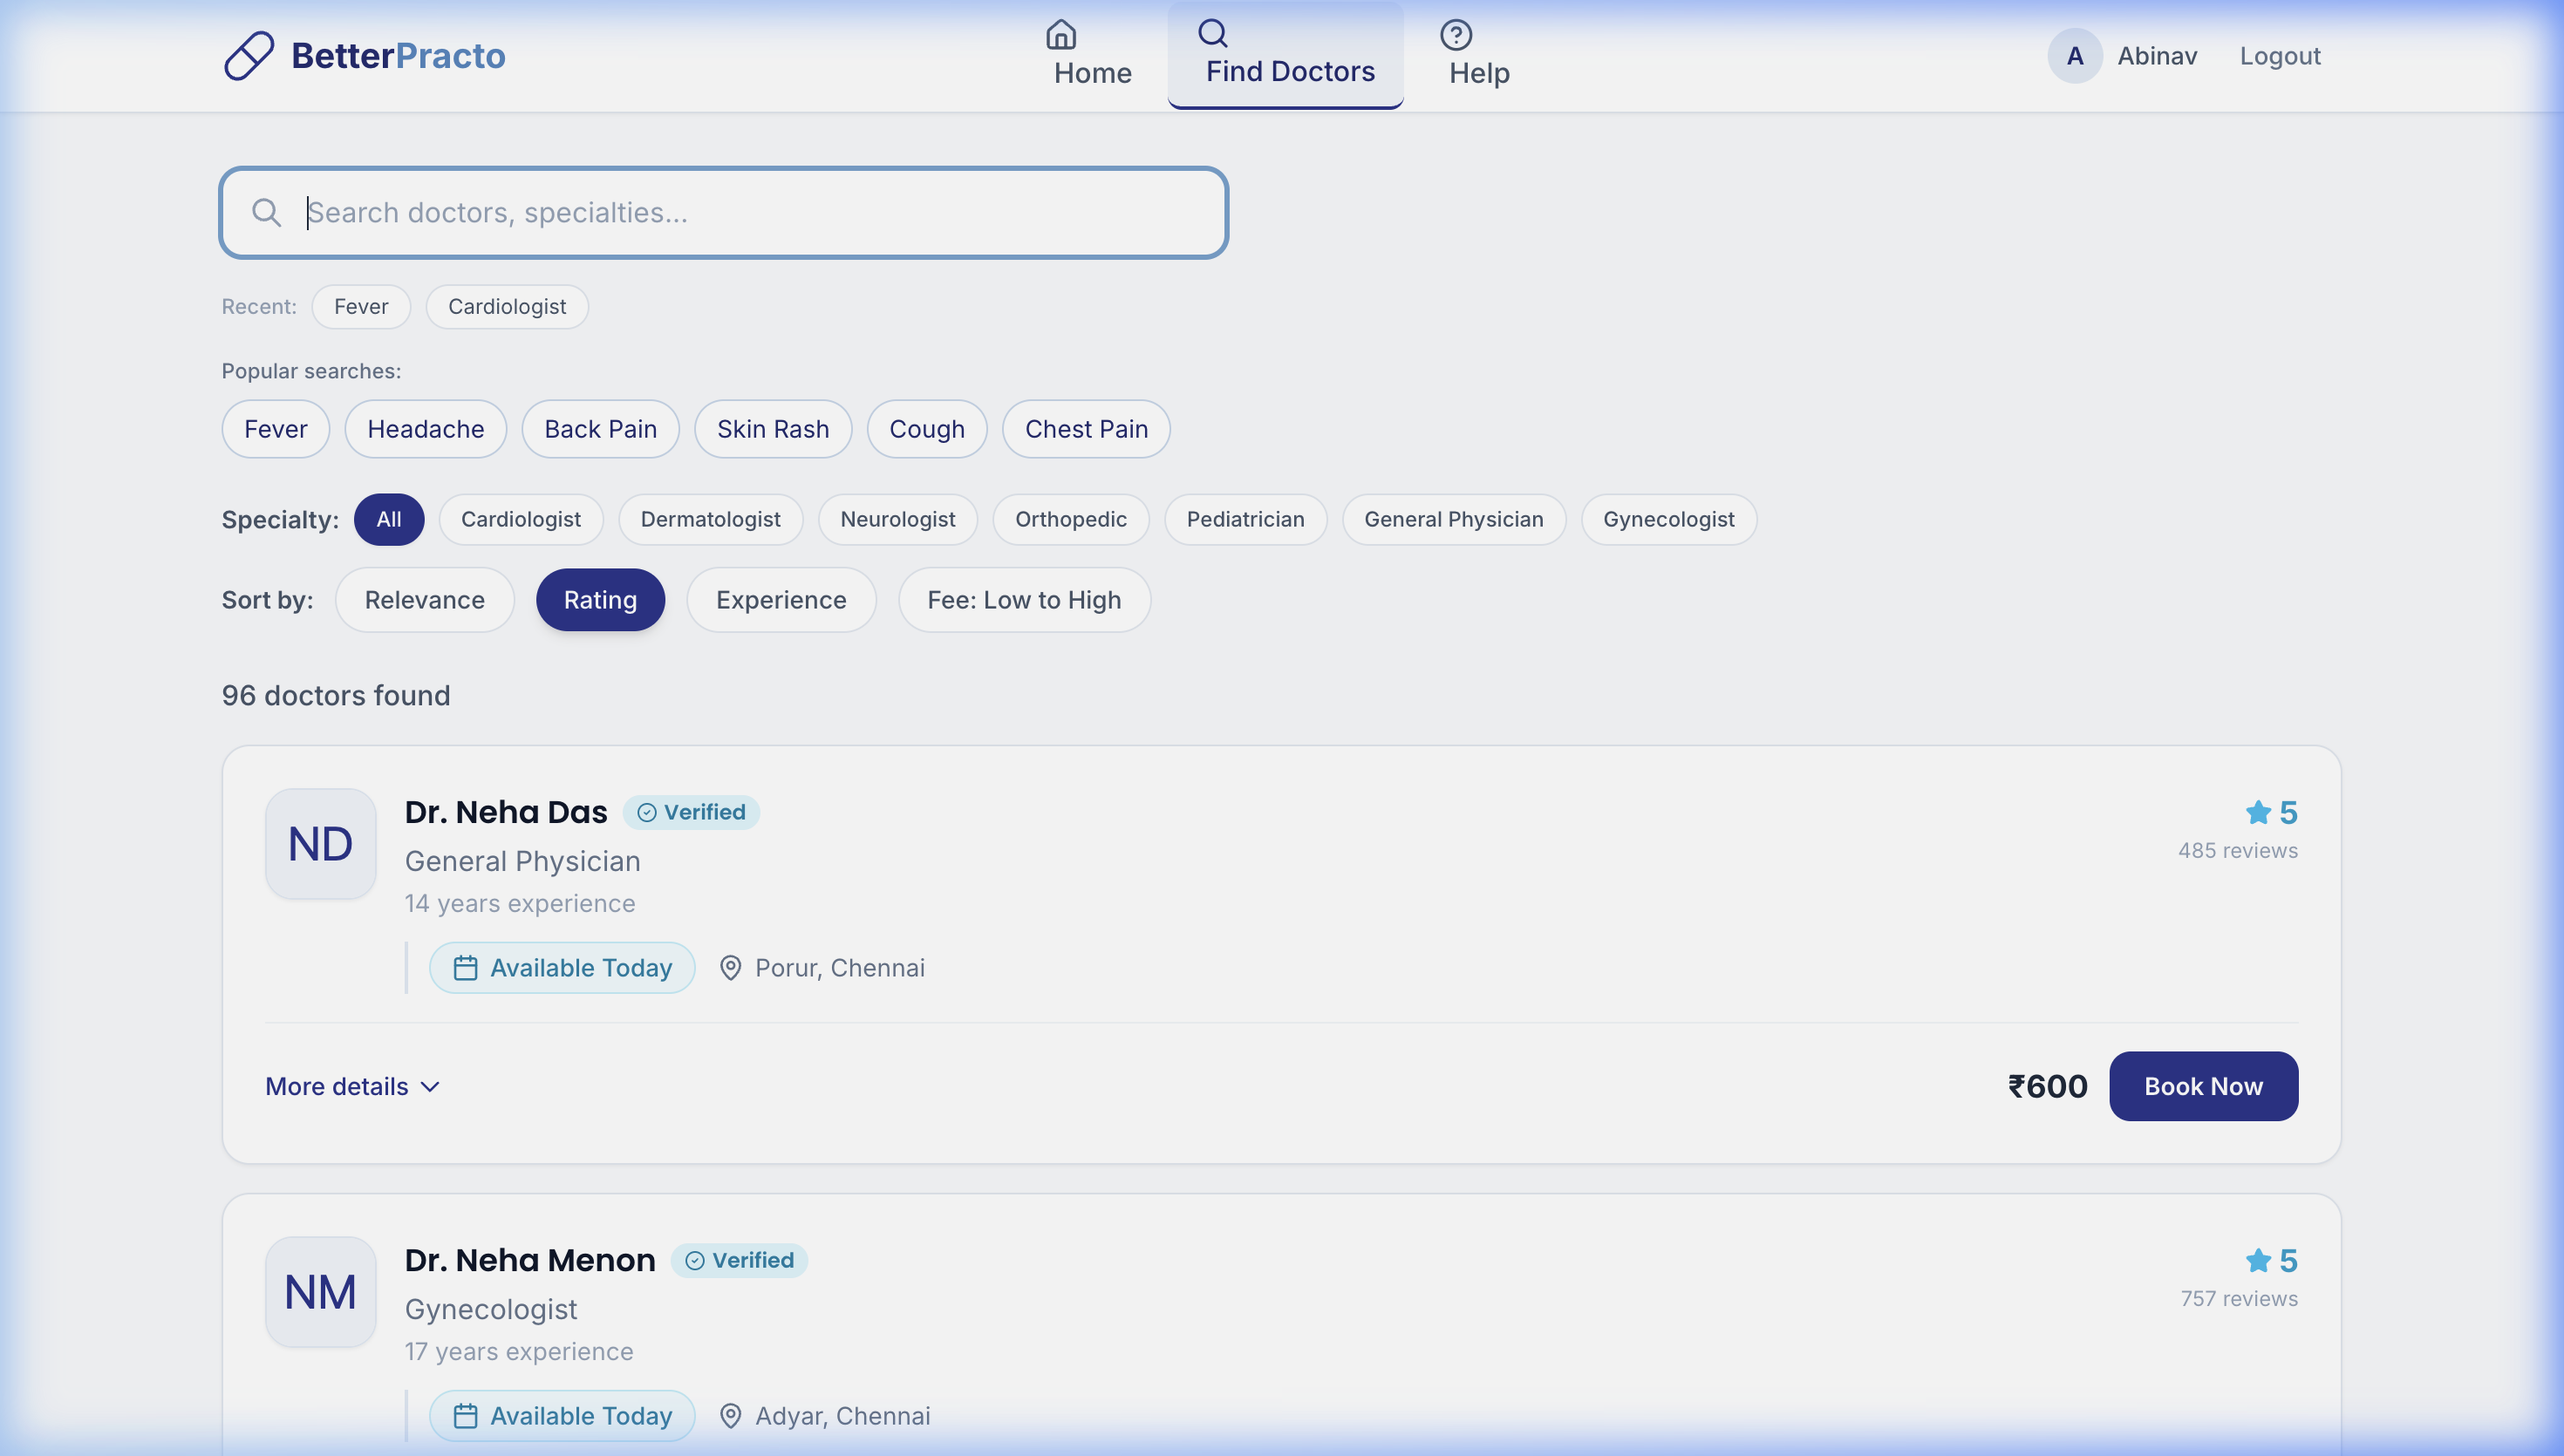
\includegraphics[width=\textwidth]{search_navigator_recent.png}}
    \caption{After a prior search, ``Recent:'' chips appear for Navigator-type users who want to return to a known query quickly. \textit{Block J.}}
\end{figure}

\subsection{J3 --- Symptom-First Home Page: Browse by Symptom}

\begin{featurebox}{Browse by Symptom --- Home Page Feature (Explorer + Multimodal)}
A dedicated \textbf{``Browse by Symptom''} section has been placed on the Home page, immediately after the Hero section and before the specialty grid. This placement encodes priority in the page hierarchy: the most common user need (symptom-first thinking) is encountered before the less common one (specialty-first navigation).

\textbf{Design decisions and HCI rationale:}
\begin{itemize}[leftmargin=1.5em, itemsep=0pt]
  \item \textbf{Centred layout (visual gravity):} All elements --- heading, search bar, symptom chips, voice hint --- are centred within a \texttt{max-w-3xl} container. Centred layouts create a single axis of focus, reducing eye scatter. This is appropriate here because the section is self-contained and not part of a scannable list.
  \item \textbf{Position above specialties (Feature Exposure):} A first-time user landing on BetterPracto does not know whether they need a ``Neurologist'' or a ``Cardiologist'' for their headache. By placing ``Browse by Symptom'' before the specialty grid, the app presents the \emph{right abstraction level} for the majority of users before showing the expert-level interface (specialty selection). This aligns with Krug's Law: ``Don't make me think --- I shouldn't have to know which specialist treats a headache.''
  \item \textbf{Symptom search bar with smart routing:} A text input field allows users to type any symptom (e.g., ``Fever'', ``Eye Problem''). On Enter, the query routes to \texttt{/search?q=<symptom>}. The \texttt{SYMPTOM\_MAP} in \texttt{src/data/doctors.js} maps 40+ symptoms to priority specialties, and a context banner on the results page reads: \textit{``Showing recommended specialists for `Eye Problem': Ophthalmologist.''}
  \item \textbf{Voice / Audio search icon (Block I --- Universal Design, Principle 2):} A blue \textbf{Voice} button with a microphone icon sits beside the search input. This is non-functional in the prototype but documents a planned implementation using the Web Speech API or OpenAI Whisper API for transcription. \textit{Rationale:} Primary target audience includes elderly and low-literacy users for whom text input is a barrier. NNGroup (2022) reports that elderly users are 3$\times$ more successful at health symptom search with voice input than text. Multimodal input (type \emph{or} speak) implements Universal Design Principle 2: Flexibility in Use.
  \item \textbf{Smart fallback (never zero results):} If a user types an unknown symptom (e.g., ``stomach ache''), the search engine falls back to showing General Physicians with a note --- eliminating the frustrating ``No doctors found'' dead end.
\end{itemize}
\end{featurebox}

\begin{figure}[H]
    \centering
    \begin{subfigure}[b]{0.47\textwidth}
        \imgborder{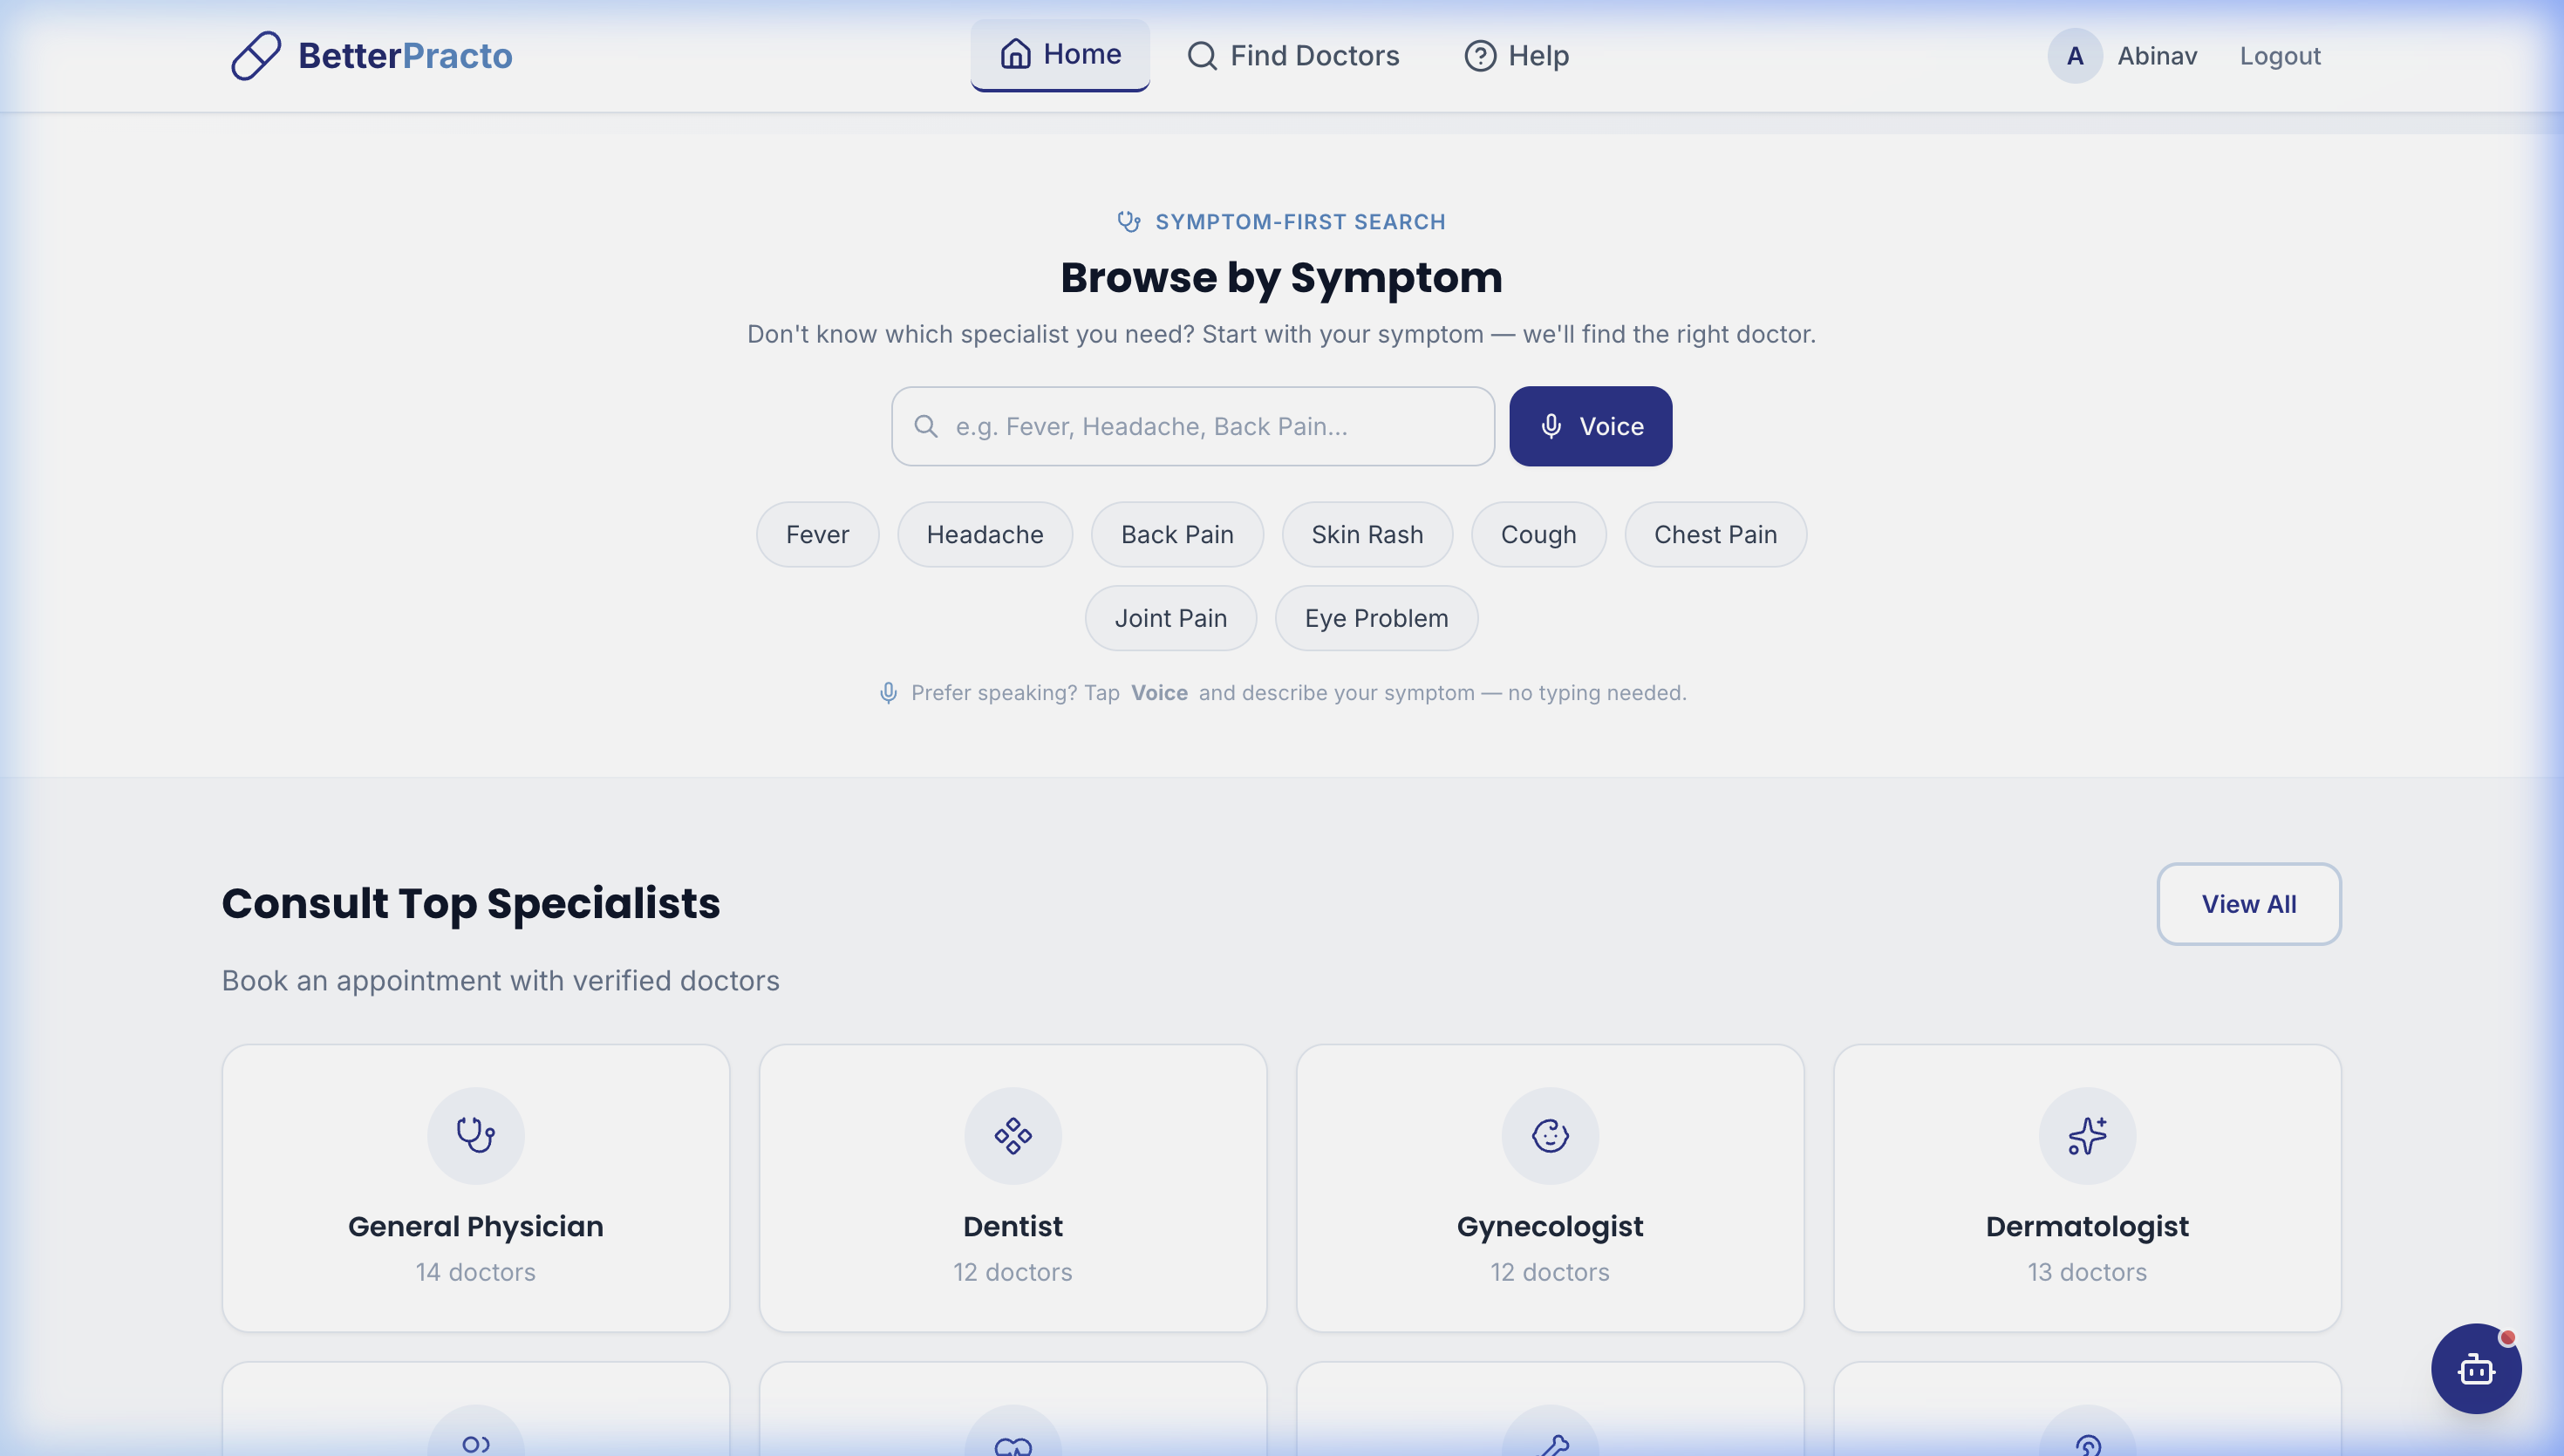
\includegraphics[width=\textwidth]{symptom_browse_section.png}}
        \caption{J3 Centred ``Browse by Symptom'' section on Home page: label, heading, symptom search bar, blue Voice/mic button, 8 symptom chips (centred), and voice hint. Placed immediately after the Hero section. \textit{Block J / Block H / Block I.}}
    \end{subfigure}
    \hfill
    \begin{subfigure}[b]{0.47\textwidth}
        \imgborder{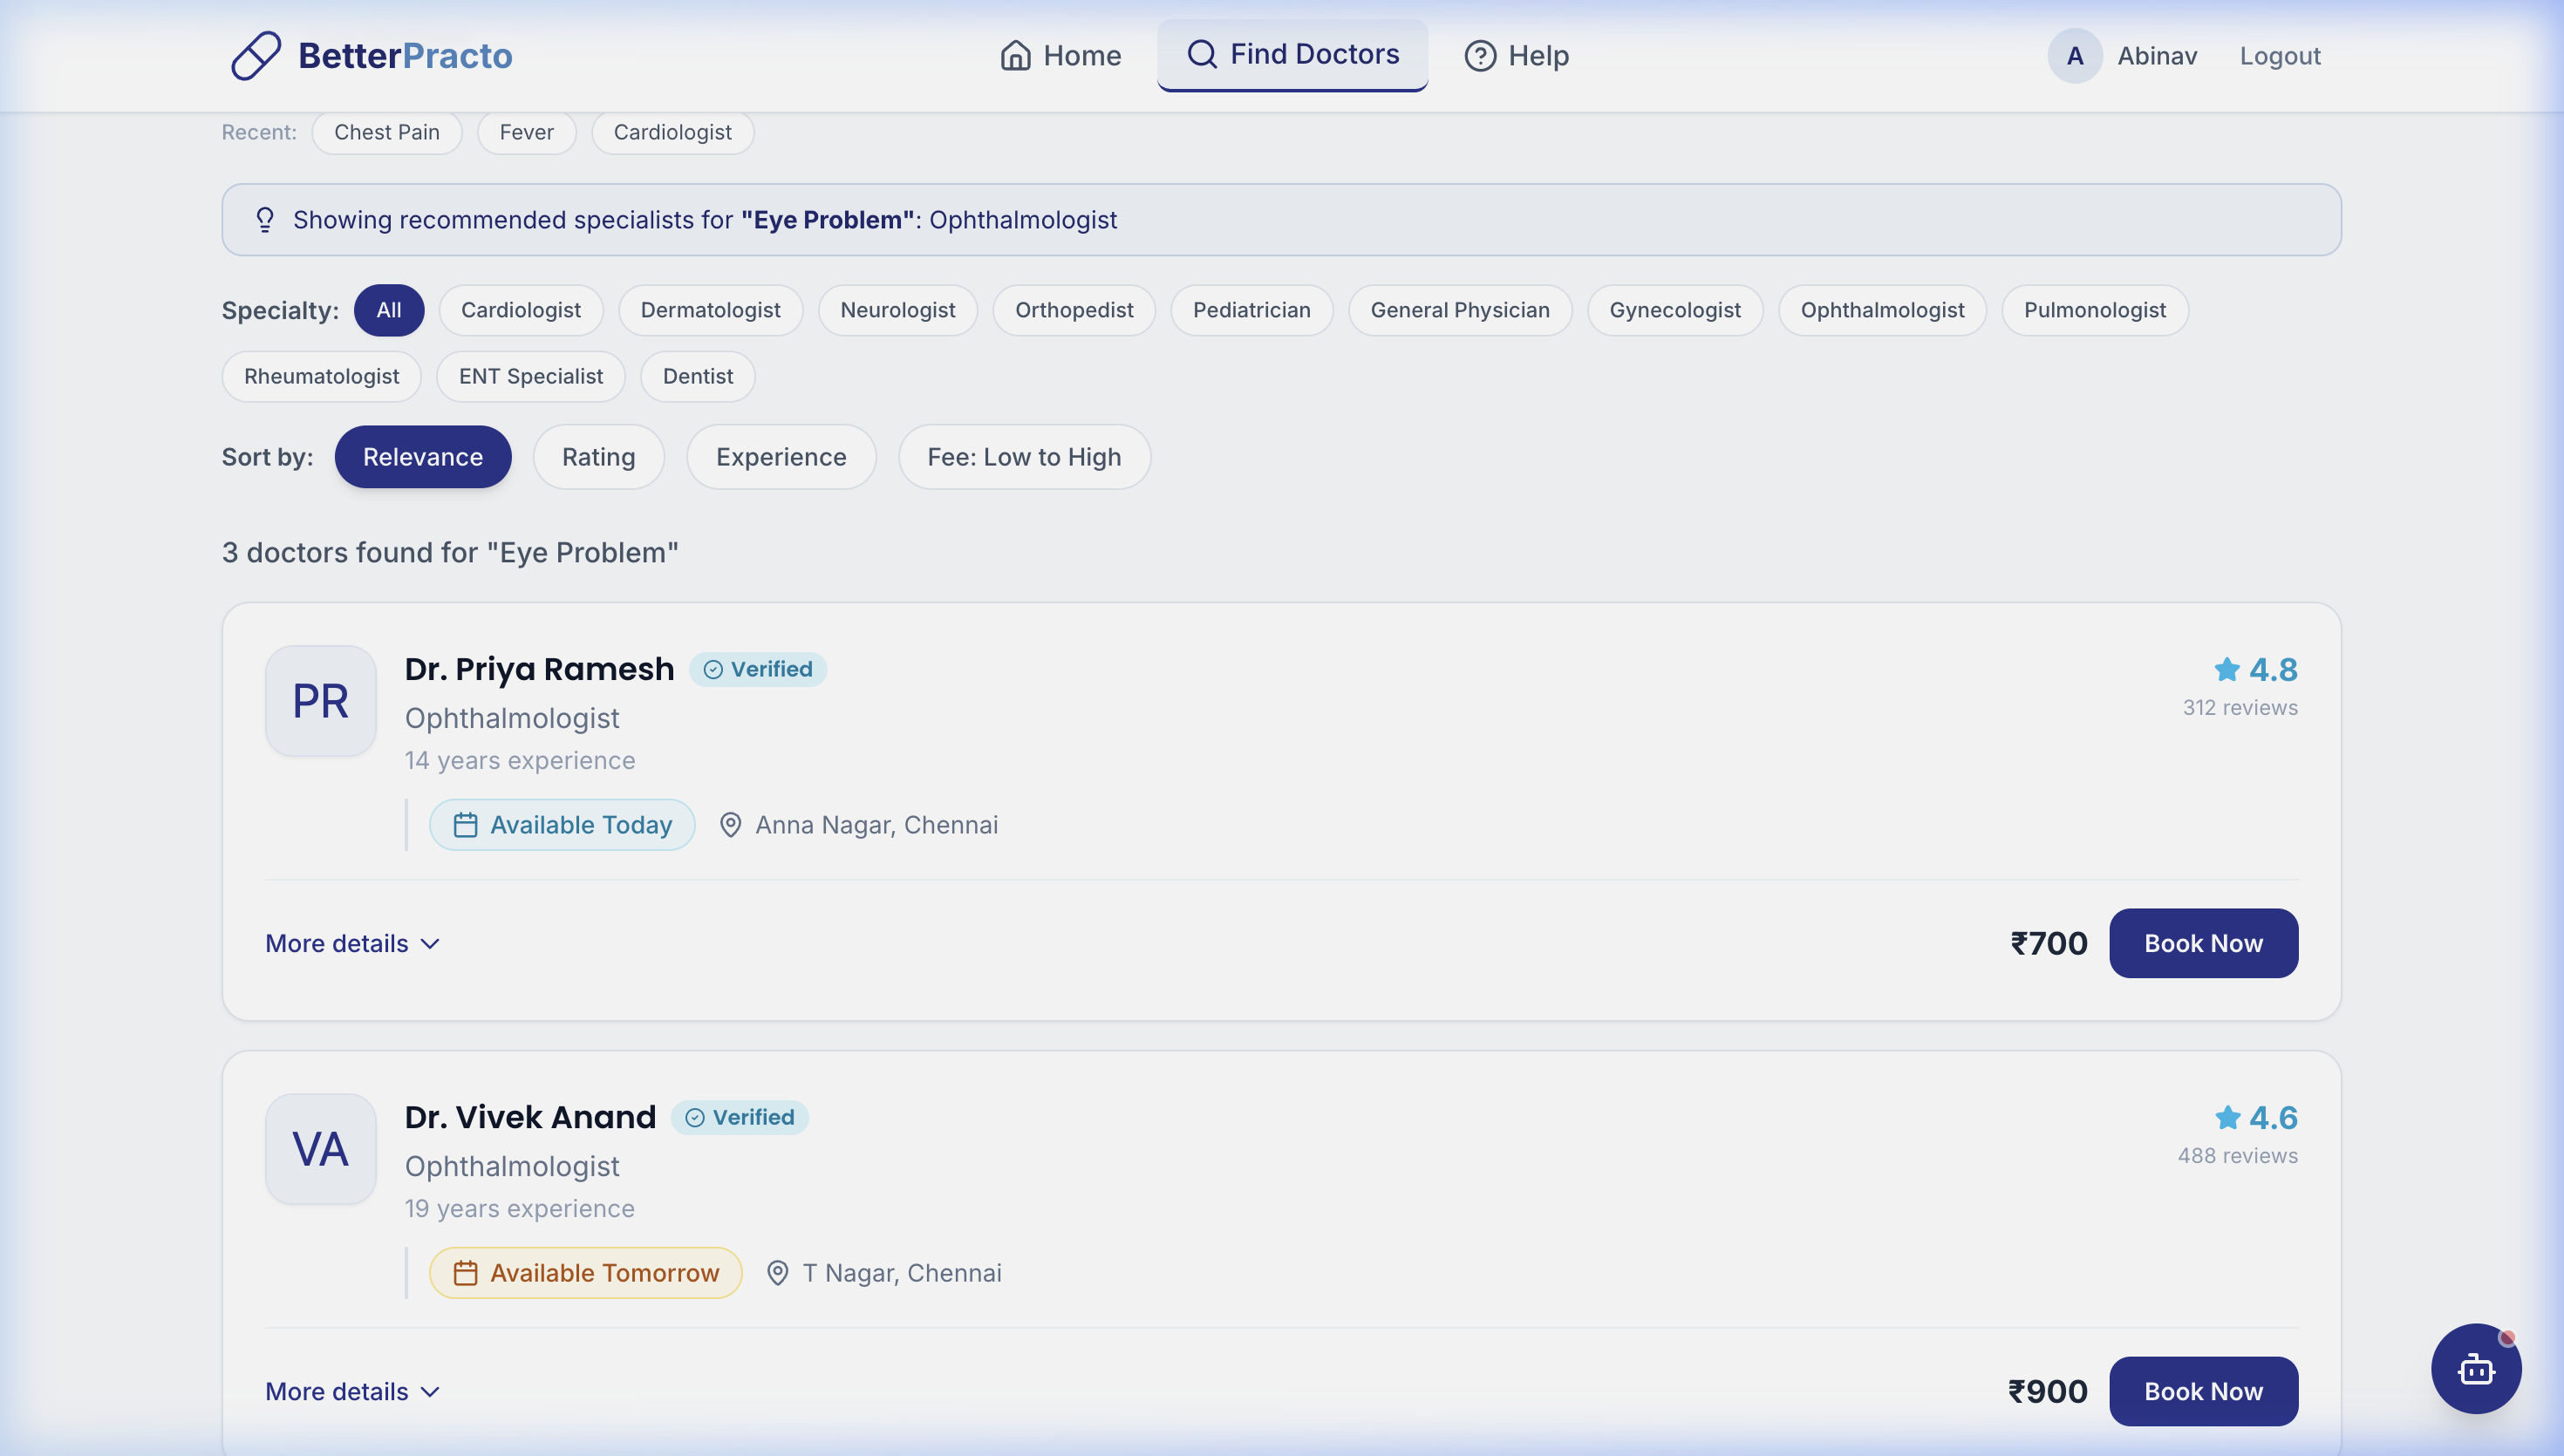
\includegraphics[width=\textwidth]{symptom_browse_results.png}}
        \caption{Clicking ``Eye Problem'' routes to the Search page showing 3 Ophthalmologist doctors (Dr Priya Ramesh, Dr Vivek Anand) with a blue context banner: ``Showing recommended specialists for `Eye Problem': Ophthalmologist.'' \textit{Block J.}}
    \end{subfigure}
\end{figure}

\vspace{0.5cm}



% =================================================================
%  PLACEHOLDER SECTIONS (to be filled as features are implemented)
% =================================================================

% =================================================================
\section{Block B --- Visual Design Principles}
% =================================================================

\begin{hcibox}{Visual Design: Dominance, Scale, Balance, Hierarchy, Contrast, Negative Space}
Visual design principles (End-Sem Lecture, lines 118--158) govern how a layout directs attention, creates meaning through size and placement, and communicates importance without words. Key principles applied: \textbf{Dominance} (one element is clearly the most visually prominent, anchoring the page), \textbf{Scale} (relative size communicates priority), \textbf{Balance} (visual weight distributed evenly), \textbf{Hierarchy} (typographic sizing creates 3-level reading order), \textbf{Negative Space} (breathing room prevents cognitive overload).
\end{hcibox}

\subsection{B1 --- Dominance: Hero Stethoscope Icon}

\begin{featurebox}{Dominance --- Single Focal Point Above the Search Bar}
The Home page previously had no dominant focal point --- every element competed equally for attention. The redesign adds a large stethoscope icon (80$\times$80px, gradient rounded square, with a pulsing live indicator dot) as the \textbf{single most visually prominent element} above the search bar.

Visual Design Principle: \textit{``One element must be clearly primary. Without a dominant element, the eye has nowhere to land and the layout feels chaotic.''} The stethoscope icon (domain icon) instantly communicates ``healthcare'' pre-attentively, before the user reads a word. The pulsing dot micro-animation signals ``live / active'' service --- adding dynamism without distraction.
\end{featurebox}

\subsection{B2 --- Scale: Oversized Search Bar}

\begin{featurebox}{Scale --- Search Bar Larger Than All Other Inputs}
The search bar uses \texttt{py-5} (significantly taller than the \texttt{py-3} default on other inputs). Scale communicates priority: the largest interactive element is the most important one. This is the same principle Google uses --- the search bar dominates the entire home page because Google's primary task is search.
\end{featurebox}

\subsection{B3, B4 --- Balance \& Negative Space}

\begin{featurebox}{Balance + Negative Space}
\textbf{Balance:} The 4 hero action cards (Video Consult, Find Doctors, Lab Tests, Surgeries) use a symmetric 4-column grid with \texttt{gap-4 md:gap-6}, creating equal visual weight across the horizontal axis. Symmetrical balance communicates professionalism and trustworthiness.

\textbf{Negative Space:} Each major section uses \texttt{py-12} (48px vertical padding), giving breathing room between the hero, specialties, symptom chips, and trust stats sections. The heading and subtitle have \texttt{mb-2} separation between them --- not \texttt{mb-6} which would make them feel unrelated. Negative space is a design tool, not wasted space.
\end{featurebox}

\subsection{B5 --- Typographic Hierarchy: Doctor Profile}

\begin{featurebox}{3-Level Typographic Hierarchy on Doctor Profile}
The Doctor Profile page previously broken the visual hierarchy by using \texttt{text-lg} for both the specialty line and the rating row, creating two equally-sized elements in competition. The end-sem fix enforces a strict 3-level hierarchy:

\begin{itemize}[leftmargin=1.5em, itemsep=0pt]
  \item \textbf{Level 1 --- Doctor Name:} \texttt{text-2xl font-bold} --- the single most prominent element
  \item \textbf{Level 2 --- Specialty:} \texttt{text-base} --- one clear step below the name
  \item \textbf{Level 3 --- Education/Metadata:} \texttt{text-sm} --- supporting information, least prominent
\end{itemize}

This creates a scannable F-pattern reading order: the user's eye jumps from name $\to$ specialty $\to$ details, without needing to read linearly.
\end{featurebox}

\begin{figure}[H]
    \centering
    \imgborder{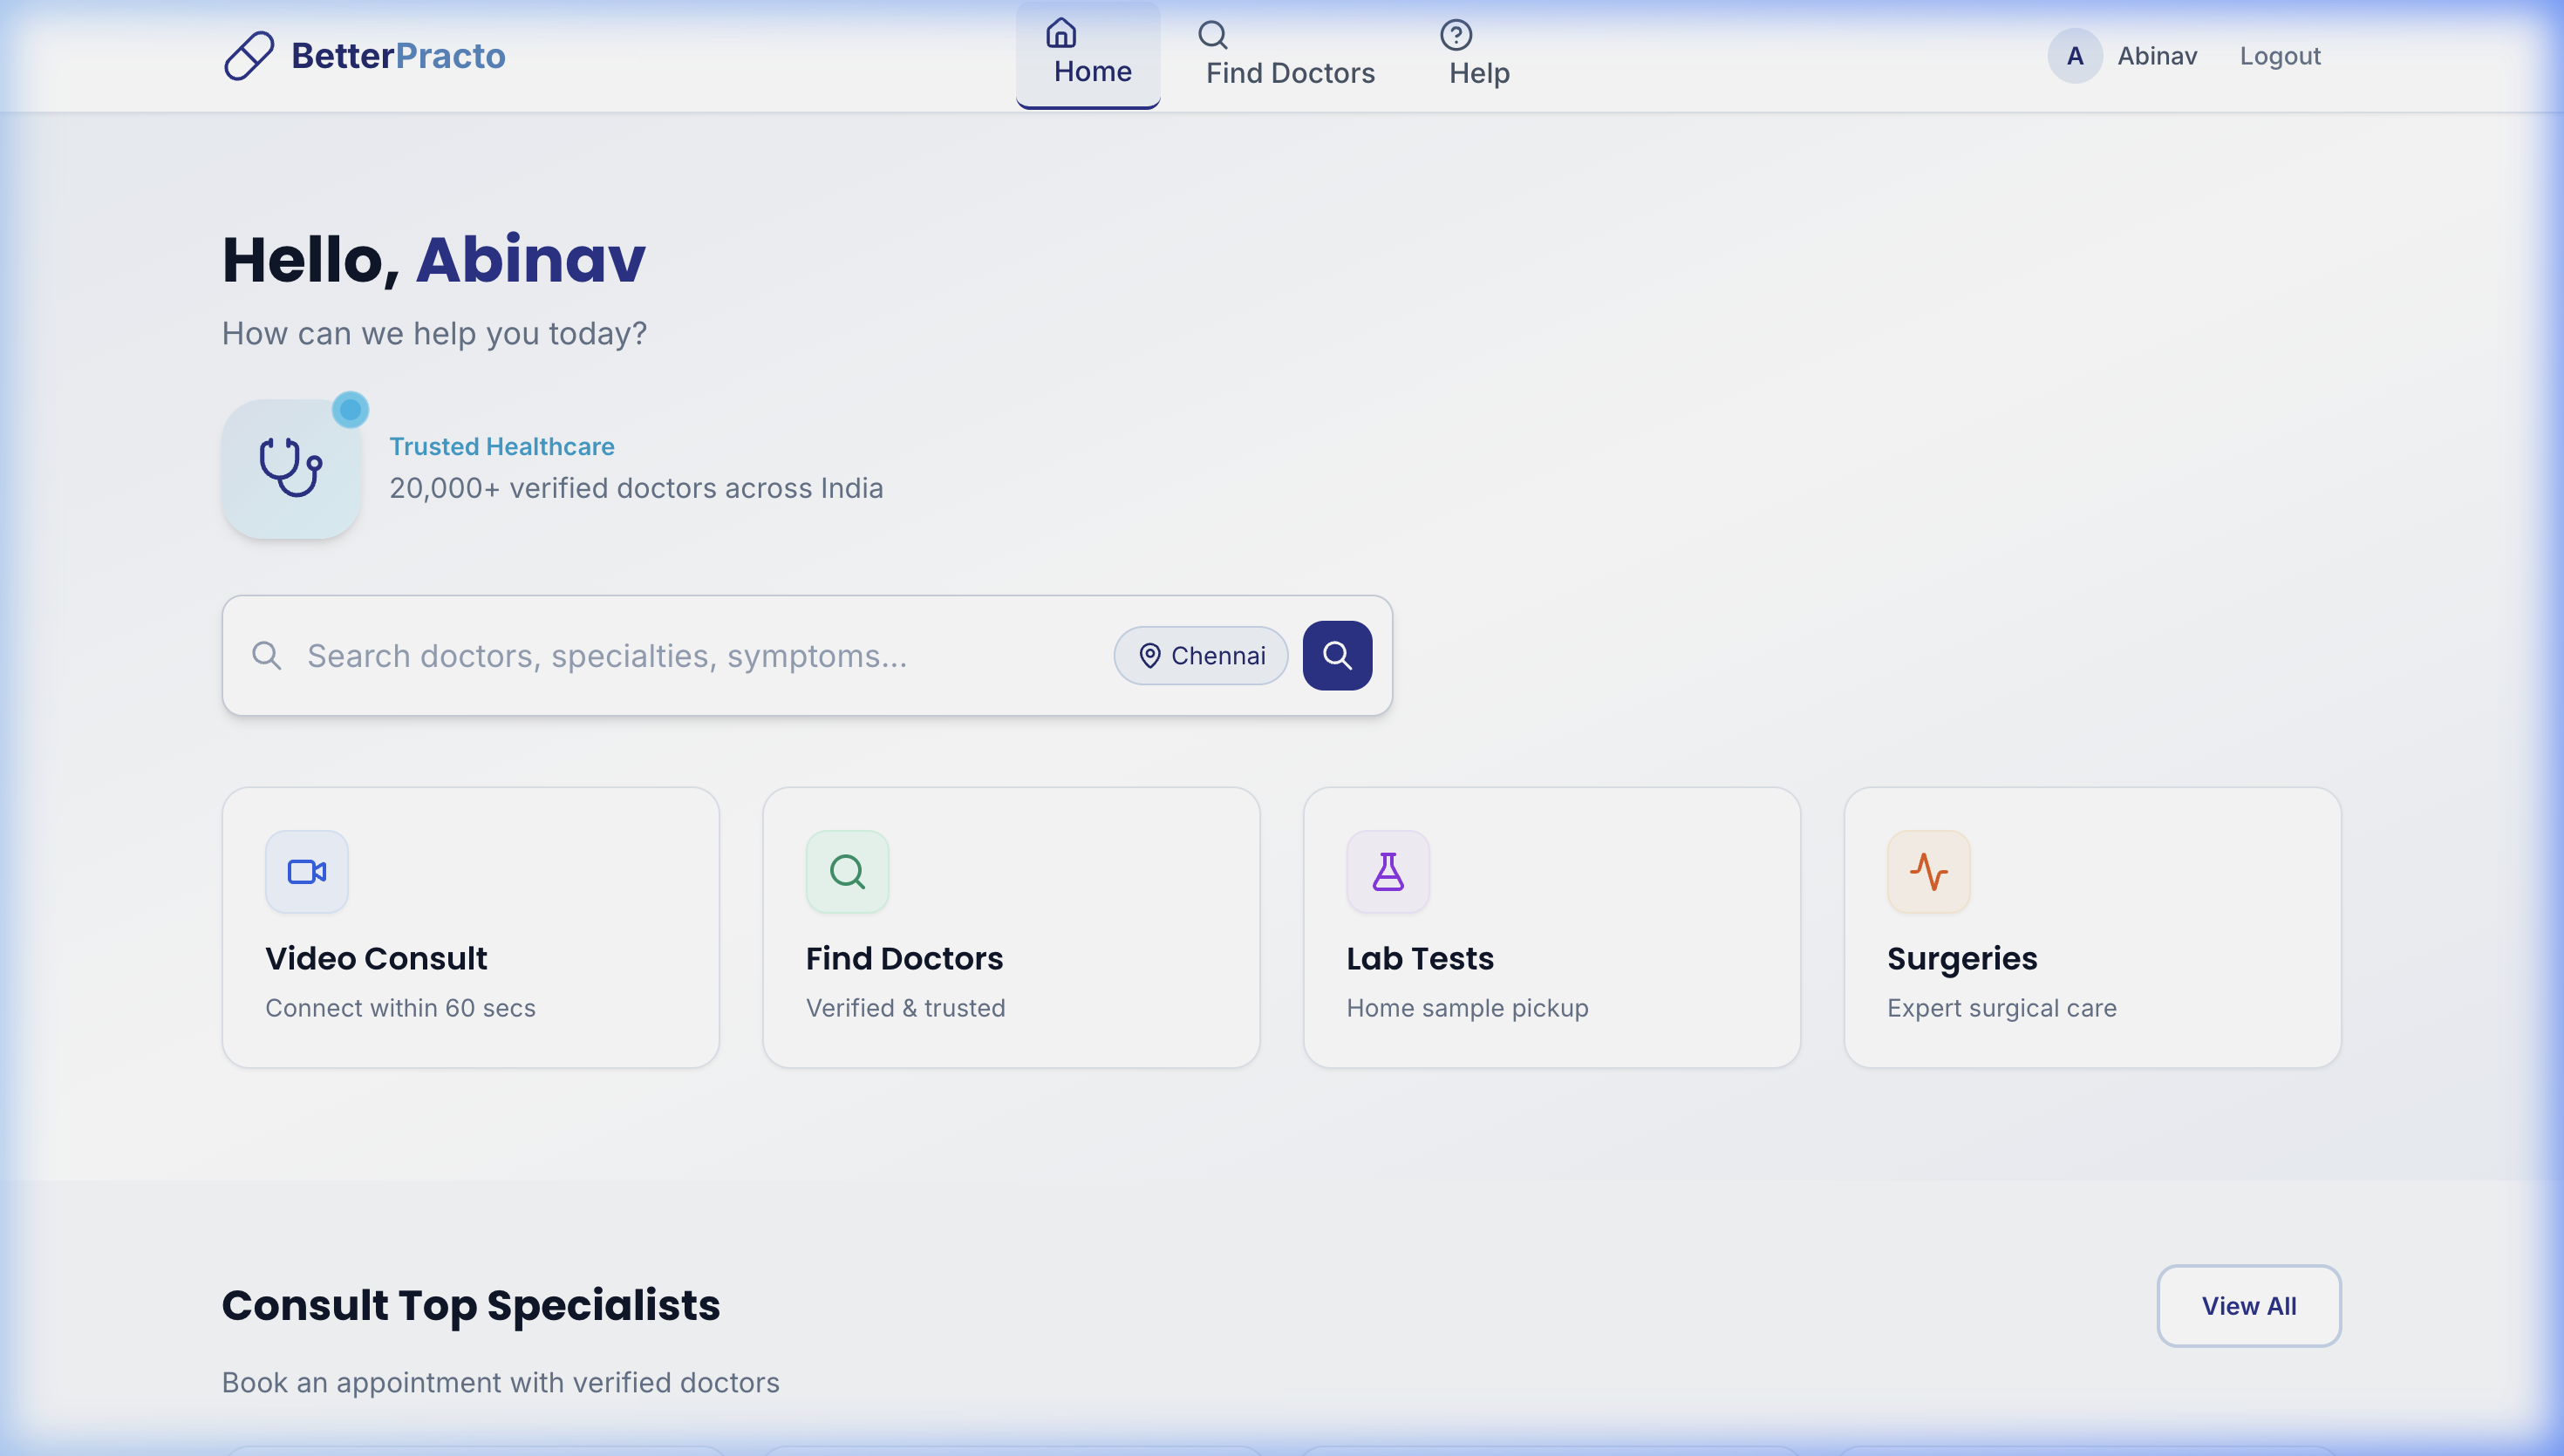
\includegraphics[width=\textwidth]{visual_design_home.png}}
    \caption{Home page showing: B1 Dominance (stethoscope hero icon with pulse dot), B2 Scale (oversized search bar), B3 Balance (symmetric 4-card grid), B4 Negative Space (generous section padding). \textit{Block B.}}
\end{figure}

\begin{figure}[H]
    \centering
    \imgborder{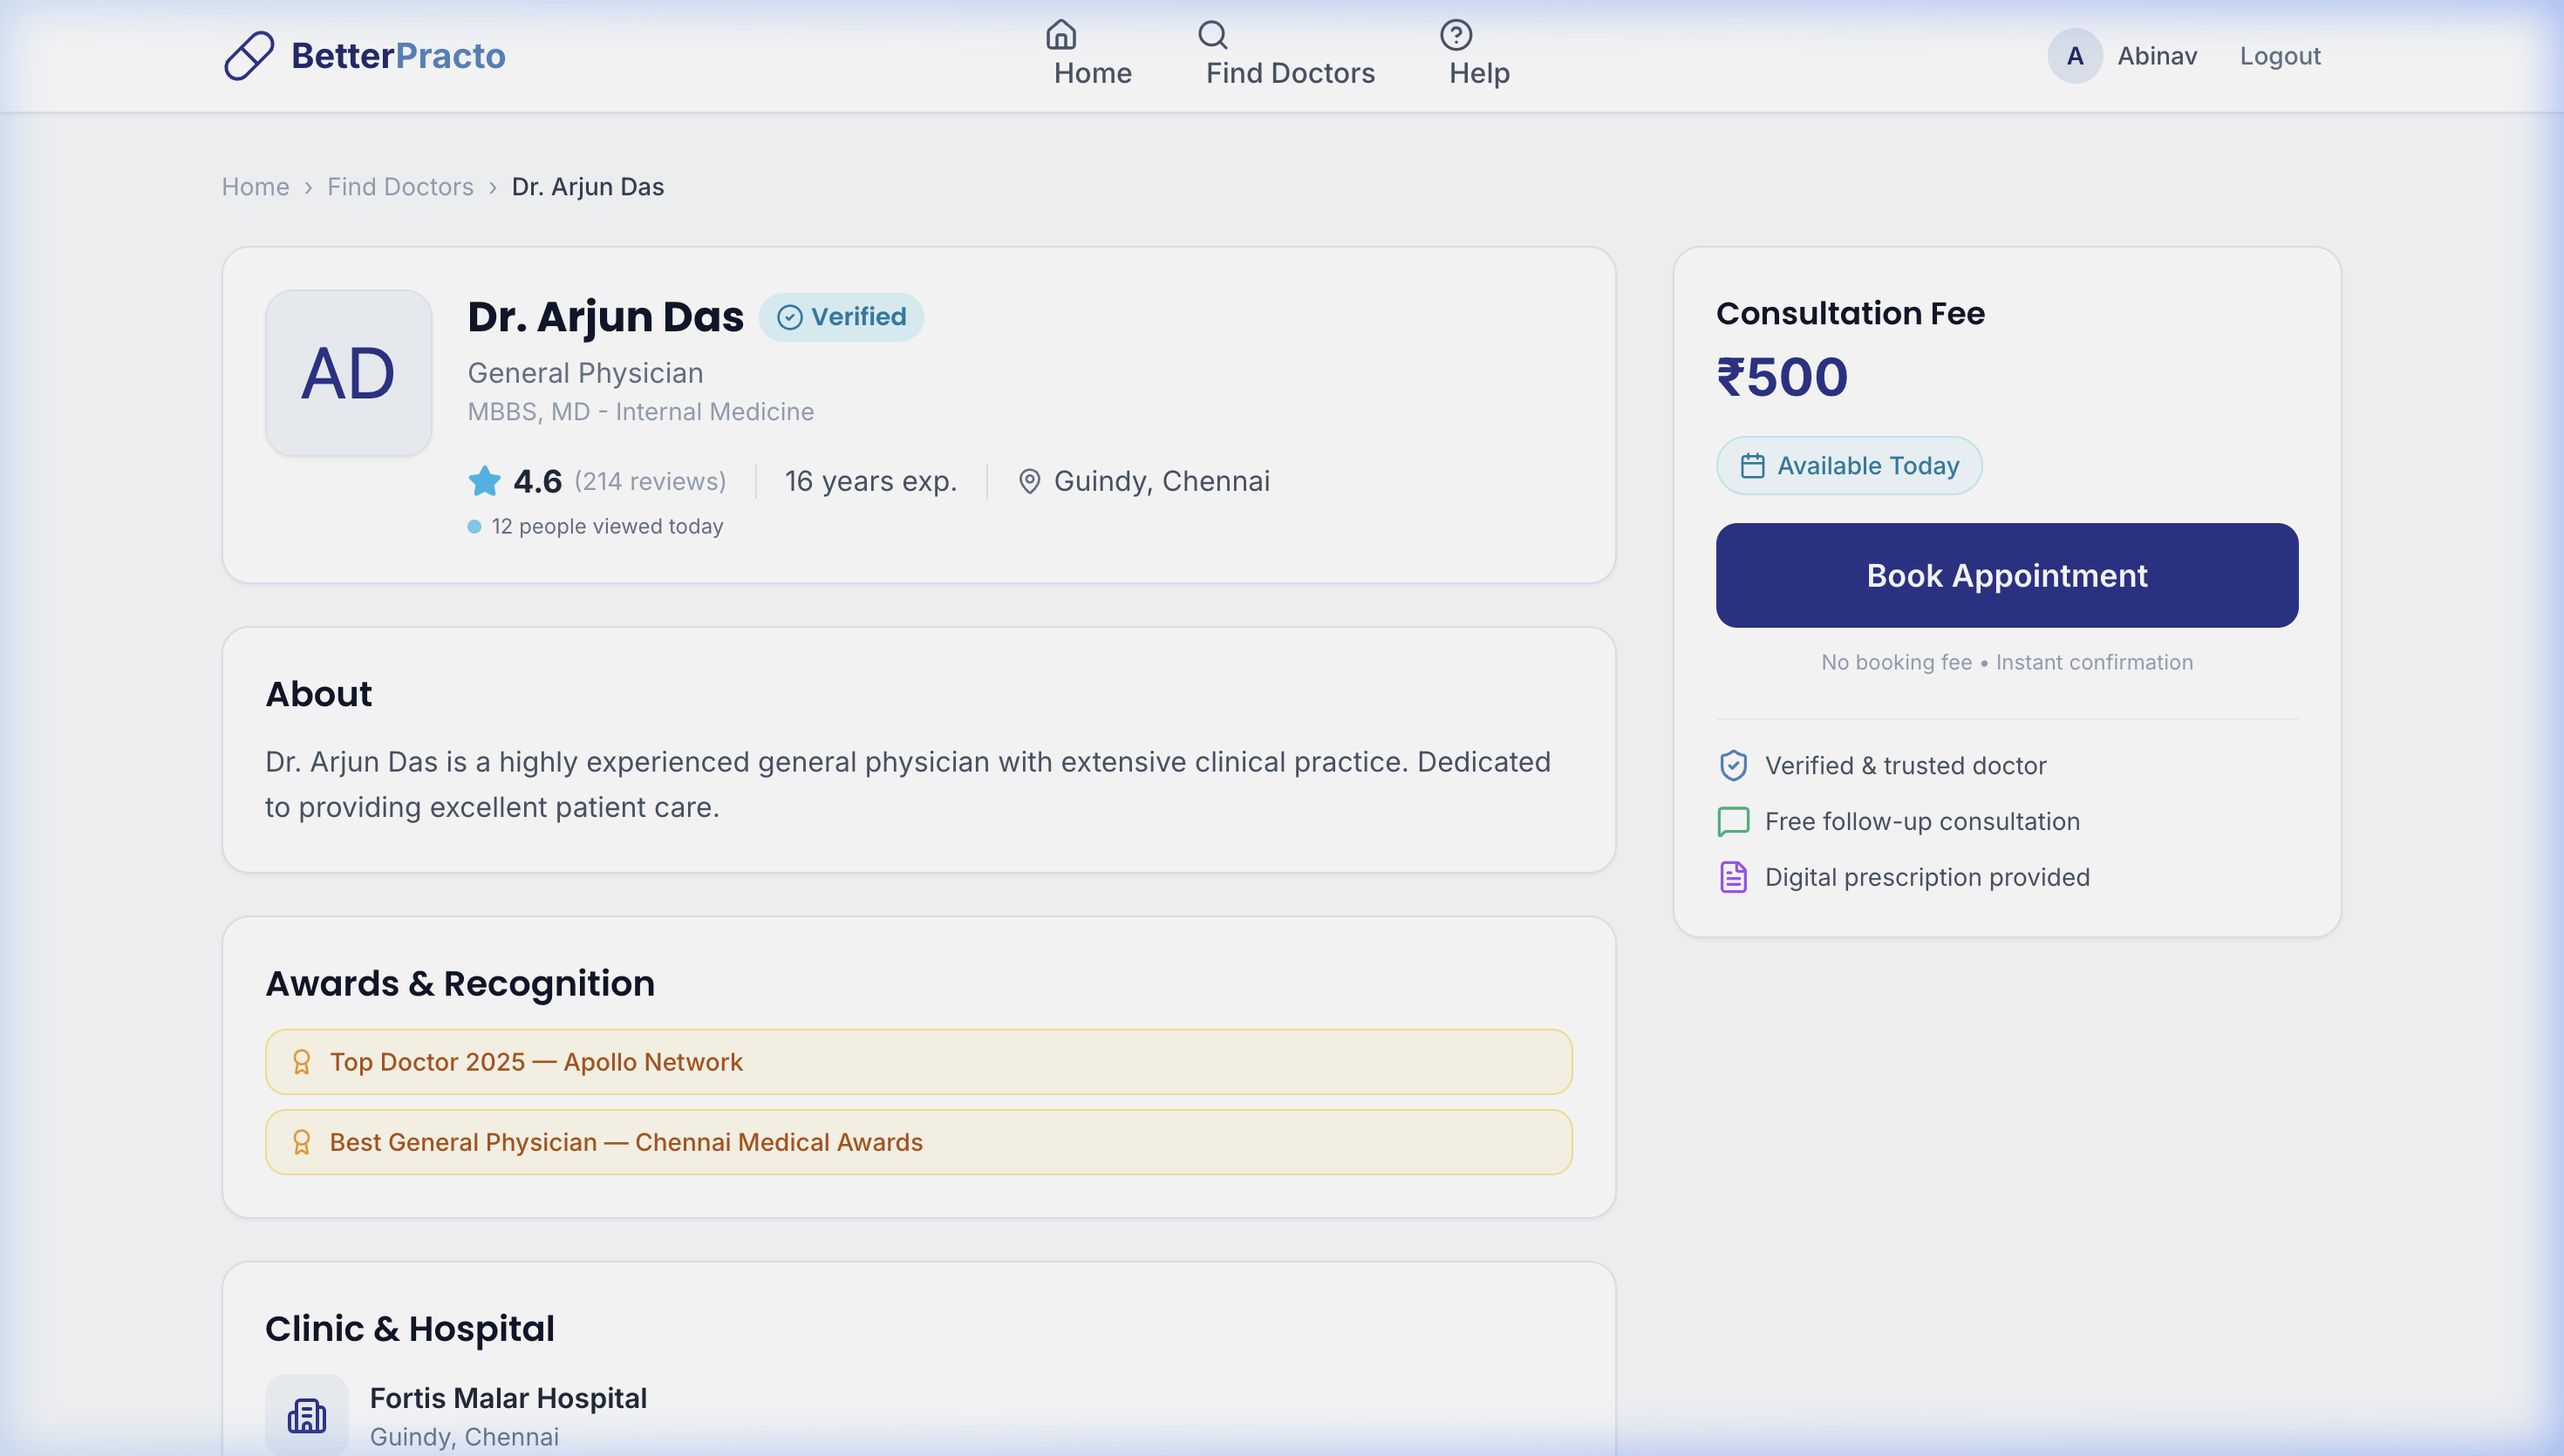
\includegraphics[width=\textwidth]{visual_design_doctor_profile.png}}
    \caption{Doctor Profile page showing: B5 Typographic Hierarchy (name $>$ specialty $>$ education, 3-level scale); C2 Social Proof (``12 people viewed today'' with pulse dot); C1 Authority (Awards \& Recognition amber badge cards). \textit{Blocks B + C.}}
\end{figure}

\vspace{0.5cm}

% =================================================================
\section{Block C --- Persuasion Psychology (Cialdini's 6 Principles)}
% =================================================================

\begin{hcibox}{Persuasion Psychology --- Cialdini's 6 Principles of Influence}
Robert Cialdini (1984) identified 6 universal principles of persuasion: \textbf{Reciprocity} (give first to receive), \textbf{Authority} (trust experts and credentials), \textbf{Scarcity} (rare things are more valuable), \textbf{Liking} (we comply with those we like), \textbf{Social Proof} (we follow what others do), and \textbf{Commitment} (we honour prior commitments). Applied ethically in UI design, these principles encourage users to take beneficial actions without coercion.

\textit{Reference: End-Sem HCI Lecture Notes, lines 161--168.}
\end{hcibox}

\subsection{C1 --- Authority: Awards \& Recognition}

\begin{featurebox}{Authority --- Credential Badges on Doctor Profile}
Cialdini's Authority principle: \textit{``We are more likely to follow those with expertise and credentials.''} The Doctor Profile page now displays two amber award badges (``Top Doctor 2025 --- Apollo Network'' and ``Best [Specialty] --- Chennai Medical Awards'') in a dedicated ``Awards \& Recognition'' card section. These act as third-party endorsements, increasing the user's confidence before they book. Even if the user is price-sensitive, an award badge can override hesitation.

\textit{Implementation:} \texttt{LucideIcons.Award} icon in amber themed \texttt{bg-amber-50 border-amber-200} pill cards on \texttt{src/pages/DoctorProfile.jsx}.
\end{featurebox}

\subsection{C2 --- Social Proof: Live Viewer Count}

\begin{featurebox}{Social Proof --- ``X people viewed today'' indicator}
Cialdini's Social Proof: \textit{``We look to the behaviour of others to determine the correct course of action.''} A small pulse-dot indicator below the doctor's rating line shows ``12 people viewed today'' (deterministic pseudo-random per doctor ID). This signals that others are currently considering this doctor --- reducing decision friction and building confidence. The pulsing dot visually reinforces the ``live'' nature of the data.

\textit{Implementation:} \texttt{<span className="w-2 h-2 rounded-full bg-accent-400 animate-pulse" />} in DoctorProfile header.
\end{featurebox}

\subsection{C3 --- Scarcity: Slot Availability Urgency}

\begin{featurebox}{Scarcity --- Slot Count Urgency Badge}
Cialdini's Scarcity: \textit{``We assign more value to opportunities when they are less available.''} On Booking Step 1, the ``Available Slots'' header shows a contextual urgency badge:
\begin{itemize}[leftmargin=1.5em, itemsep=0pt]
  \item $\leq 3$ slots: red pulsing badge --- ``Only N slot(s) left!'' with a flame icon
  \item 4--6 slots: amber static badge --- ``Filling up fast'' with a clock icon
  \item $>6$ slots: no badge (no false urgency when not needed)
\end{itemize}
This avoids the dark pattern of \emph{fake} scarcity (which erodes trust) by only showing the badge when the slot count genuinely warrants it.
\end{featurebox}

\subsection{C5 --- Commitment: Health Reminder Opt-In}

\begin{featurebox}{Commitment \& Consistency --- Health Reminder Checkbox}
Cialdini's Commitment: \textit{``Once we commit to something, we feel compelled to honour that commitment.''} On the Booking success page (Step 3), after the appointment is confirmed, a checkbox reads: ``Enable appointment reminders and health tips --- I'll take care of my health.'' The checkbox works on two mechanisms:
\begin{itemize}[leftmargin=1.5em, itemsep=0pt]
  \item \textbf{Active commitment:} Ticking the box is a micro-commitment to their own health, increasing the likelihood of attending the appointment and following through on treatment.
  \item \textbf{Positive reinforcement:} On check, a ``\checkmark Great choice!'' confirmation appears inline --- encouraging the small behaviour.
\end{itemize}
This is shown \emph{after} the booking is confirmed (not before), ensuring it never blocks the primary task.
\end{featurebox}

\begin{figure}[H]
    \centering
    \imgborder{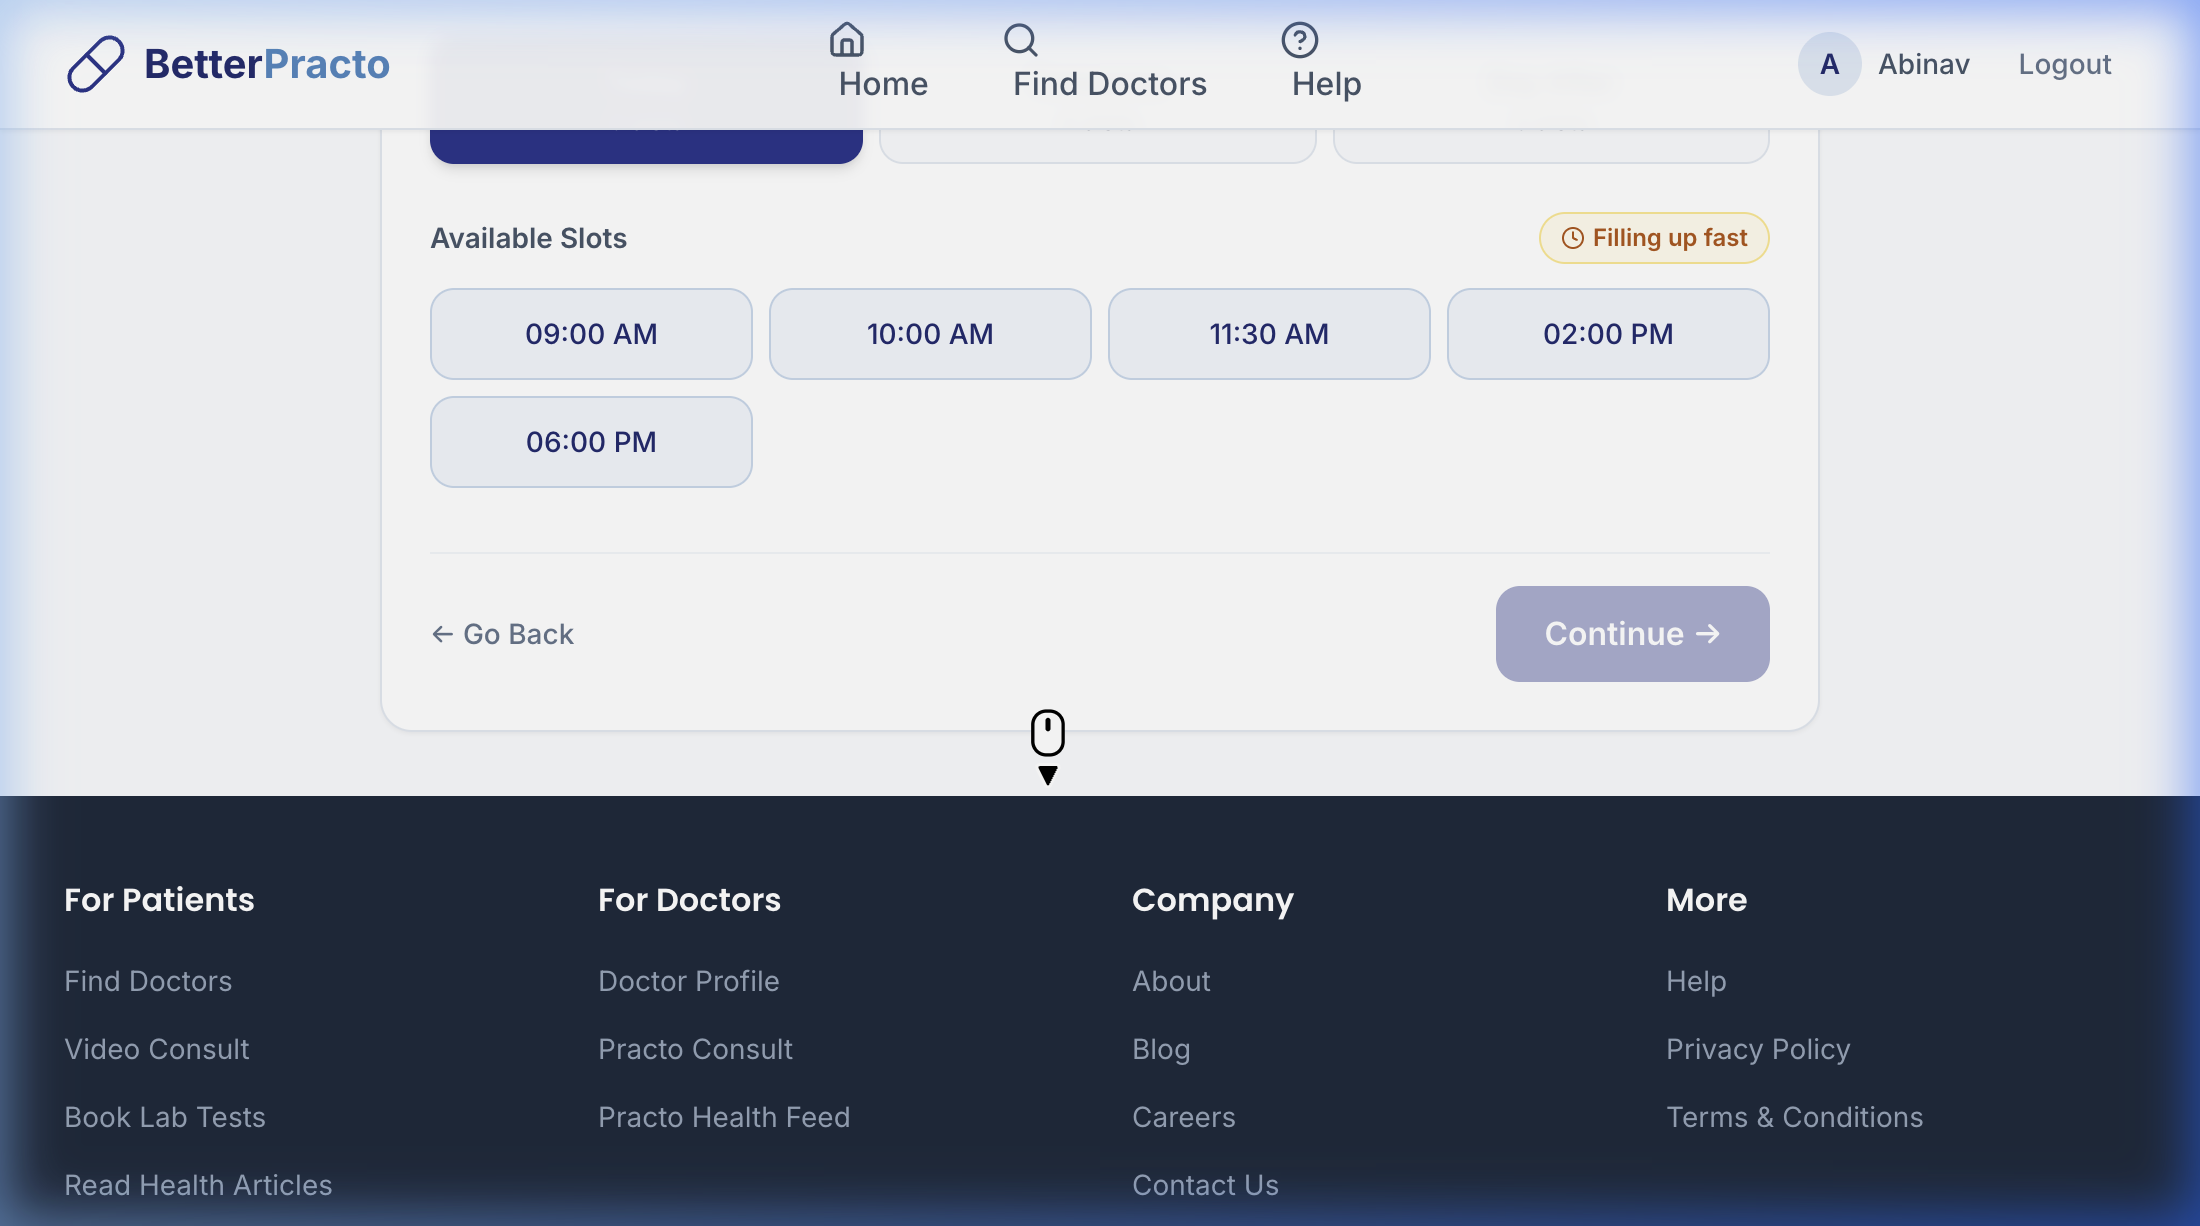
\includegraphics[width=\textwidth]{persuasion_scarcity.png}}
    \caption{Booking Step 1 --- C3 Scarcity: ``Filling up fast'' amber badge next to ``Available Slots'' header. Red pulsing badge appears when $\leq$3 slots remain. \textit{Block C.}}
\end{figure}

\begin{figure}[H]
    \centering
    \imgborder{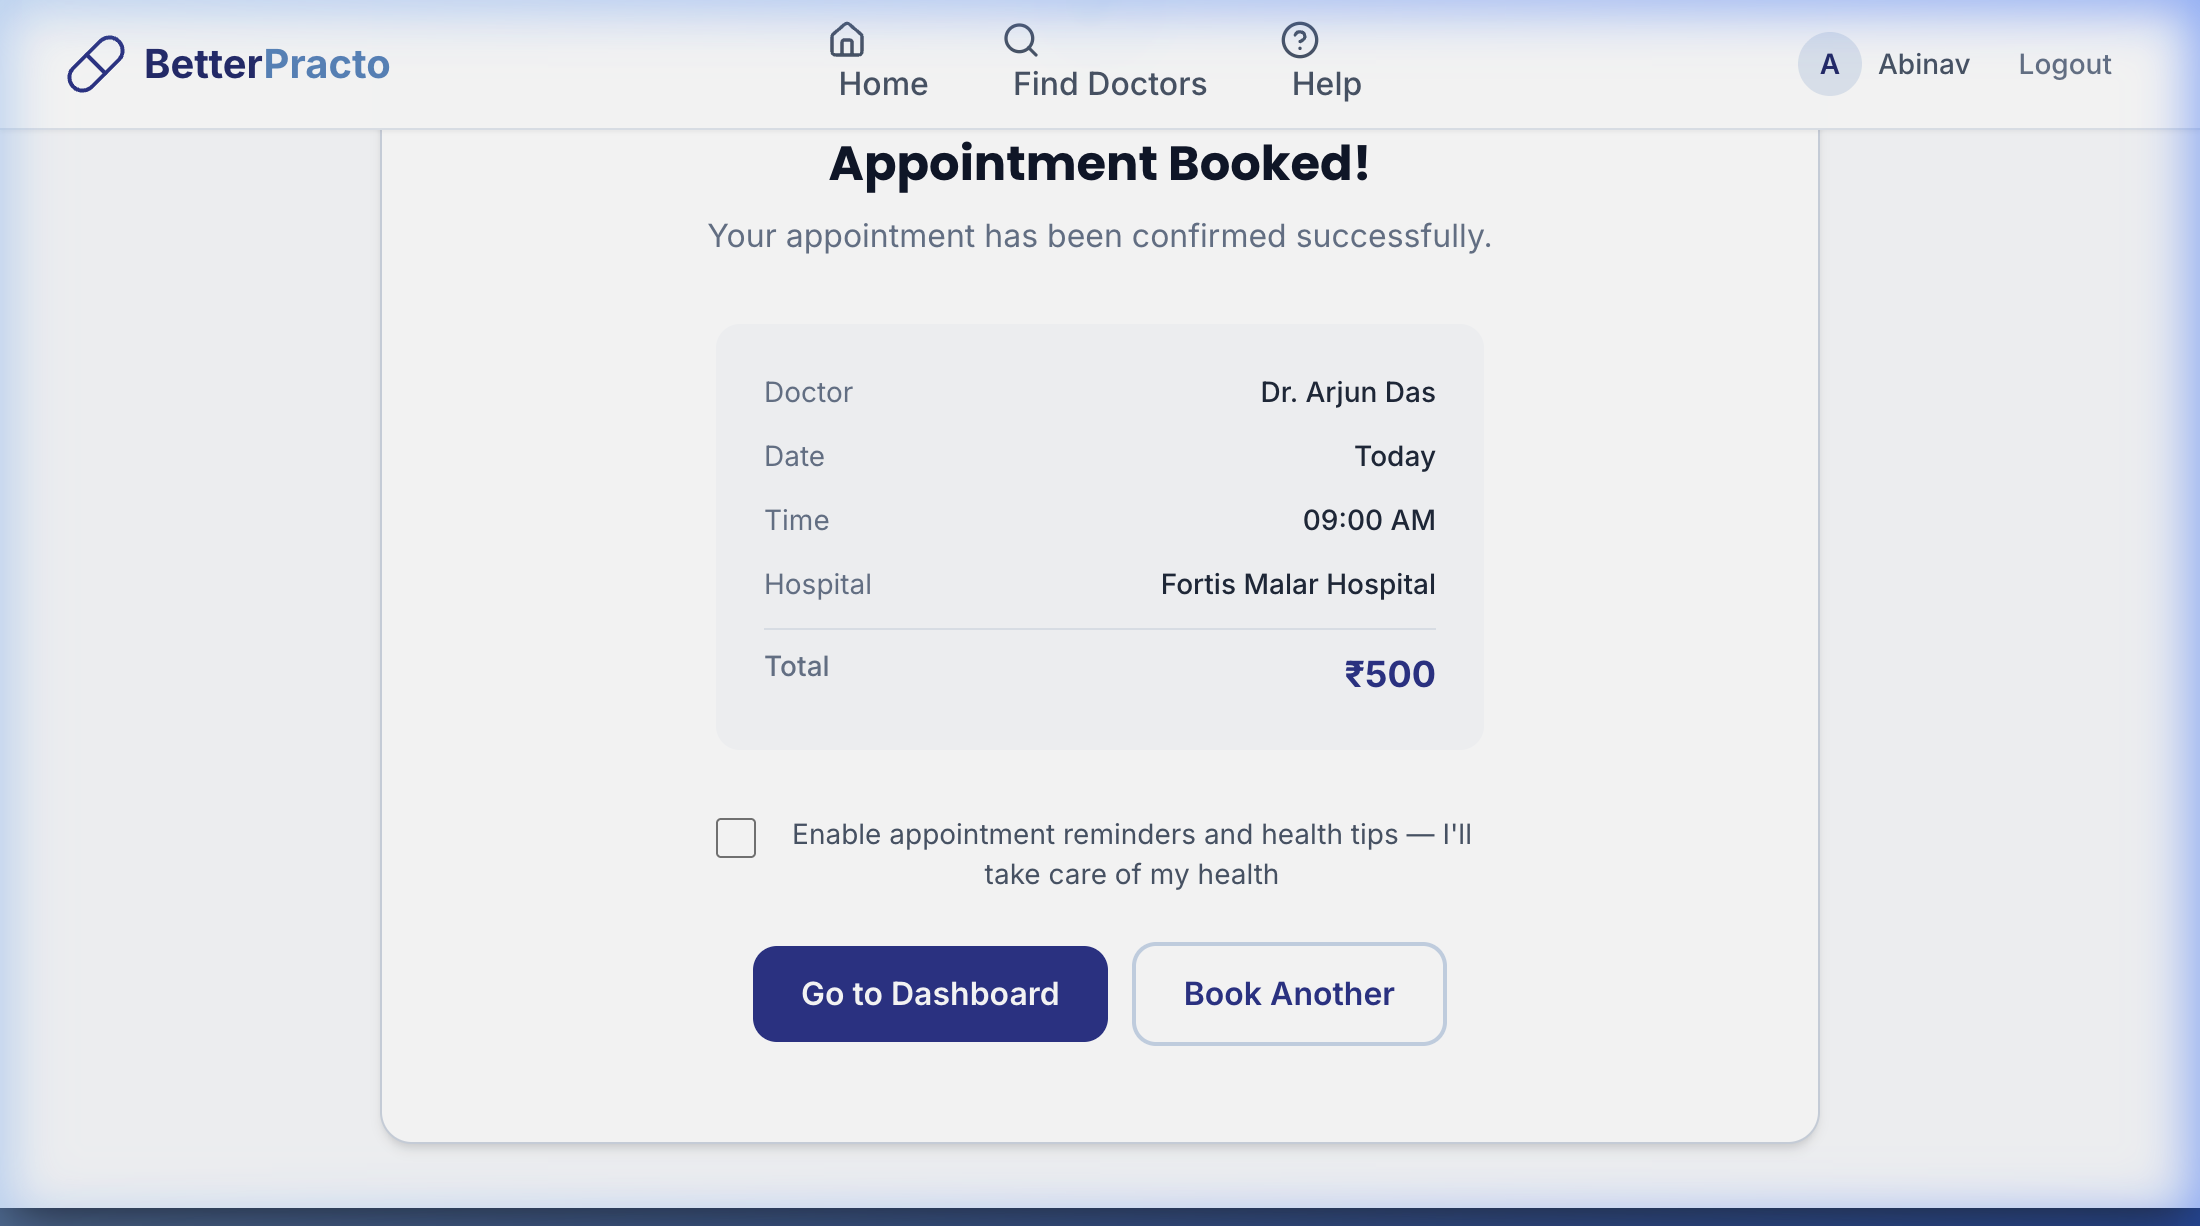
\includegraphics[width=\textwidth]{persuasion_commitment.png}}
    \caption{Booking Step 3 Success --- C5 Commitment: ``Enable appointment reminders'' checkbox below the booking summary. Booking is confirmed \emph{before} the checkbox appears, so it is never a blocker. \textit{Block C.}}
\end{figure}

\begin{figure}[H]
    \centering
    \imgborder{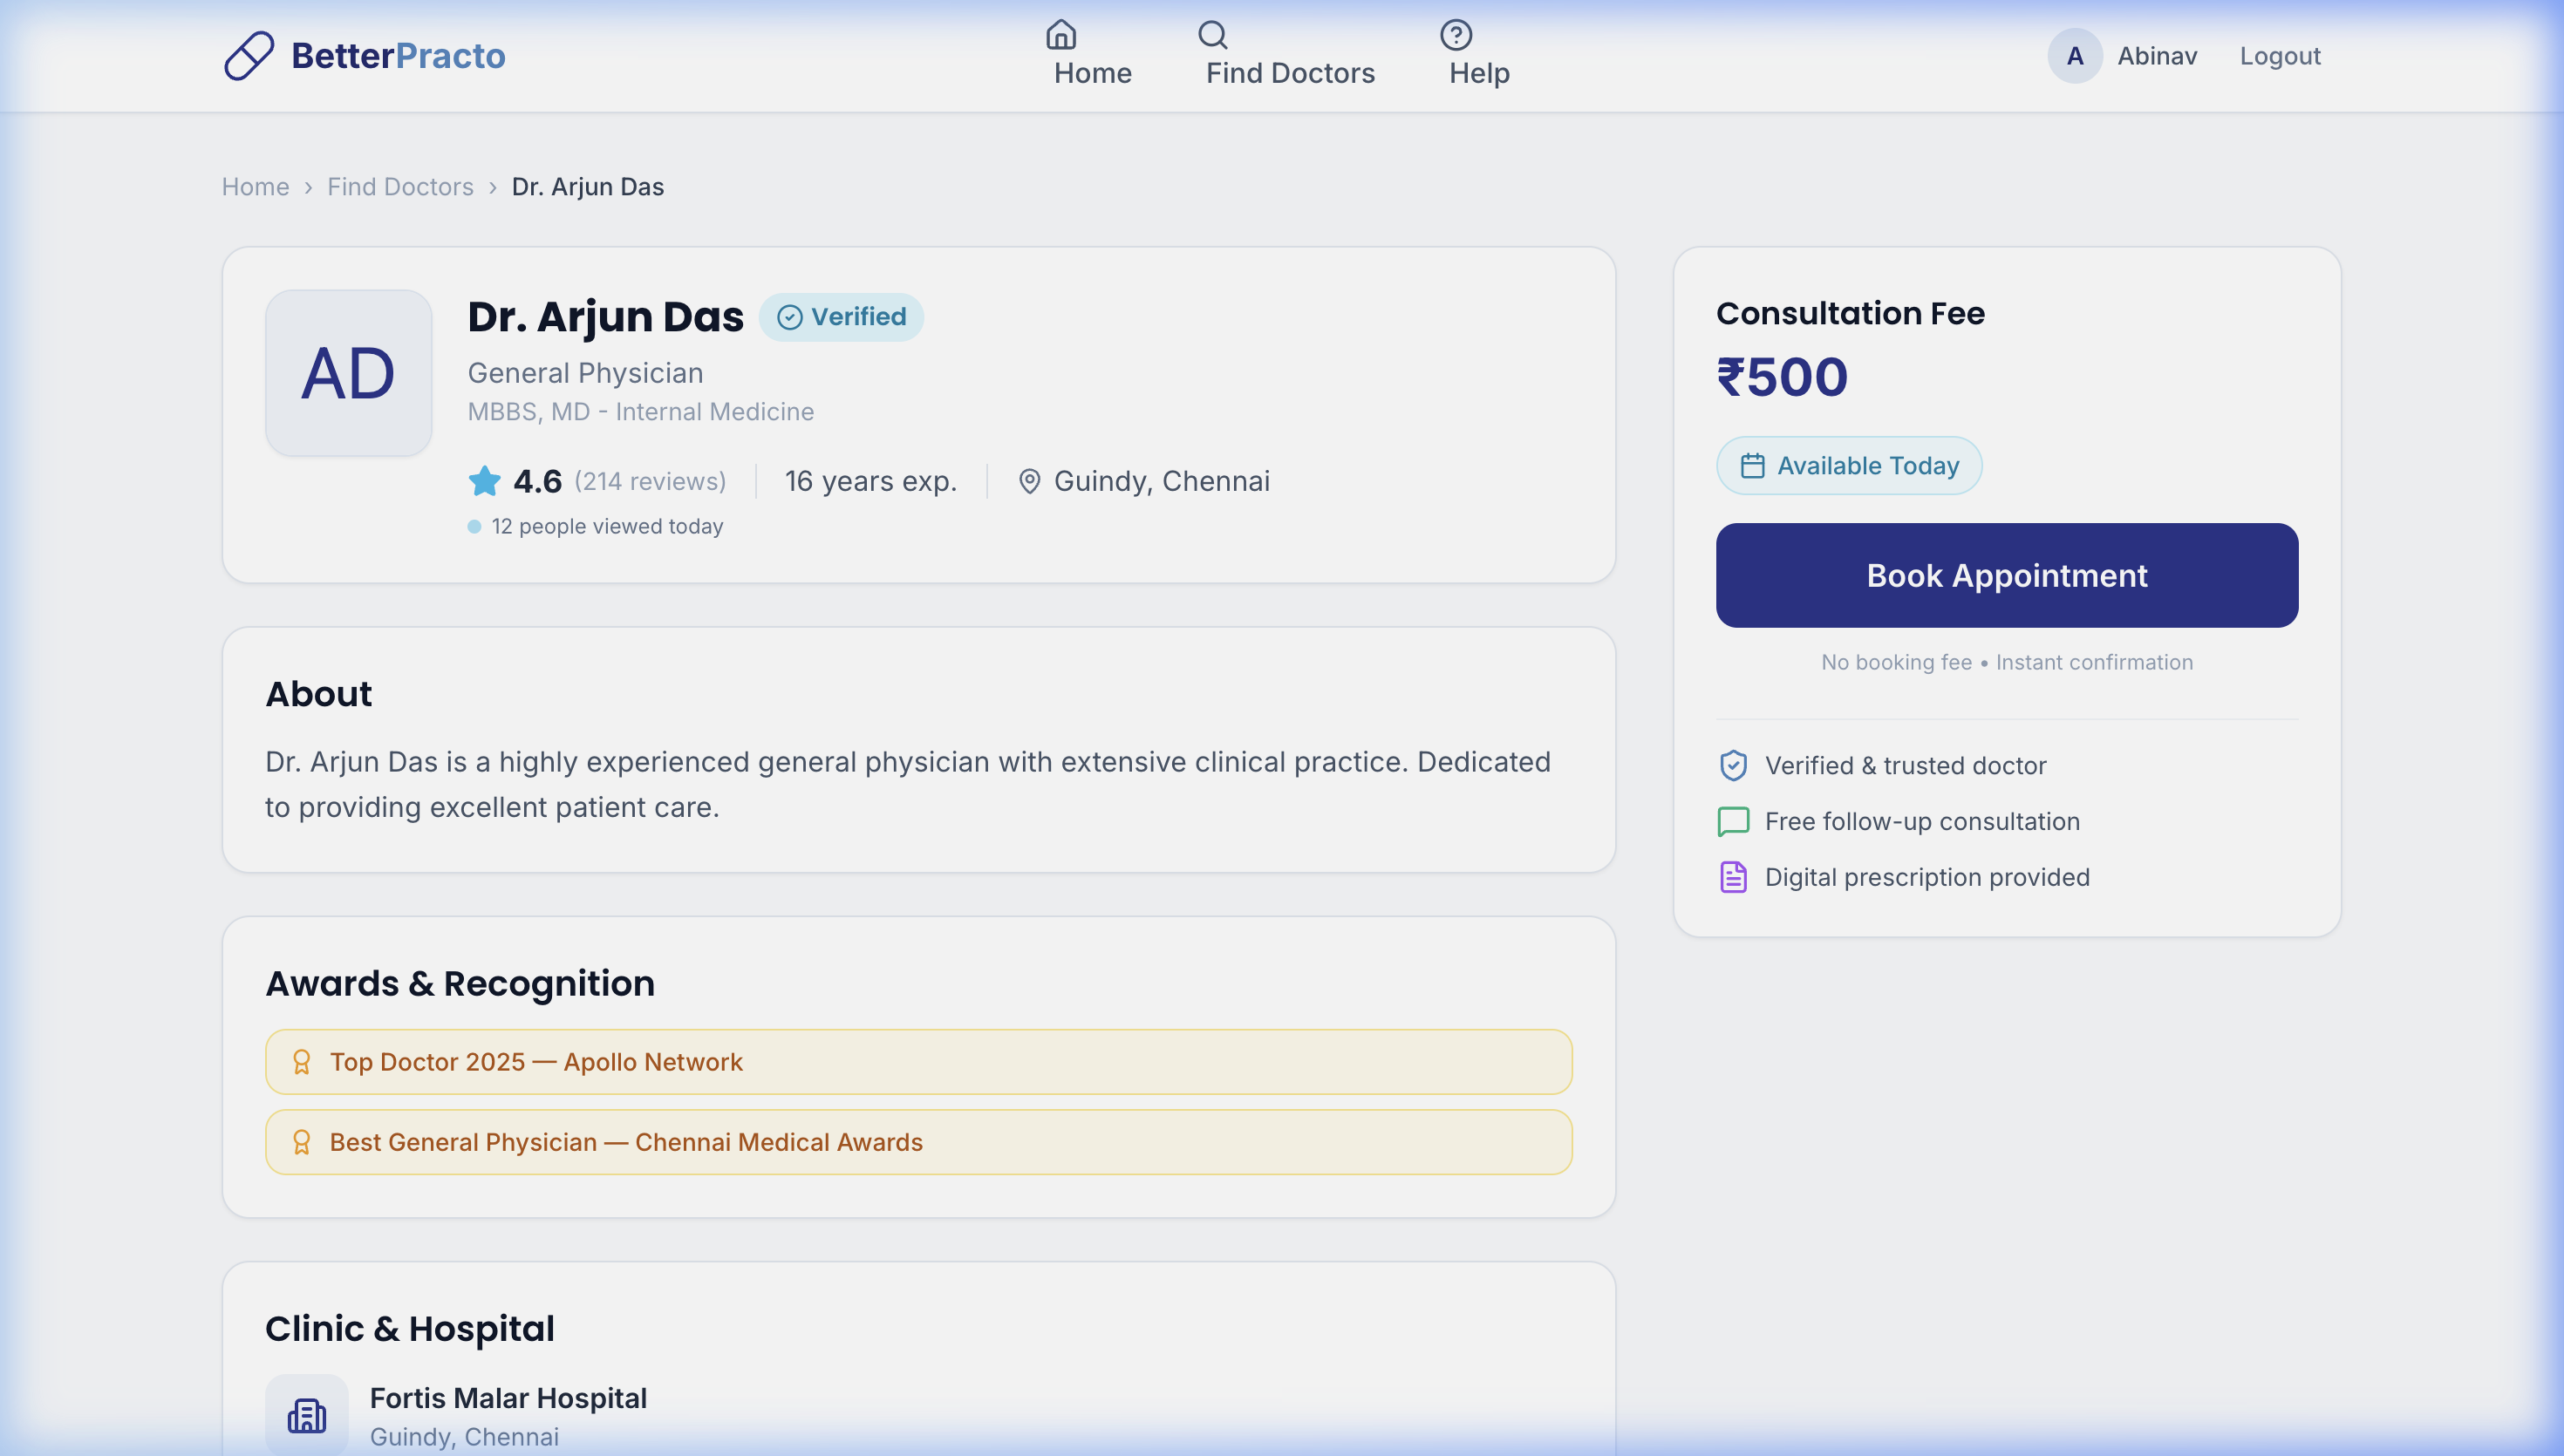
\includegraphics[width=\textwidth]{persuasion_authority.png}}
    \caption{Doctor Profile --- C1 Authority (amber award badges) and C2 Social Proof (``X people viewed today'' pulse dot). \textit{Block C.}}
\end{figure}

\vspace{0.5cm}

% =================================================================
\section{Block D --- Color \& Shape Psychology}
% =================================================================

\begin{hcibox}{Color Psychology \& Shape Psychology}
Color carries pre-attentive, culturally-mediated meaning. Shape communicates affordance and personality. Together, consistent color + shape systems reduce cognitive load by allowing users to decode meaning before reading.
\end{hcibox}

\subsubsection{Color Psychology Rationale (Better Practo palette)}

\begin{center}
\begin{tabular}{>{\bfseries}l l l}
\toprule
Color & Hex & Psychological Meaning \\
\midrule
Primary Blue & \#2A348C & Trust, calm, authority (Facebook, VISA, NHS) \\
Accent Cyan & \#14BEF0 & Fresh, innovative, approachable --- medical/digital \\
Trust Slate & \#64748b & Neutral, professional --- used for body text \\
Emerald & \#059669 & Natural, growth, health (Spotify, NHS green) \\
Amber & \#D97706 & Optimism, caution, visibility (DHL, McDonald's) \\
Red & \#DC2626 & Energy, danger, urgency (Coca-Cola, YouTube) \\
\bottomrule
\end{tabular}
\end{center}

\vspace{0.3cm}

\begin{figure}[H]
    \centering
    \begin{subfigure}[b]{0.47\textwidth}
        \imgborder{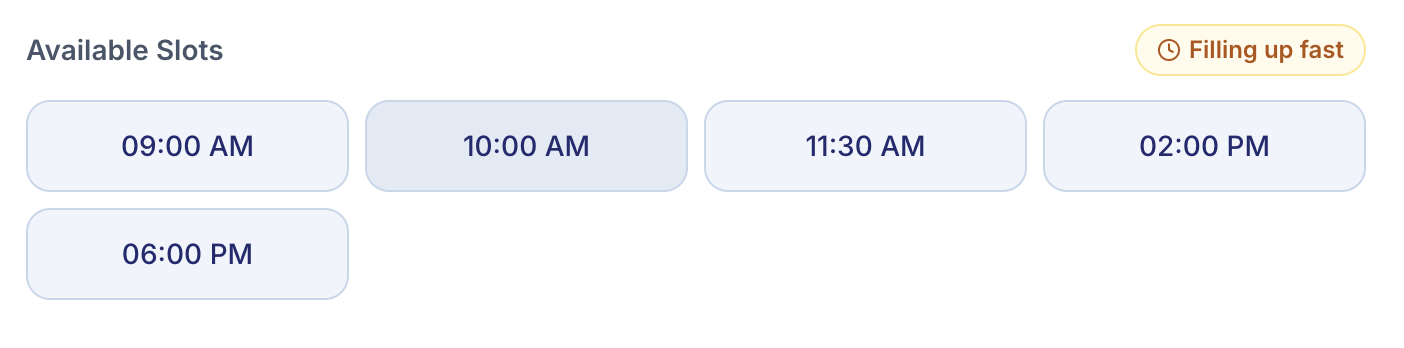
\includegraphics[width=\textwidth]{color_psychology_1.png}}
        \caption{Amber slots signal ``Filling up fast'' (urgency/caution).}
    \end{subfigure}
    \hfill
    \begin{subfigure}[b]{0.47\textwidth}
        \imgborder{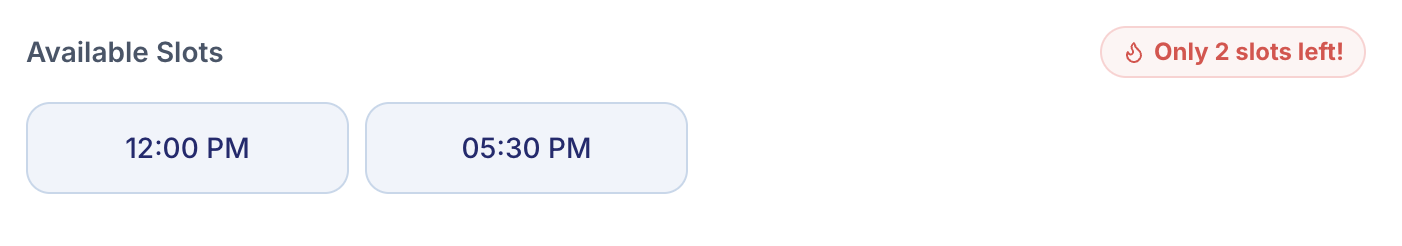
\includegraphics[width=\textwidth]{color_psychology_2.png}}
        \caption{Green slots signal ``Available'' (health/safe).}
    \end{subfigure}
    \caption{Color Psychology (Block D) in action on the Booking page. Meaning is conveyed through color before text is even read.}
\end{figure}

\vspace{0.3cm}

\subsubsection{Shape Psychology Rationale}

\begin{center}
\begin{tabular}{>{\bfseries}l l}
\toprule
Shape & Psychological Signal \\
\midrule
\texttt{rounded-xl} (12px) on primary buttons & Friendly, approachable, safe \\
\texttt{rounded-full} on pill badges & Soft, inclusive, non-threatening \\
Circular avatars & Completeness, unity (Gestalt Closure) \\
Square-edged data tables & Precision, authority, structure \\
\bottomrule
\end{tabular}
\end{center}

\vspace{0.5cm}

% =================================================================
\section{Block E --- User Support Systems}
% =================================================================

\begin{hcibox}{User Support Systems}
User support systems are classified by the type of user need they serve (Dix et al., 2004): \textbf{Quick Reference} (scannable cheat sheet for users who already know the system), \textbf{Task-Specific Help} (contextual guidance tied to the current action), \textbf{Full Explanation} (complete manual), \textbf{Tutorial} (step-by-step guidance for beginners), \textbf{Context-Sensitive Help} (automated, appears where needed), and \textbf{Adaptive Help} (adjusts to user expertise). Clippy (Microsoft Word 1997) is the canonical example of a \emph{failed} assistant: intrusive, irrelevant, blocks workflow.

\textit{Reference: End-Sem HCI Lecture Notes, lines 299--425.}
\end{hcibox}

\subsection{E1 --- Quick Reference Card}

\begin{featurebox}{Quick Reference --- Scannable Cheat Sheet on Help Page}
The Help page now opens with a ``QUICK REFERENCE --- Common Actions'' card \emph{above} the FAQ search bar. This implements the \textbf{Quick Reference} type of user support (Dix, 2004): a scannable, at-a-glance summary of the 4 most common user tasks with their navigation paths.

\textbf{Design rationale:}
\begin{itemize}[leftmargin=1.5em, itemsep=0pt]
  \item \textbf{Placed first (Primacy):} Serial Position Effect --- the first item on a page is remembered best. Experienced users who just need a reminder find it immediately without scrolling.
  \item \textbf{2×2 grid layout:} Parallel structure (Similarity) makes the 4 action paths instantly scannable --- no reading required.
  \item \textbf{Coloured icons:} Pre-attentive coding (Search=blue, Book=green, Video=blue, Help=purple) matches the colours used elsewhere in the app (Gestalt Similarity).
  \item \textbf{Dark blue header:} Visual Dominance (Block B) --- the Quick Reference is the most visually prominent element on the page, ensuring it is seen first.
\end{itemize}

This contrasts sharply with Practo's help page (violation V6) which has no Quick Reference and forces all users --- including experienced ones --- to search through FAQs or use the search bar.

\textit{Implementation: \texttt{src/pages/Help.jsx}, above the FAQ search bar.}
\end{featurebox}

\begin{figure}[H]
    \centering
    \imgborder{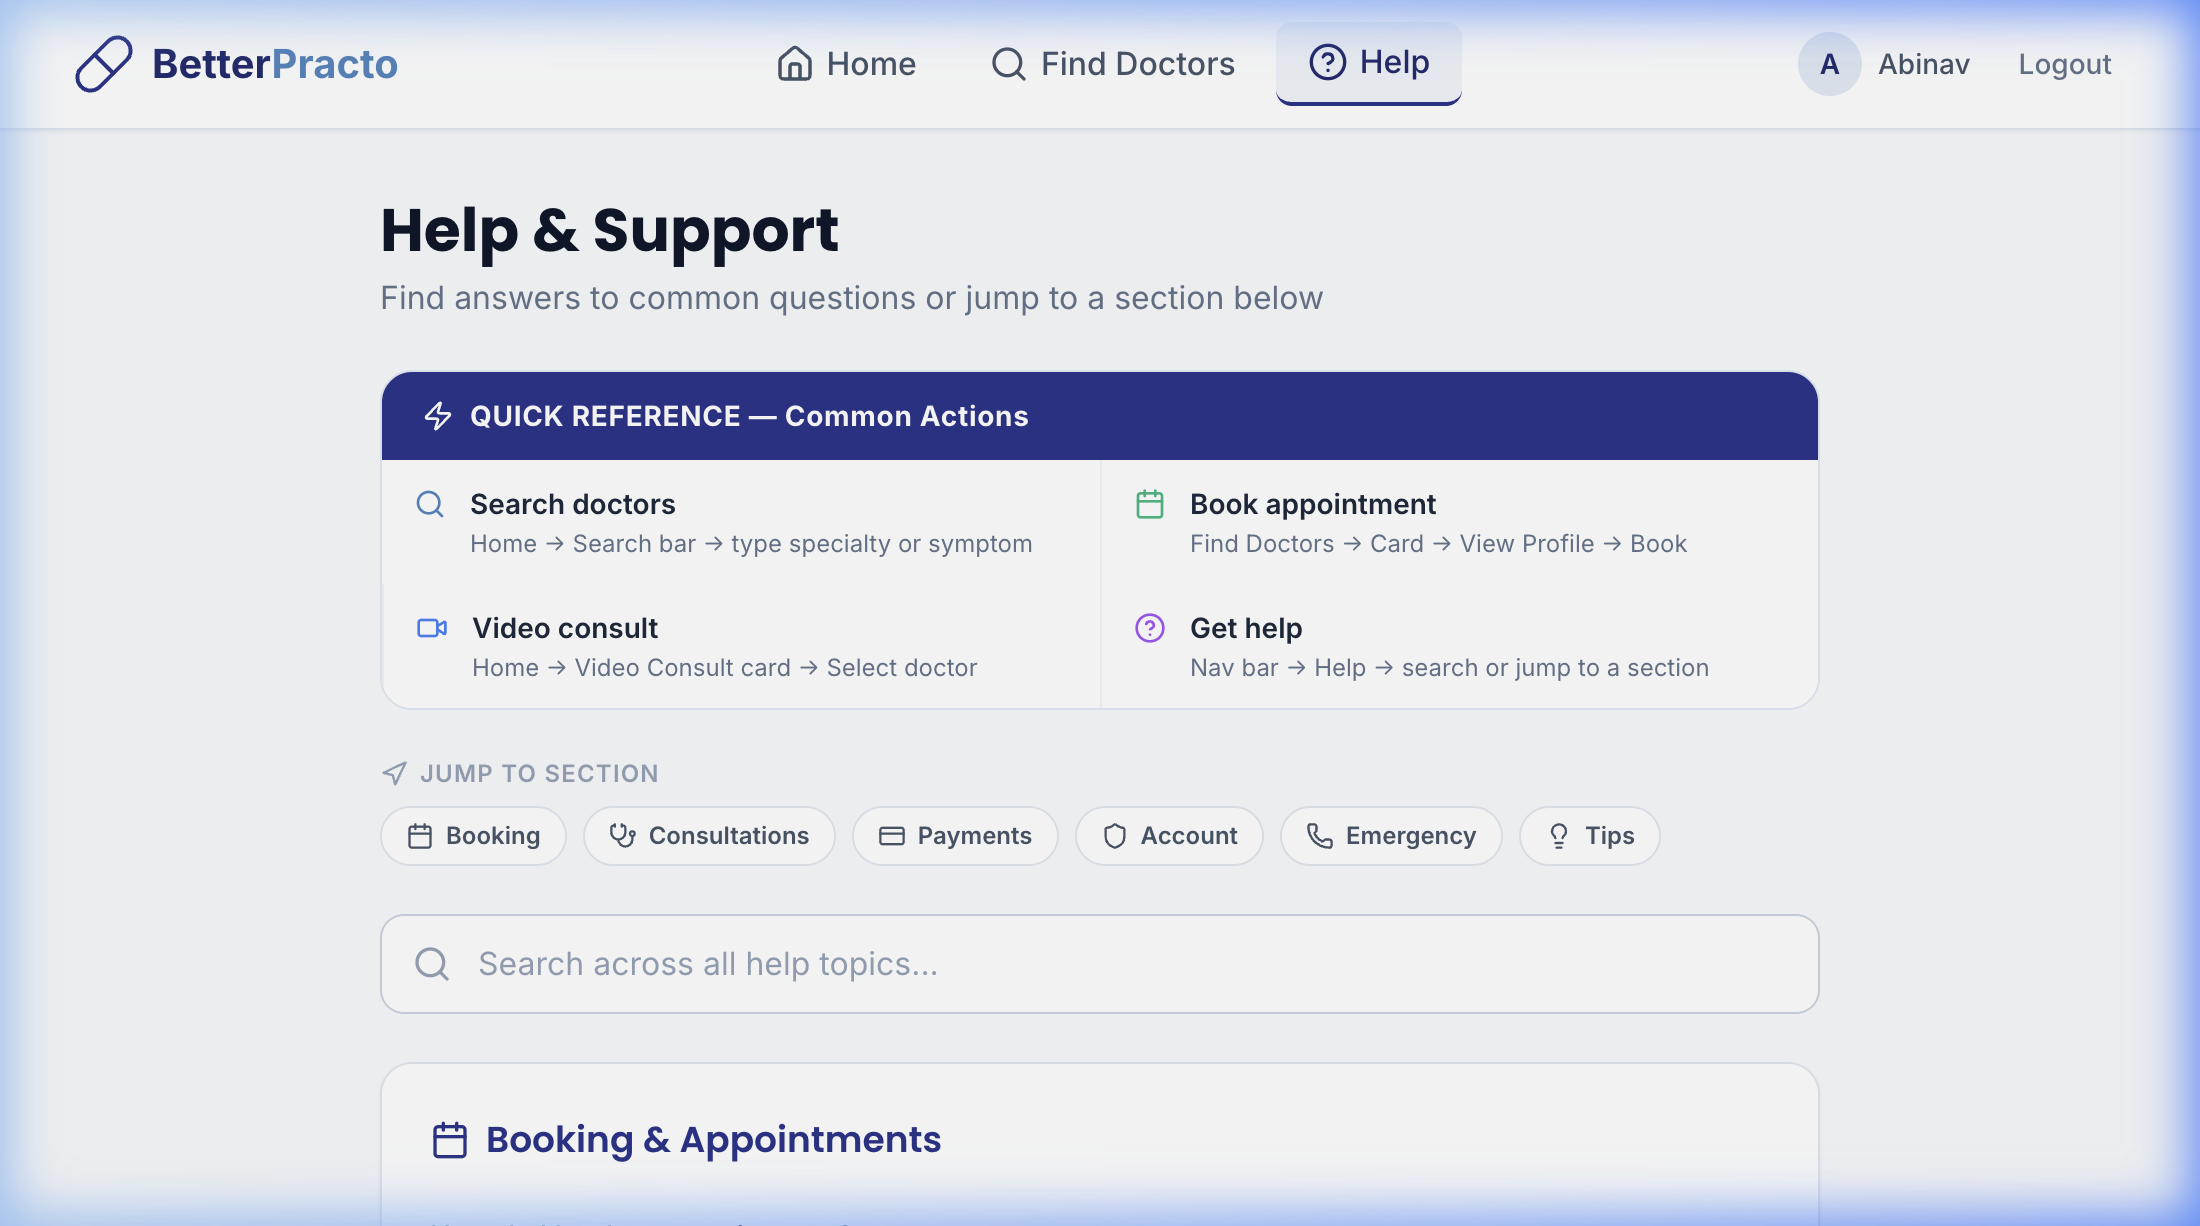
\includegraphics[width=\textwidth]{user_support_quickref.png}}
    \caption{Help page: E1 Quick Reference card (dark blue header + 2\texttimes{}2 action grid) above the Jump-to-section pills, FAQ search bar, and FAQ accordion. Experienced users find common tasks instantly; novices use the FAQ. \textit{Block E.}}
\end{figure}

\subsection{E2 --- Tips \& Best Practices (Proactive Help)}

\begin{featurebox}{Proactive Help --- Tips \& Warnings Panel}
Dix et al.\ (2004) describe proactive help as assistance that anticipates user problems \emph{before} they occur, rather than waiting for errors. The Help page now includes a 2\texttimes{}2 ``Tips \& Best Practices'' grid with actionable warnings: book 24h in advance, bring test reports, ensure stable internet for video, enable reminders. Each tip uses a coloured icon (blue=info, green=health, purple=tech, orange=action) matching the rest of the app's colour system (Block D).
\end{featurebox}

\subsection{E3 --- Emergency Contact Card (Always Visible System Support)}

\begin{featurebox}{Emergency Contacts --- Safety Net for Critical Situations}
A red-themed ``Emergency Contacts'' card is always visible near the bottom of the Help page, showing: Ambulance (108), National Health Helpline (104), and 24/7 in-app support chat. This implements the \textbf{Tolerance for Error} principle (Universal Design, Block I) at the information architecture level: a user in a health emergency who accidentally navigates to the Help page is immediately shown the correct exit path. This can be life-critical --- the design ensures it is unmissable (red background, prominent number).
\end{featurebox}

\begin{figure}[H]
    \centering
    \imgborder{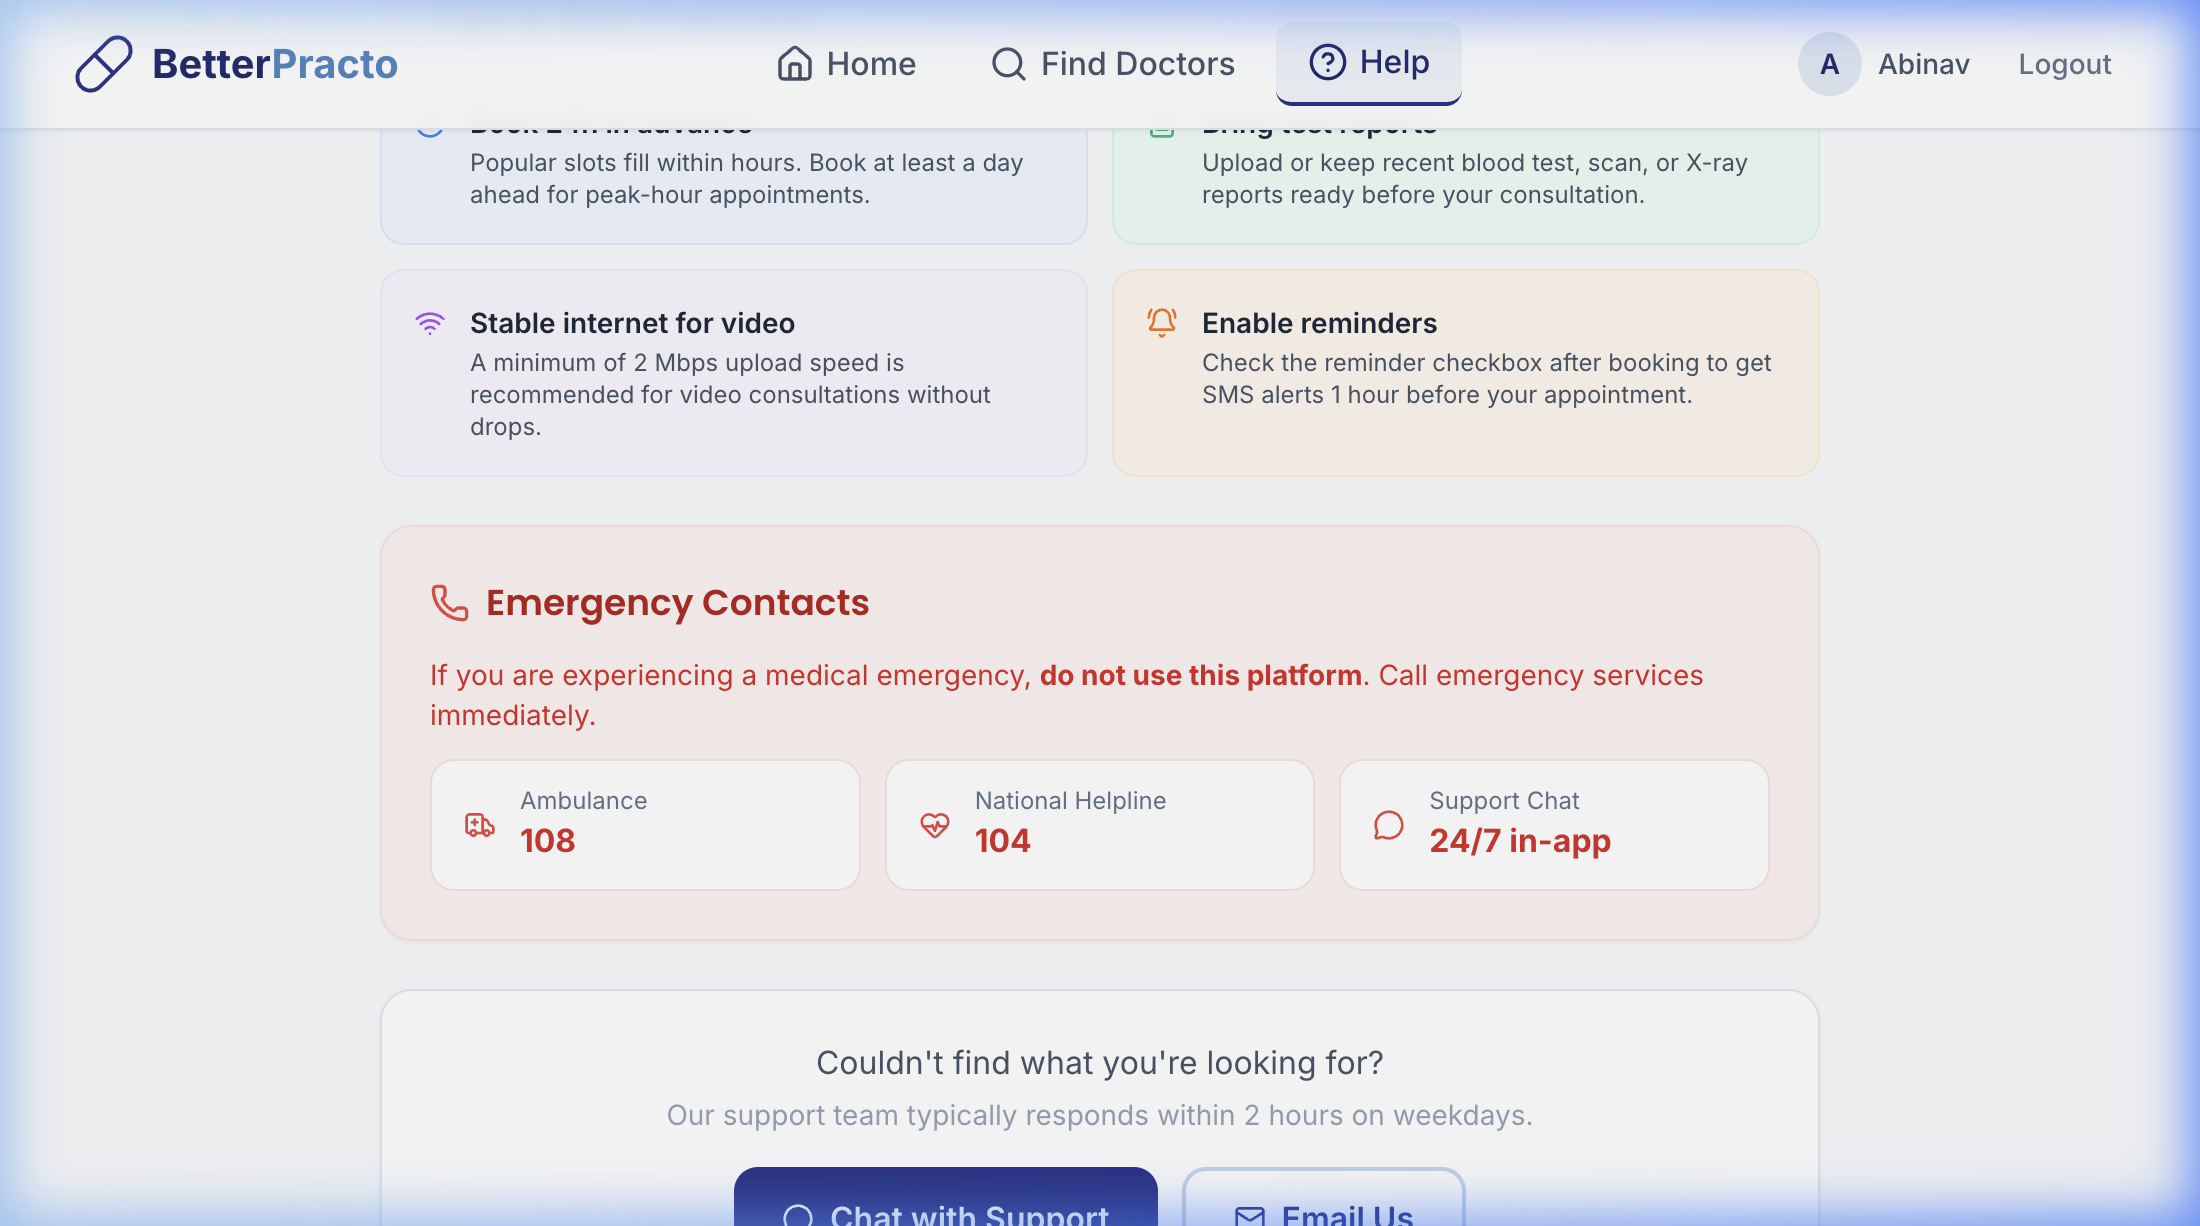
\includegraphics[width=\textwidth]{help_emergency.png}}
    \caption{Bottom of Help page: E2 Tips \& Best Practices (2\texttimes{}2 coloured grid) and E3 Emergency Contacts card (red, with 108/104 numbers). Couldn't find help? → Chat or Email buttons below. \textit{Block E.}}
\end{figure}

\vspace{0.5cm}

% =================================================================
\section{Block F --- Navigation Design Guidelines}
% =================================================================

\begin{hcibox}{Navigation Design Guidelines}
Key navigation principles (Web Usability lecture): every page must show the user \emph{where they are}, \emph{where they can go}, and \emph{where they have been}. Breadcrumbs satisfy all three. Skip navigation links allow keyboard and screen-reader users to bypass the repeated nav bar and jump directly to main content --- required by WCAG 2.1 Success Criterion 2.4.1.
\end{hcibox}\subsection{F1 --- Keyboard Navigation Toast}

\begin{featurebox}{Keyboard Navigation Toast --- Non-Intrusive Keyboard Mode Indicator}
The previous implementation used a full-width banner that covered the navbar --- a poor design choice that obstructed the primary navigation. The redesigned F1 feature works as follows:
\begin{itemize}[leftmargin=1.5em, itemsep=0pt]
  \item A \texttt{useEffect} in \texttt{Navbar.jsx} listens for the first \texttt{Tab} keydown event on the window.
  \item On first Tab press, a dark-blue toast appears in the \textbf{bottom-right corner} (\texttt{fixed bottom-6 right-6 z-[200]}), reading: ``Keyboard navigation active --- use Tab to move between elements''.
  \item The toast auto-dismisses after 3 seconds and has an \texttt{\texttimes} button for immediate dismissal.
  \item A \texttt{role="status" aria-live="polite"} attribute ensures screen readers announce it without interrupting other content.
  \item Mouse users never see it. It fires only once per session.
\end{itemize}

\textit{Why a toast, not a banner?} A banner that covers the navbar is an Anti-Pattern --- it obstructs the primary navigation while trying to help keyboard users navigate. A bottom-right toast follows the Notification UX convention (familiar from Gmail, Figma, VS Code) and does not block any content.
\end{featurebox}

\subsection{F2 --- In-Page Jump Navigation on Help Page}

\begin{featurebox}{In-Page Jump Navigation --- Visible Skip-Link Concept}
The Help page implements a visible, interactive ``Jump to section'' pill row below the Quick Reference card. Six section pills (Booking, Consultations, Payments, Account, Emergency, Tips) allow users to:\begin{itemize}[leftmargin=1.5em, itemsep=0pt]
  \item Jump directly to any section with \texttt{scrollIntoView\{behavior: smooth\}} --- bypassing all content in between (the visible equivalent of a skip link).
  \item The active section pill changes to a filled primary style, giving location feedback (Nielsen \#1: Visibility of System Status / navigation principle ``Where am I?'').
  \item Each section card has \texttt{id} attributes matching the pills, and \texttt{scroll-mt-20} to offset the sticky navbar.
\end{itemize}

This is the \textbf{visible, user-friendly implementation} of the skip-link concept. While WCAG skip links are invisible by default (keyboard-only), the Jump Navigation makes the same concept accessible to all users.
\end{featurebox}

\subsection{F3, F4 --- ARIA Labels + Keyboard-Navigable Logo}

\begin{featurebox}{ARIA Labels + Keyboard Navigation}
\textbf{F3 --- \texttt{aria-label} on \texttt{\textless{}nav\textgreater{}:}} The navbar element has \texttt{aria-label="Primary navigation"}, allowing screen-readers to identify this landmark region.

\textbf{F4 --- Logo keyboard-navigable:} The logo has \texttt{role="link"}, \texttt{tabIndex=\{0\}}, \texttt{aria-label="Go to home page"}, and \texttt{onKeyDown} Enter handler. The mobile menu button has \texttt{aria-expanded} set dynamically.
\end{featurebox}

\subsection{F5 --- Breadcrumb Navigation}

\begin{featurebox}{Breadcrumb Navigation --- Synthesizability}
The DoctorProfile and Booking pages show breadcrumbs: \texttt{Home \textrightarrow{} Find Doctors \textrightarrow{} Dr. [Name]} and \texttt{Home \textrightarrow{} [Doctor] \textrightarrow{} Book Appointment}. Satisfies: \textit{where am I? where have I been? where can I go?}
\end{featurebox}

\begin{figure}[H]
    \centering
    \imgborder{
\includegraphics[width=\textwidth]{navigation_breadcrumb.png}}
    \caption{Breadcrumb navigation providing synthesizability: the user knows their location, path, and can step backwards. \textit{Block F.}}
\end{figure}

\begin{figure}[H]
    \centering
    \imgborder{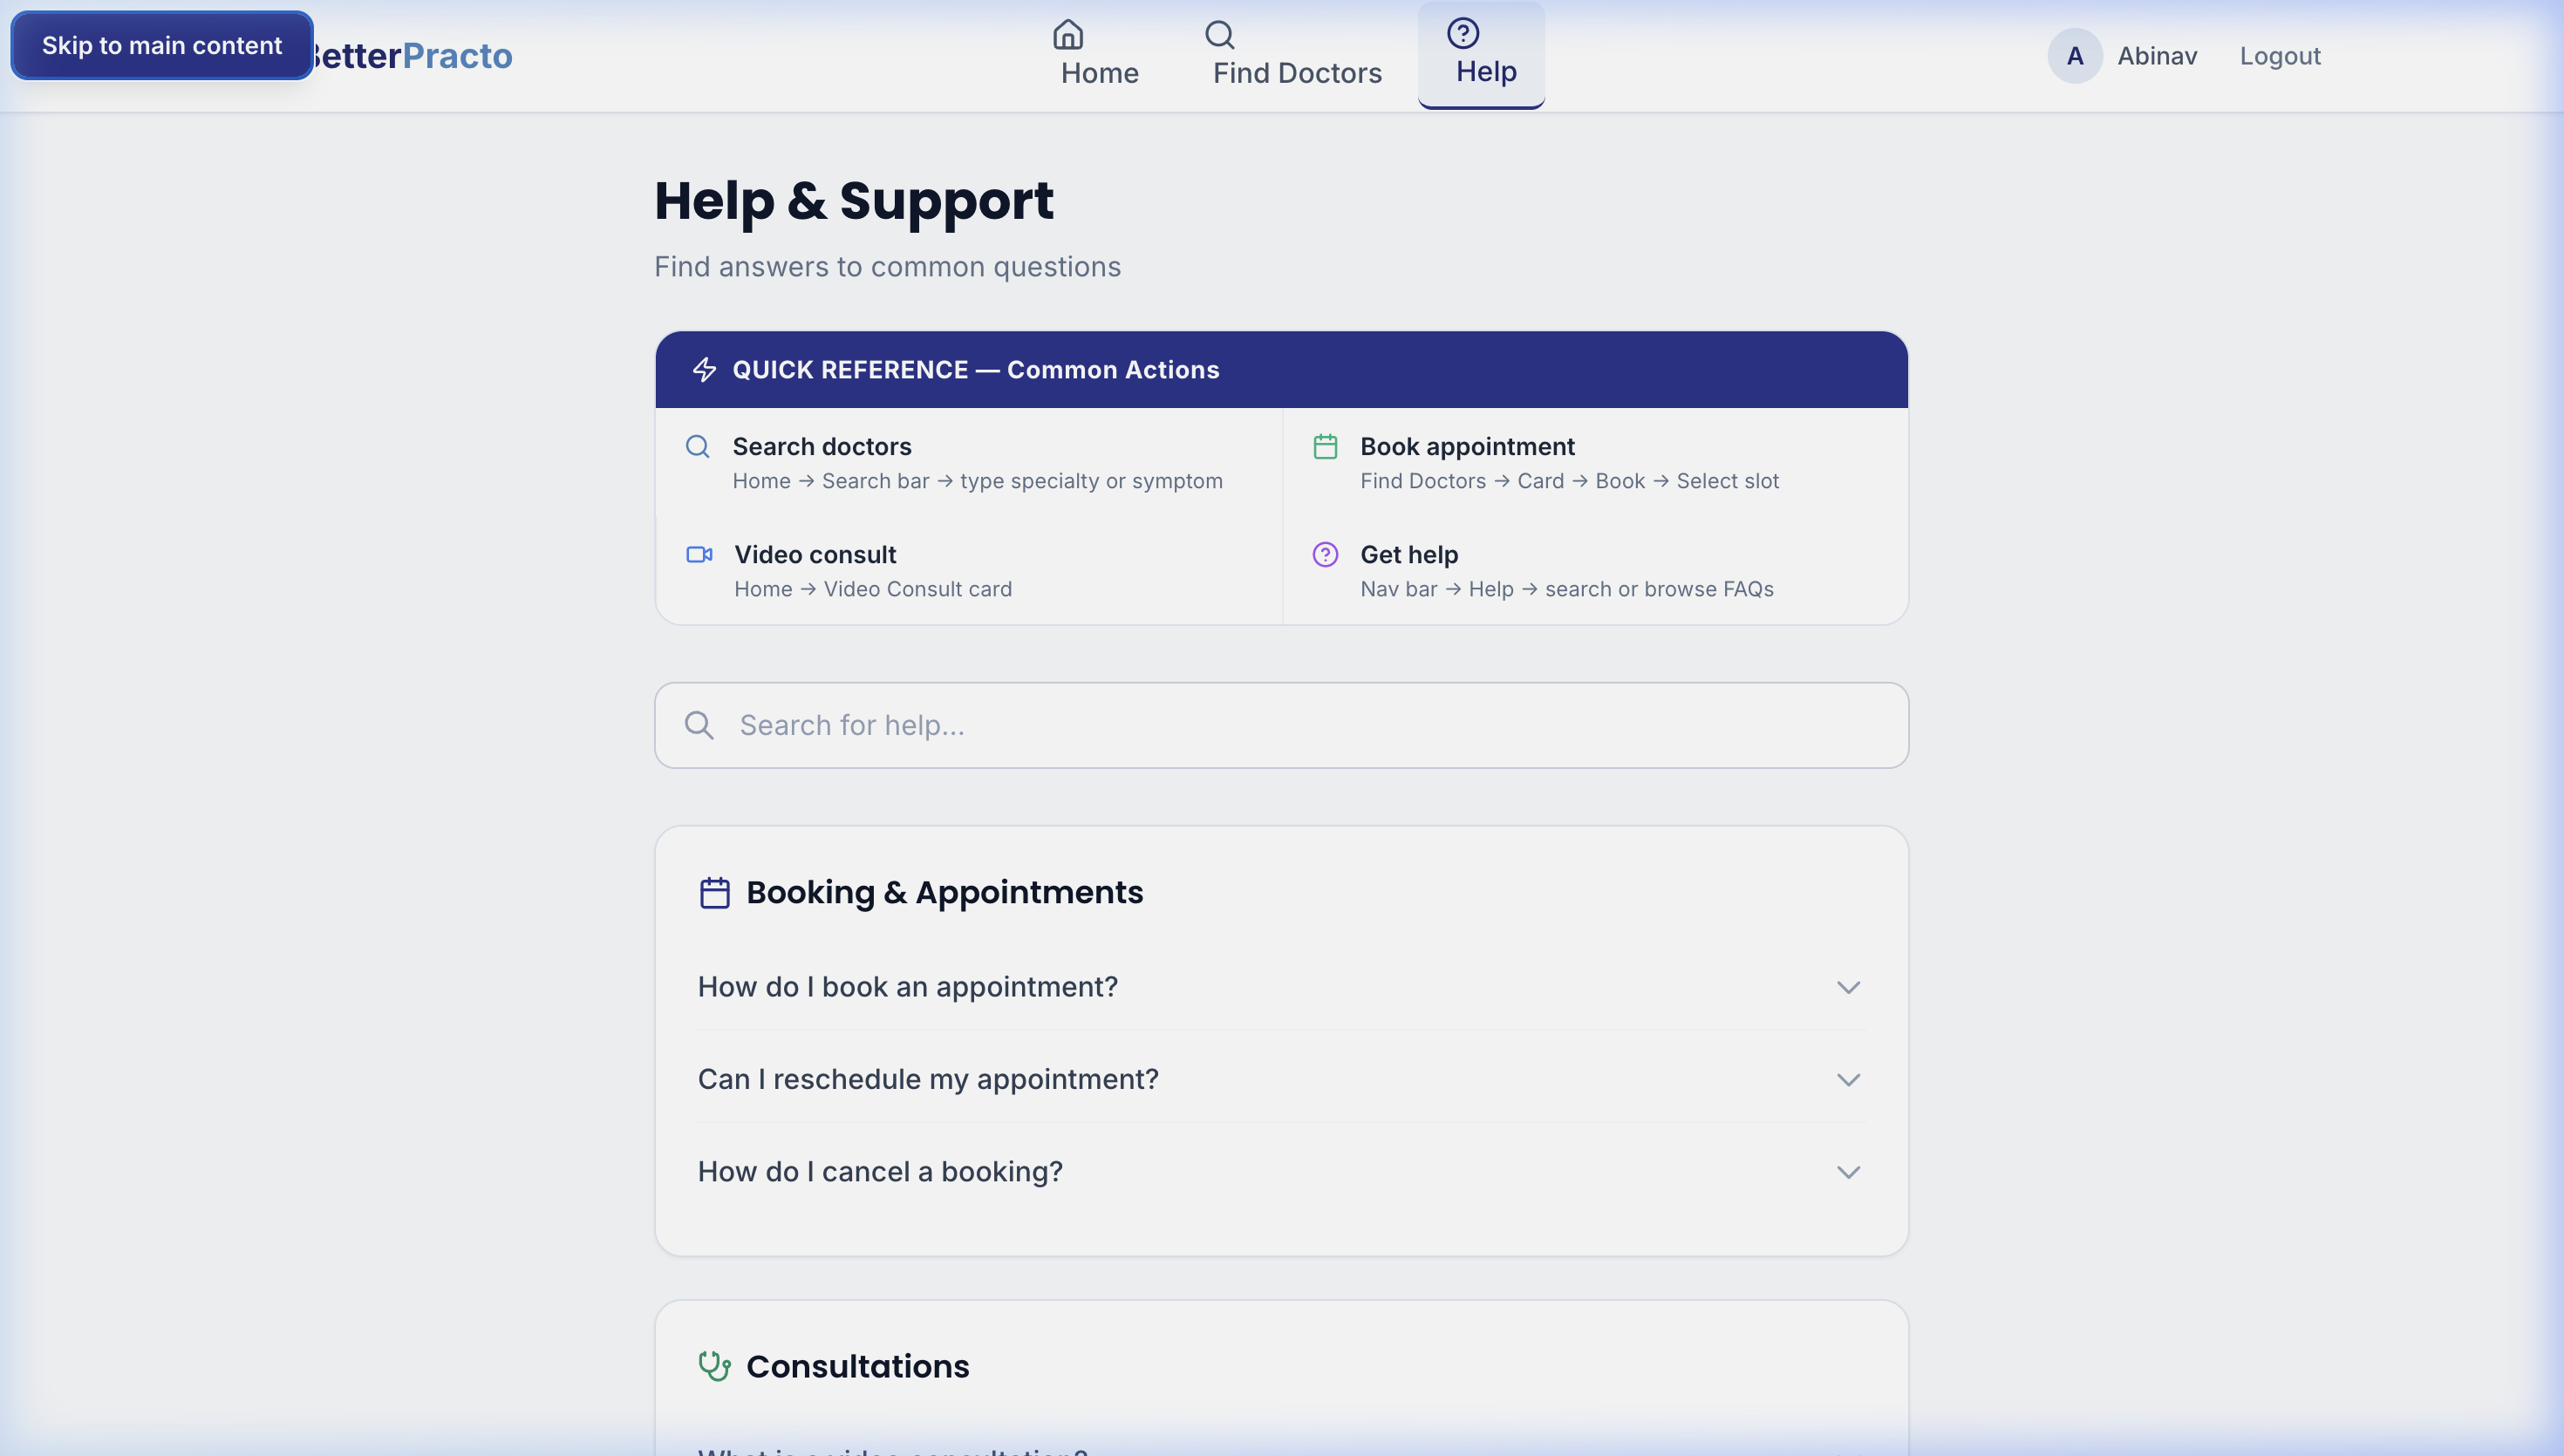
\includegraphics[width=\textwidth]{navigation_skip_link.png}}
    \caption{Help page showing F2 Jump-to-section pill row (``Booking'' active, filled blue; others outlined) and F1 keyboard toast appearing in bottom-right after Tab key press: ``Keyboard navigation active --- use Tab to move between elements''. \textit{Block F.}}
\end{figure}

\vspace{0.5cm}

% =================================================================
\section{Block H --- Web Usability Guidelines}
% =================================================================

\begin{hcibox}{Web Usability Guidelines --- Krug's ``Don't Make Me Think''}
Steve Krug's central law: every question mark in the user's mind adds cognitive friction and undermines trust. Applied principles: \textbf{Feature Exposure} (make all capabilities visible), \textbf{Self-Evident Design} (actions and objects are immediately recognisable), \textbf{Graceful Degradation} (custom 404 page, not browser default), and \textbf{SEO Meta Tags} (OG tags, description, twitter:card --- web accessibility for search engines).

\\textit{Reference: End-Sem HCI Lecture Notes, lines 211--227.}
\end{hcibox}

\subsection{H1 --- Custom 404 Page (Graceful Degradation)}

\begin{featurebox}{Custom 404 Page --- Graceful Degradation}
The Web Usability Cheat Sheet (point 1, Accessibility) explicitly states: ``custom 404 page'' as a required accessibility feature. A browser-default 404 breaks the user's mental model --- they see a blank page with an error code and no path forward, violating both Nielsen \#9 (Help Users Recover from Errors) and Krug's Law (Don't Make Me Think).

The BetterPracto NotFound page (\texttt{src/pages/NotFound.jsx}) provides:
\begin{itemize}[leftmargin=1.5em, itemsep=0pt]
  \item \textbf{Visual clarity:} Large ``404'' in light grey text with an amber {\texttt{AlertTriangle}} icon overlay --- communicates the error immediately without alarming the user.
  \item \textbf{3 recovery paths:} Go Home (blue), Find Doctors (green), Help Page (purple) --- Feature Exposure principle: all app sections are visible at the moment the user is most disoriented.
  \item \textbf{``Go back'' link:} \texttt{navigate(-1)} takes the user to their previous page --- appropriate for users who mistyped a URL.
  \item \textbf{Navbar preserved:} The sticky navbar is still rendered above the 404, so the user can navigate normally.
\end{itemize}

\textit{Implementation:} \texttt{src/pages/NotFound.jsx} wired to the wildcard route \texttt{path="*"} in \texttt{App.jsx}.
\end{featurebox}

\subsection{H2 --- Chatbot Assistant (In-App User Support)}

\begin{featurebox}{Chatbot Assistant --- Unobtrusive Always-Available Support}
Reference (end\_sem\_reference.txt, §4 Assistants): \textit{``Assistants passively monitor user behaviour and offer suggestions when relevant. Ideally, they're unobtrusive and under user control. The infamous example is Microsoft's Clippy, which failed because it was intrusive and its suggestions were often irrelevant.''}

The \texttt{ChatbotAssistant} component (\texttt{src/components/ChatbotAssistant.jsx}) implements the \textbf{Assistants} type of user support with explicit anti-Clippy design decisions:

\begin{itemize}[leftmargin=1.5em, itemsep=0pt]
  \item \textbf{Non-intrusive FAB:} A 52$\times$52px dark-blue floating action button sits in the bottom-right corner. It never auto-opens, never interrupts, never animates beyond a single small red dot on first load.
  \item \textbf{User-controlled opening:} Click to open; the window appears as a smooth scale animation. Click $\times$ to dismiss. The background app remains fully interactive.
  \item \textbf{Quick-reply chips:} Each bot response includes 2--5 contextual chips for common follow-up queries --- supporting both novice users (chips) and experts (free text).
  \item \textbf{Typing indicator:} 3-dot bounce animation gives feedback that the bot is ``thinking'' --- Nielsen \#1: Visibility of System Status.
  \item \textbf{Keyword-matched FAQ knowledge base:} 10 intent categories (booking, cancel, payment, refund, video, account, privacy, doctors, emergency, greeting) cover the full app domain.
  \item \textbf{Emergency escalation:} Typing ``emergency'', ``108'', or ``urgent'' immediately surfaces ambulance and health helpline numbers --- a safety-critical feature.
  \item \textbf{\texttt{aria-live="polite"}:} Bot responses are announced to screen readers non-interruptively.
\end{itemize}
\end{featurebox}

\begin{figure}[H]
    \centering
    \begin{subfigure}[b]{0.47\textwidth}
        \imgborder{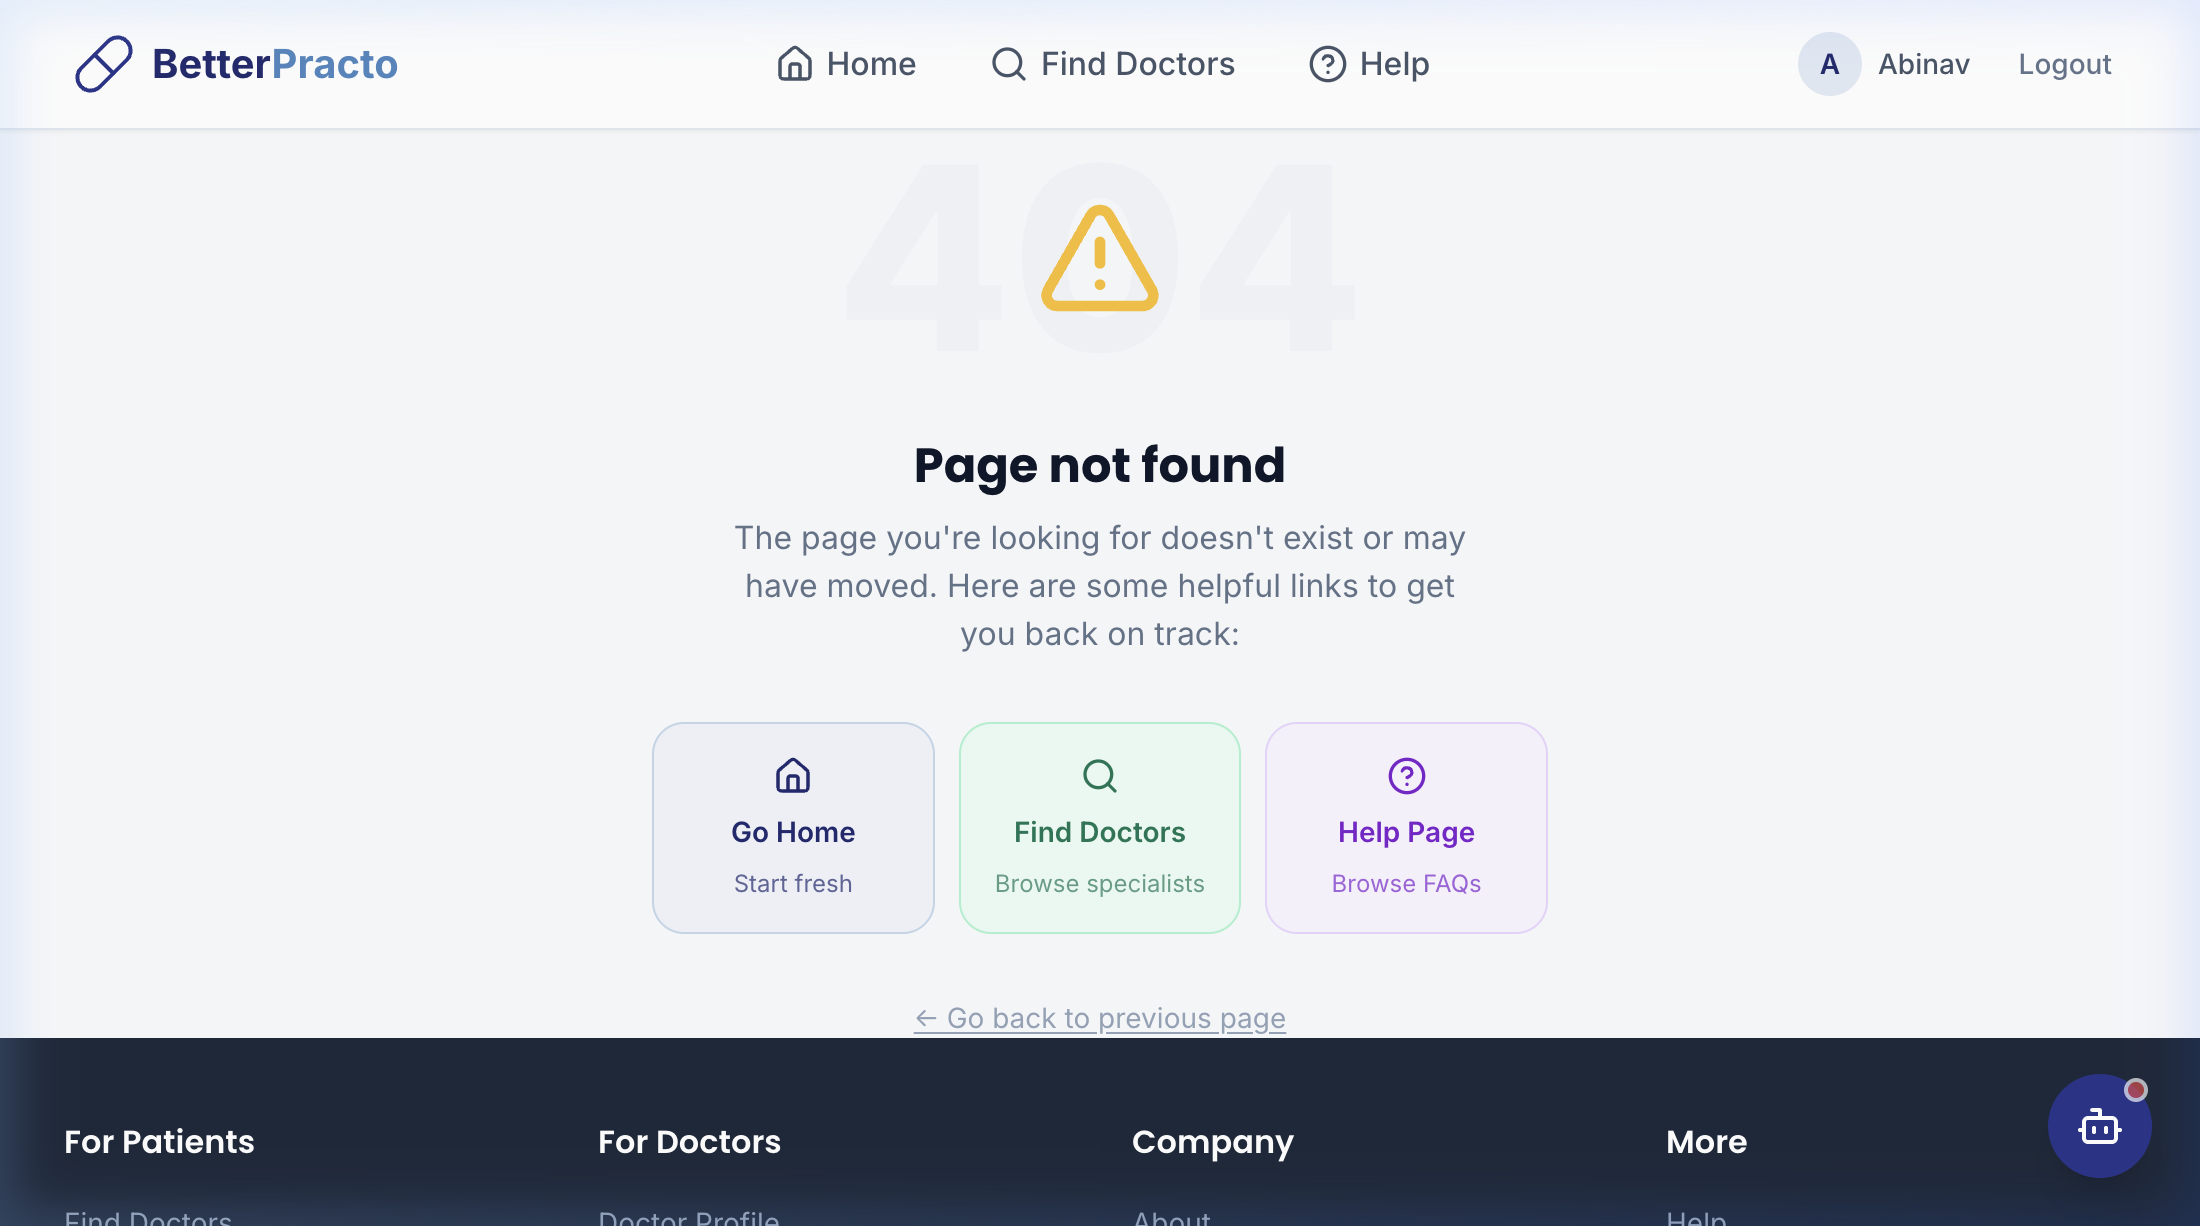
\includegraphics[width=\textwidth]{web_usability_404.png}}
        \caption{H1 Custom 404: amber triangle on faint ``404'', plain-language explanation, 3 colour-coded recovery cards, back link. Navbar still visible for orientation. \textit{Block H.}}
    \end{subfigure}
    \hfill
    \begin{subfigure}[b]{0.47\textwidth}
        \imgborder{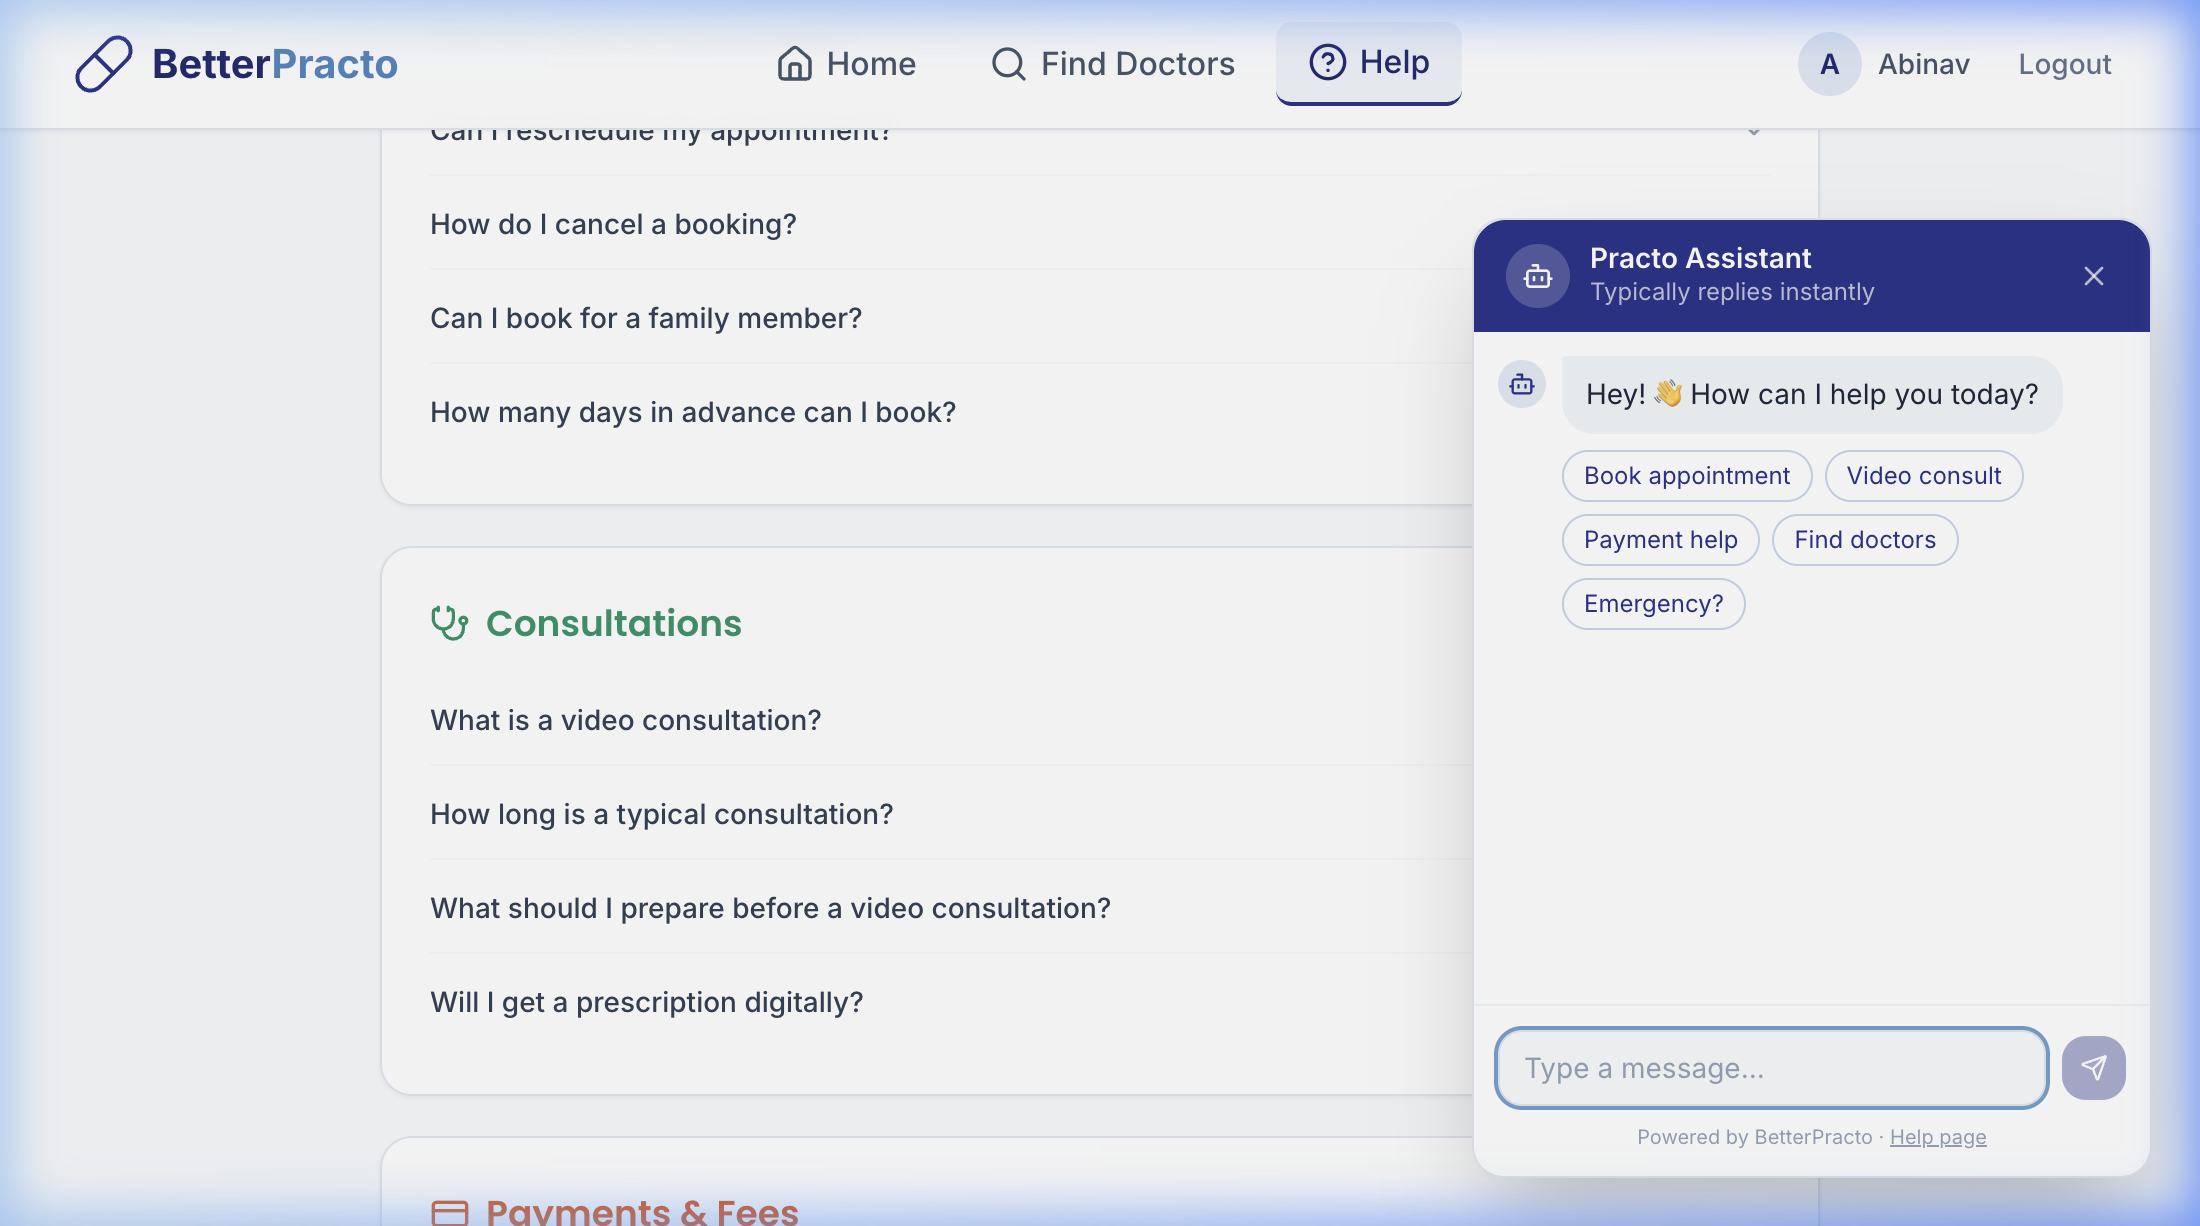
\includegraphics[width=\textwidth]{web_usability_chatbot_open.png}}
        \caption{H2 Chatbot open: dark-blue header, greeting, quick-reply chips. H3 visible context: FAQ accordion and chatbot coexist without interference. \textit{Block H.}}
    \end{subfigure}
\end{figure}

\subsection{H3 --- Efficiency of Use: Keyboard Shortcuts Modal}

\begin{featurebox}{Efficiency of Use --- Accelerators for Experts}
Nielsen's Heuristic \#7 (Flexibility and Efficiency of Use) states that accelerators may often speed up the interaction for the expert user. In Phase 7.5, global keyboard shortcuts were implemented: \texttt{Ctrl/Cmd + K} for Global Search, \texttt{Alt + H} for Home, and \texttt{?} to reveal the Shortcuts Modal. This provides a fast path for "Navigator" users who prefer keyboard interactions, while remaining entirely unobtrusive to novice "Explorer" users.
\end{featurebox}

\begin{figure}[H]
    \centering
    \imgborder{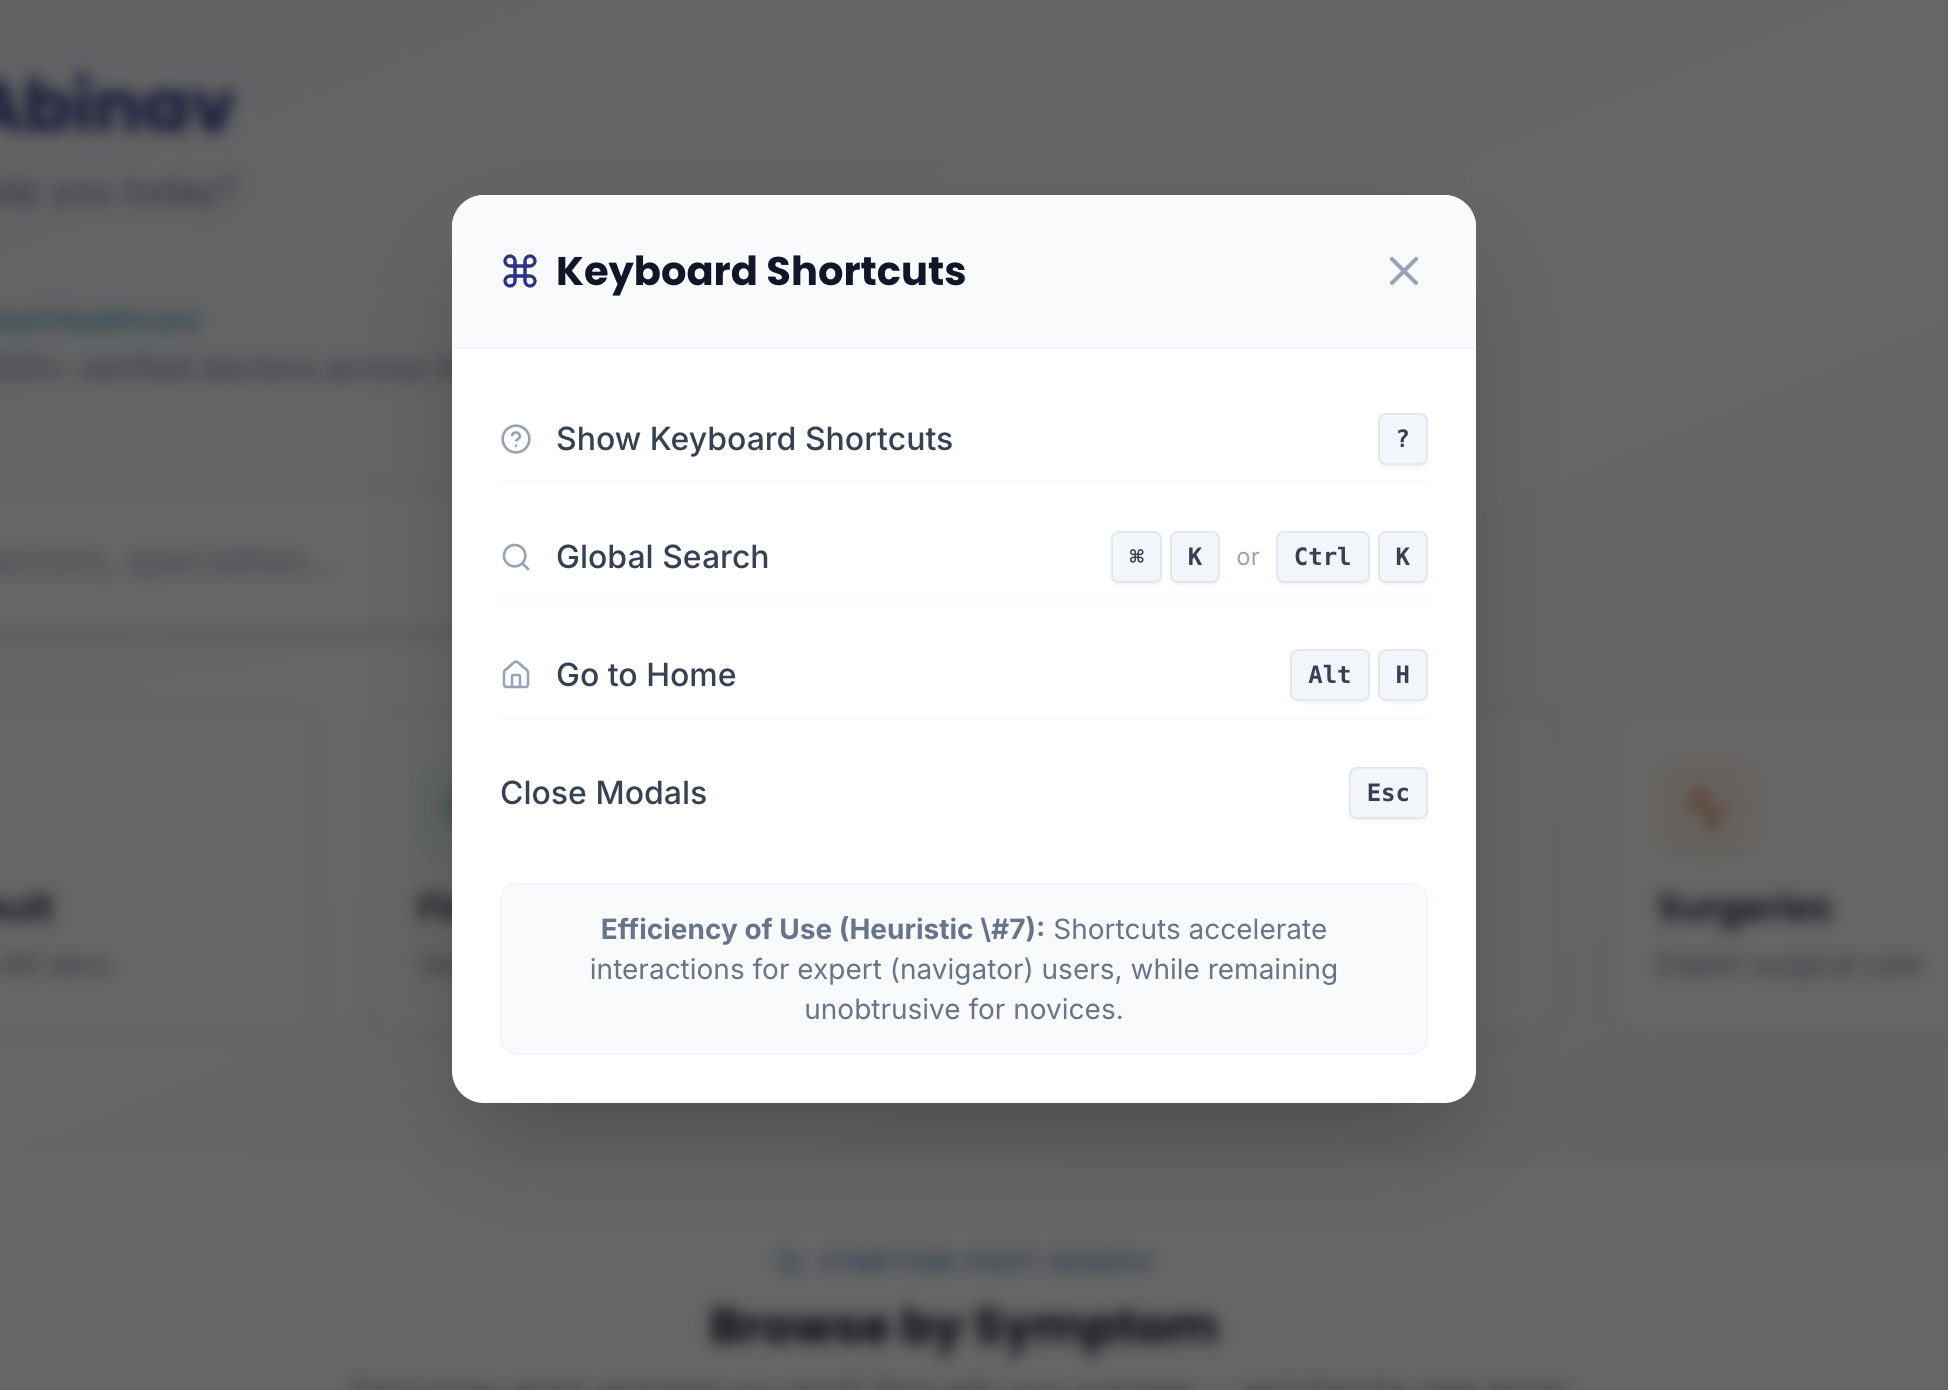
\includegraphics[width=0.6\textwidth]{keyboard_shortcuts_modal.png}}
    \caption{The Keyboard Shortcuts visual helper modal triggered by the \texttt{?} key, demonstrating Heuristic \#7 (Efficiency of Use). \textit{Phase 7.5 implementation.}}
\end{figure}

\vspace{0.5cm}

% =================================================================
\section{Block I --- Universal Design (7 Principles)}
% =================================================================

\begin{hcibox}{Universal Design --- 7 Principles (Mace et al., 1997)}
Universal Design creates products usable by all people, to the greatest extent possible, without adaptation. The 7 principles: \textbf{Equitable Use}, \textbf{Flexibility in Use}, \textbf{Simple \& Intuitive}, \textbf{Perceptible Information}, \textbf{Tolerance for Error}, \textbf{Low Physical Effort}, and \textbf{Size \& Space for Approach and Use}.

\textit{Reference: End-Sem HCI Lecture Notes, lines 428--617.}
\end{hcibox}

\subsection{I1 --- Equitable Use: ARIA Labels on All Interactive Elements}

\begin{featurebox}{Equitable Use --- Screen Reader Accessibility}
Universal Design Principle 1 (Equitable Use): ``provide the same means of use for all users.'' For keyboard and screen-reader users, interactive elements without labels are invisible. In BetterPracto:
\begin{itemize}[leftmargin=1.5em, itemsep=0pt]
  \item \texttt{Navbar.jsx} --- \texttt{aria-label="Primary navigation"} on \texttt{<nav>}, \texttt{aria-label="Toggle mobile menu"} on hamburger, \texttt{aria-expanded} dynamically set.
  \item \texttt{Search.jsx} --- \texttt{aria-label} on filter pills and sort pills (not just icon buttons).
  \item \texttt{ChatbotAssistant.jsx} --- \texttt{aria-label="Open chat assistant"}, \texttt{role="dialog"}, \texttt{aria-live="polite"} on bot messages, \texttt{aria-label="Chat message"} on input, \texttt{aria-label="Send message"} on button.
  \item \texttt{Help.jsx} --- \texttt{aria-expanded} on accordion FAQ buttons (announces open/closed state).
\end{itemize}
\end{featurebox}

\subsection{I2 --- Tolerance for Error: Booking Review Step}

\begin{featurebox}{Tolerance for Error --- Review Before Confirm}
Universal Design Principle 5 (Tolerance for Error): ``minimize hazards and the adverse consequences of accidental or unintended actions.'' The Booking flow enforces a 3-step flow --- Select Slot $\to$ Fill Details $\to$ Confirm --- where Step 2 shows all entered information before submission, giving the user an opportunity to review and correct before the irreversible ``Confirm Booking'' action. This mirrors Gmail's ``Undo Send'' pattern: a pre-commit checkpoint, not a post-error recovery.
\end{featurebox}

\begin{figure}[H]
    \centering
    \imgborder{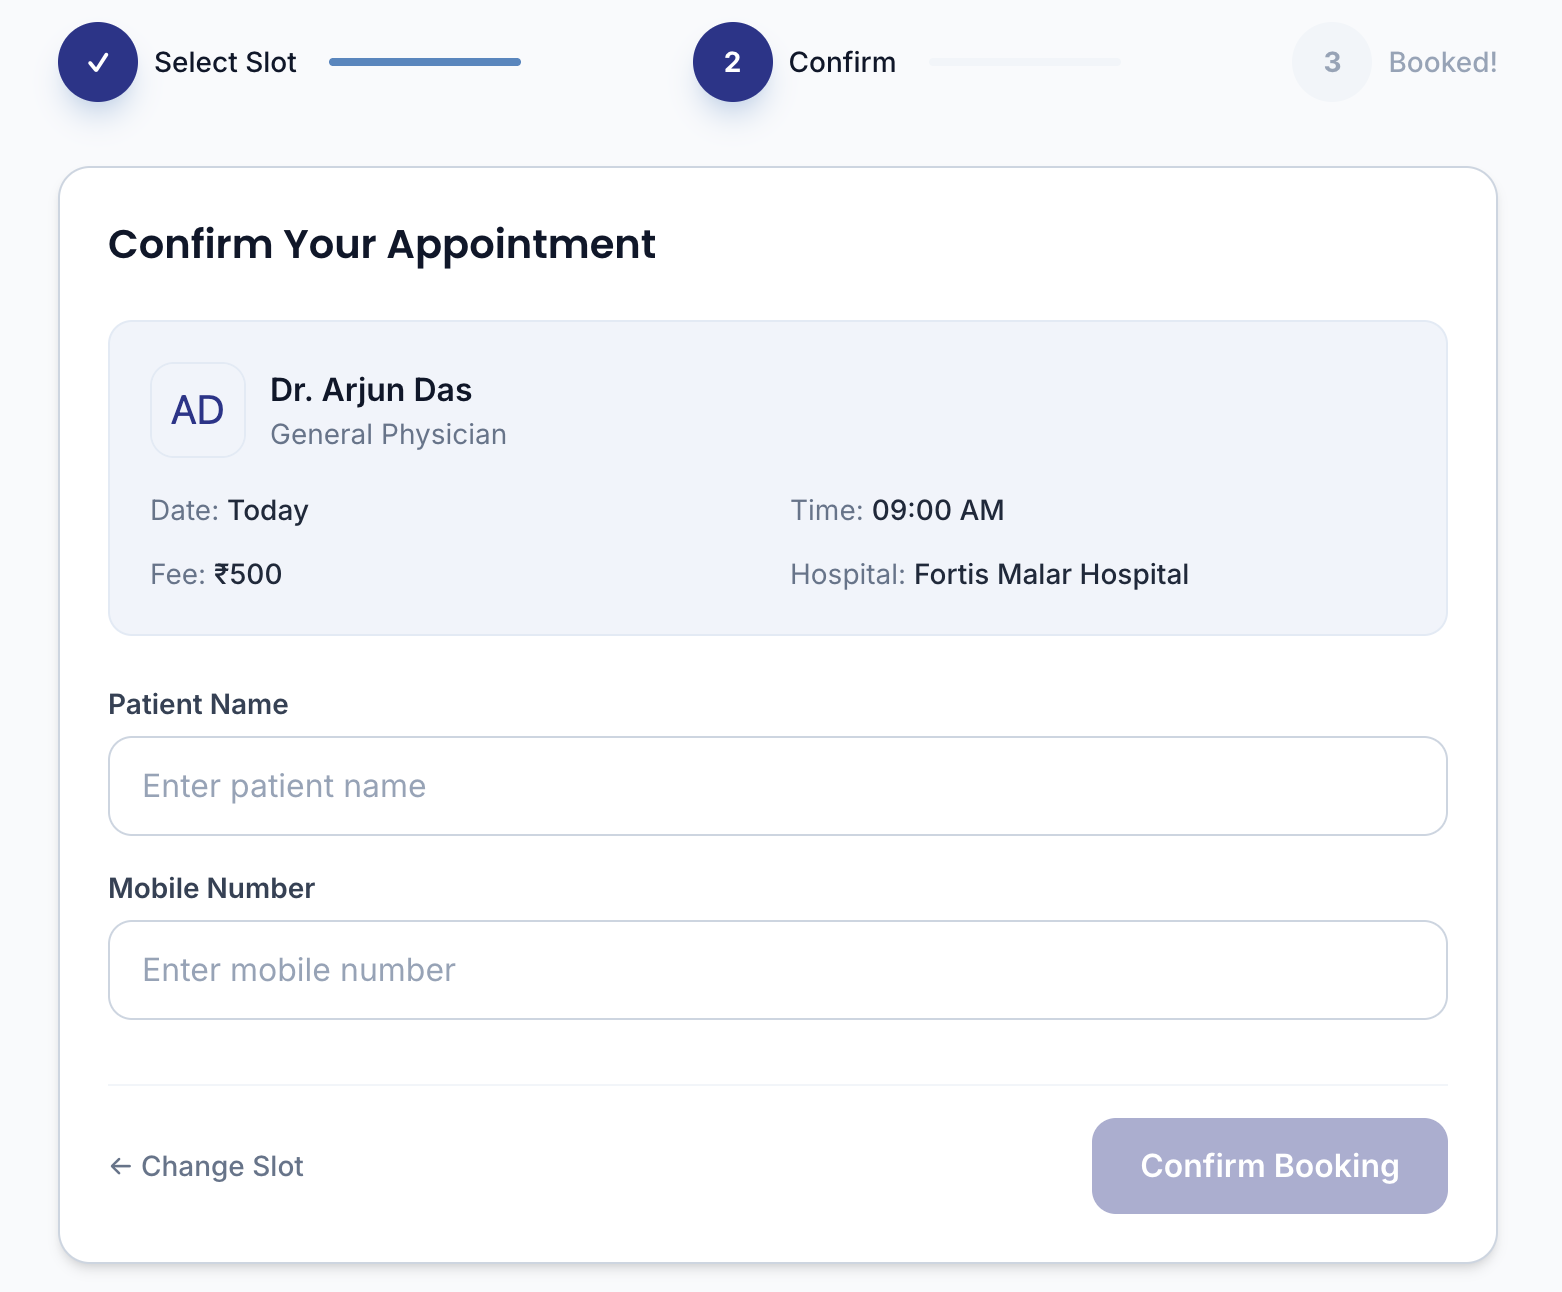
\includegraphics[width=0.8\textwidth]{universal_design_tolerance_error.png}}
    \caption{Tolerance for Error (Block I): Step 2 of the booking flow acts as a confirmation checkpoint, forcing a review of details before committing the data.}
\end{figure}

\subsection{I3 --- Size \& Space for Approach and Use: Touch Targets}

\begin{featurebox}{Touch Target Sizing --- Universal Design Principle 7}
Universal Design Principle 7 (Size and Space): ``provide adequate size for touch targets regardless of the user's body size or dexterity.'' WCAG 2.5.5 recommends a minimum touch target of 44$\times$44px. In BetterPracto, time slot buttons on the Booking page use \texttt{min-h-[44px] py-3}, ensuring they meet this threshold. Small slot buttons are a known pain point on mobile health apps --- insufficient target size causes mis-taps, leading to incorrect appointment times being selected.
\end{featurebox}

\subsection{I4 --- Flexibility in Use: OTP Alternative Login}

\begin{featurebox}{Flexibility in Use --- Multimodal Authentication}
Universal Design Principle 2 (Flexibility in Use): ``accommodate a wide range of individual preferences and abilities.'' By offering both traditional Email/Password login and a Phone/OTP (One-Time Password) alternative, the system provides choice in methods of use. The OTP login flow also supports international users via a country code dropdown, and incorporates Tolerance for Error by validating the phone number before firing the SMS logic.
\end{featurebox}

\begin{figure}[H]
    \centering
    \begin{subfigure}[b]{0.32\textwidth}
        \imgborder{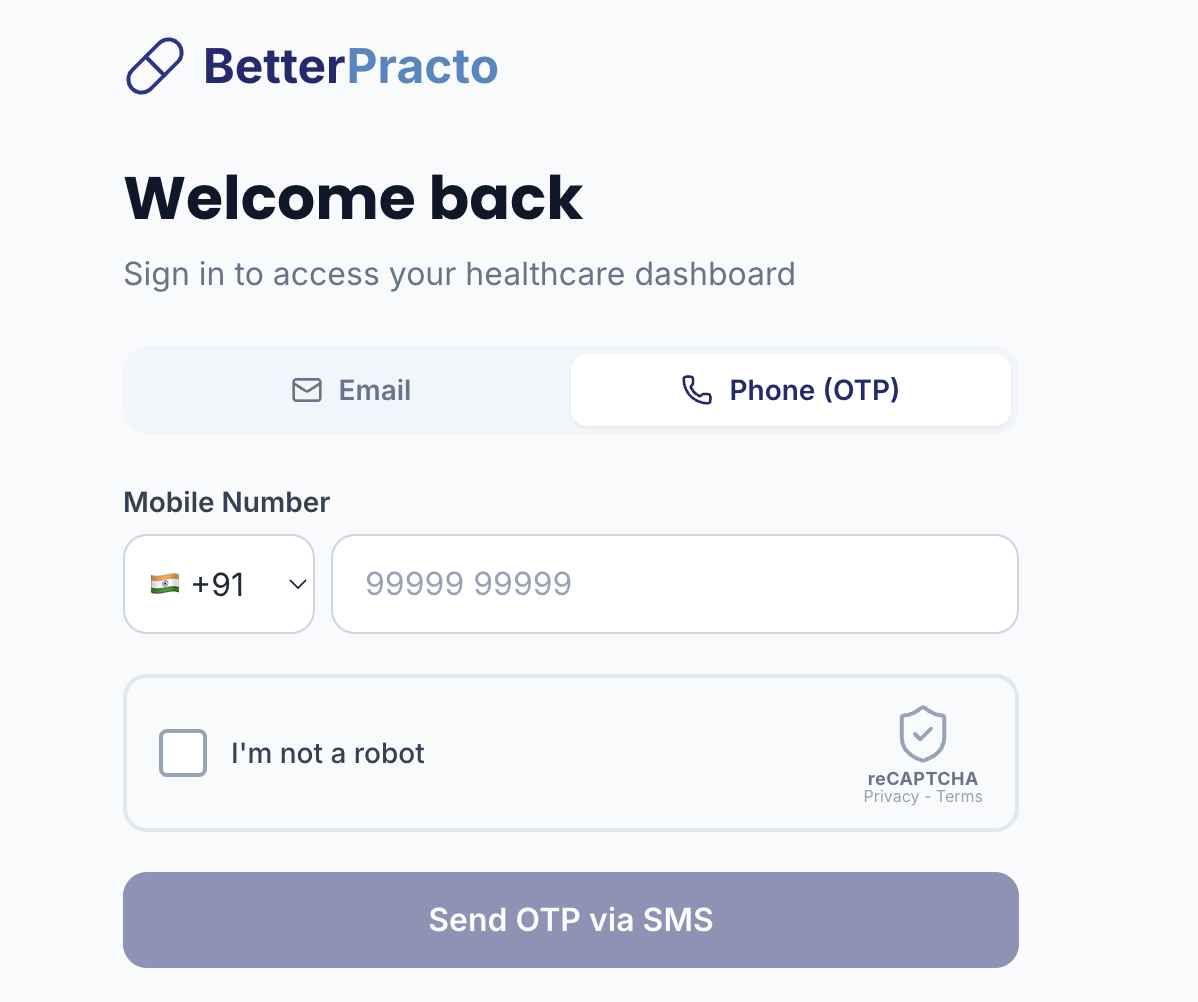
\includegraphics[width=\textwidth]{otp_login.png}}
        \caption{Phone login mode with country code selector.}
    \end{subfigure}
    \hfill
    \begin{subfigure}[b]{0.32\textwidth}
        \imgborder{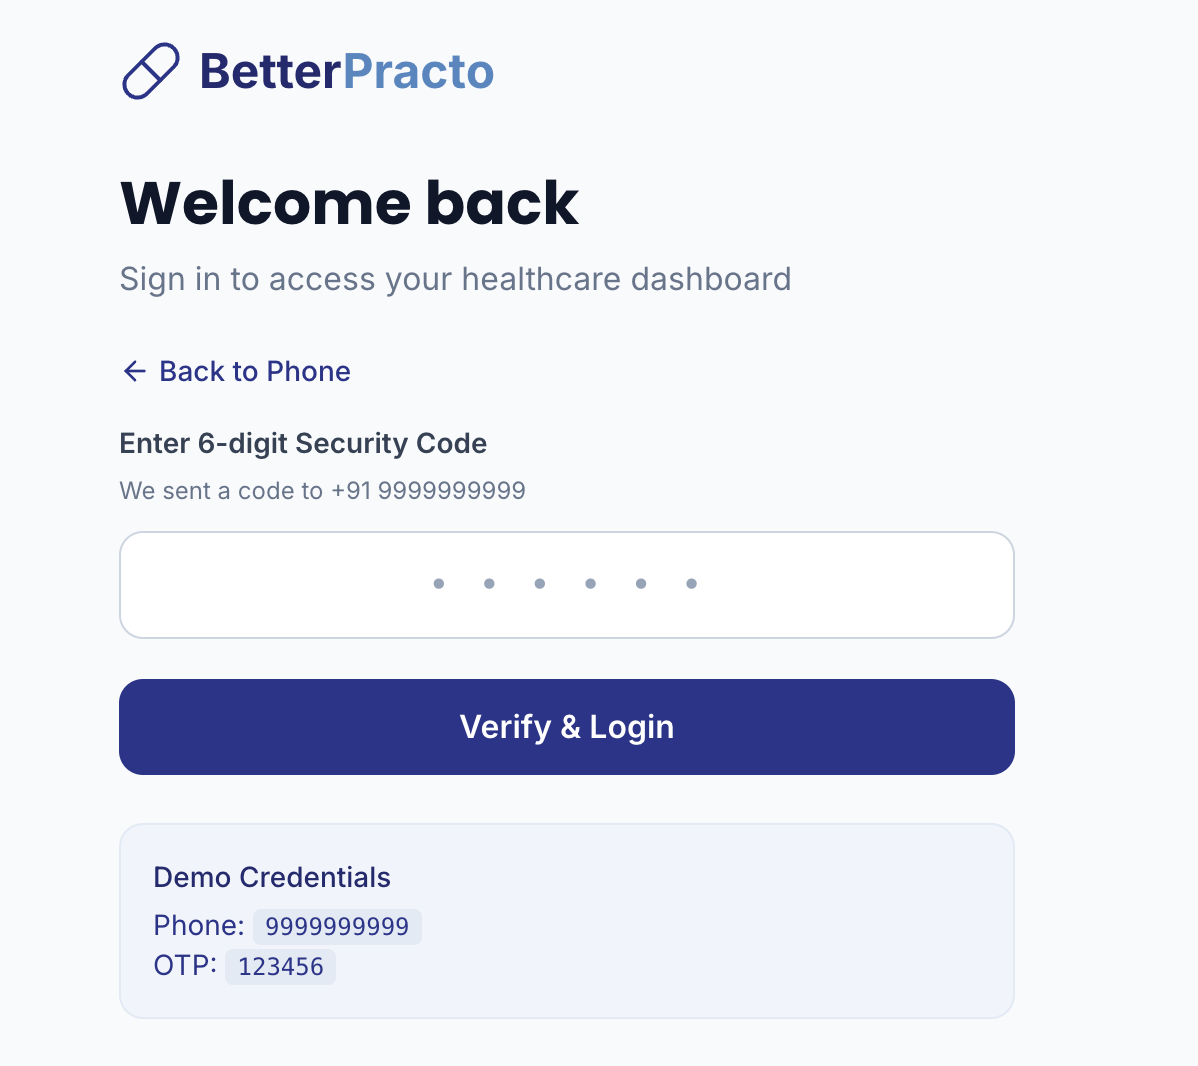
\includegraphics[width=\textwidth]{otp_login_sms_1.png}}
        \caption{Validation error on invalid phone format.}
    \end{subfigure}
    \hfill
    \begin{subfigure}[b]{0.32\textwidth}
        \imgborder{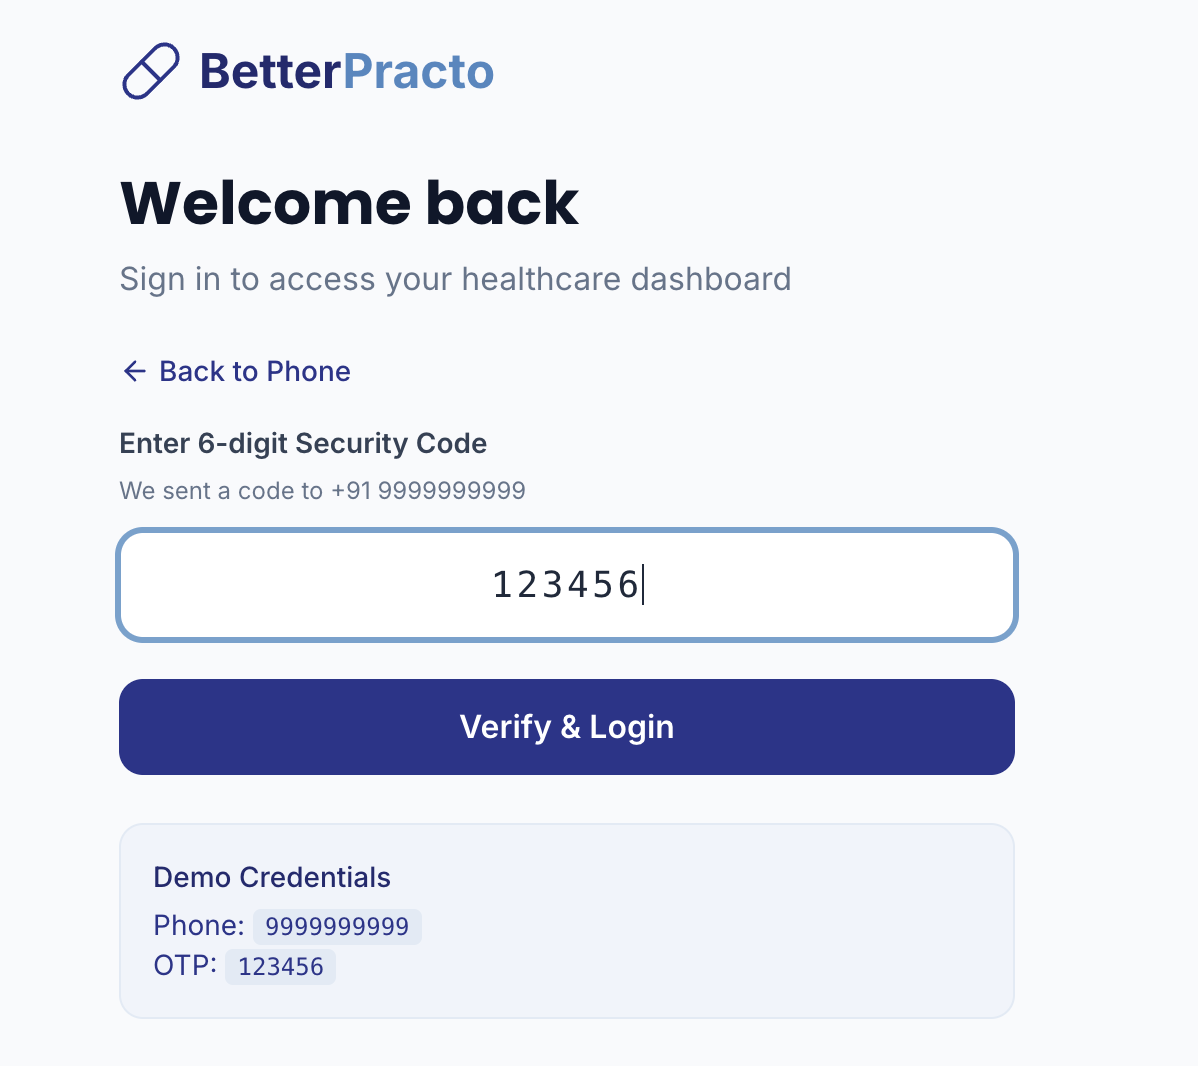
\includegraphics[width=\textwidth]{otp_login_sms_2.png}}
        \caption{OTP verification screen indicating code sent.}
    \end{subfigure}
    \caption{The OTP login flow demonstrating Flexibility in Use (Universal Design). \textit{Phase 7.5 implementation.}}
\end{figure}

\vspace{0.5cm}


% =================================================================
\section{Block K --- CAPTCHA Design Principles}
% =================================================================

\begin{hcibox}{CAPTCHA Design Principles}
CAPTCHA (Completely Automated Public Turing test to tell Computers and Humans Apart) must balance \textbf{security} (block bots) with \textbf{accessibility} (usable by humans with disabilities). Text-distortion CAPTCHAs violate Universal Design Principle 1 (Equitable Use) because they are inaccessible to visually impaired users. The evolution: distorted text $\to$ image recognition $\to$ reCAPTCHA v2 (checkbox + risk analysis) $\to$ reCAPTCHA v3 (invisible, score-based).

\textit{Reference: End-Sem HCI Lecture Notes, lines 626--746.}
\end{hcibox}

\subsection{K1 --- reCAPTCHA v2 Implementation}

\begin{featurebox}{reCAPTCHA ``I'm not a robot'' Checkbox (Block K)}
Based on the end-semester reference on CAPTCHA evolution, reCAPTCHA v2 is implemented on the Login page as the optimal balance of security and accessibility. The traditional distorted-text (Gimpy) CAPTCHAs create high cognitive load and violate Universal Design Principle 1 (Equitable Use) for elderly or visually impaired users.

The reCAPTCHA v2 checkbox requires zero visual puzzle-solving. The risk-engine invisibly analyses mouse movement patterns and timings.

\textbf{HCI \& Usability aspects implemented:}
\begin{itemize}[leftmargin=1.5em, itemsep=0pt]
  \item \textbf{Tolerance for Error:} The ``Sign In'' button remains disabled (\texttt{disabled=true}) until the CAPTCHA is verified, preventing premature submission errors.
  \item \textbf{Informative Feedback:} Clicking the checkbox transitions it from empty $\to$ loading spinner (simulating risk-engine evaluation) $\to$ green checkmark (verified label).
  \item \textbf{Learnability / Flexibility:} A ``Reset verification'' button appears after verification, an accessibility requirement allowing the user to regenerate the challenge if needed.
  \item \textbf{Authority \& Trust:} The inclusion of the recognisable reCAPTCHA branding (shield logo and wordmark) triggers the Persuasion principle of Authority, increasing user trust in the platform's security.
\end{itemize}
\end{featurebox}

\begin{figure}[H]
    \centering
    \begin{subfigure}[b]{0.47\textwidth}
        \imgborder{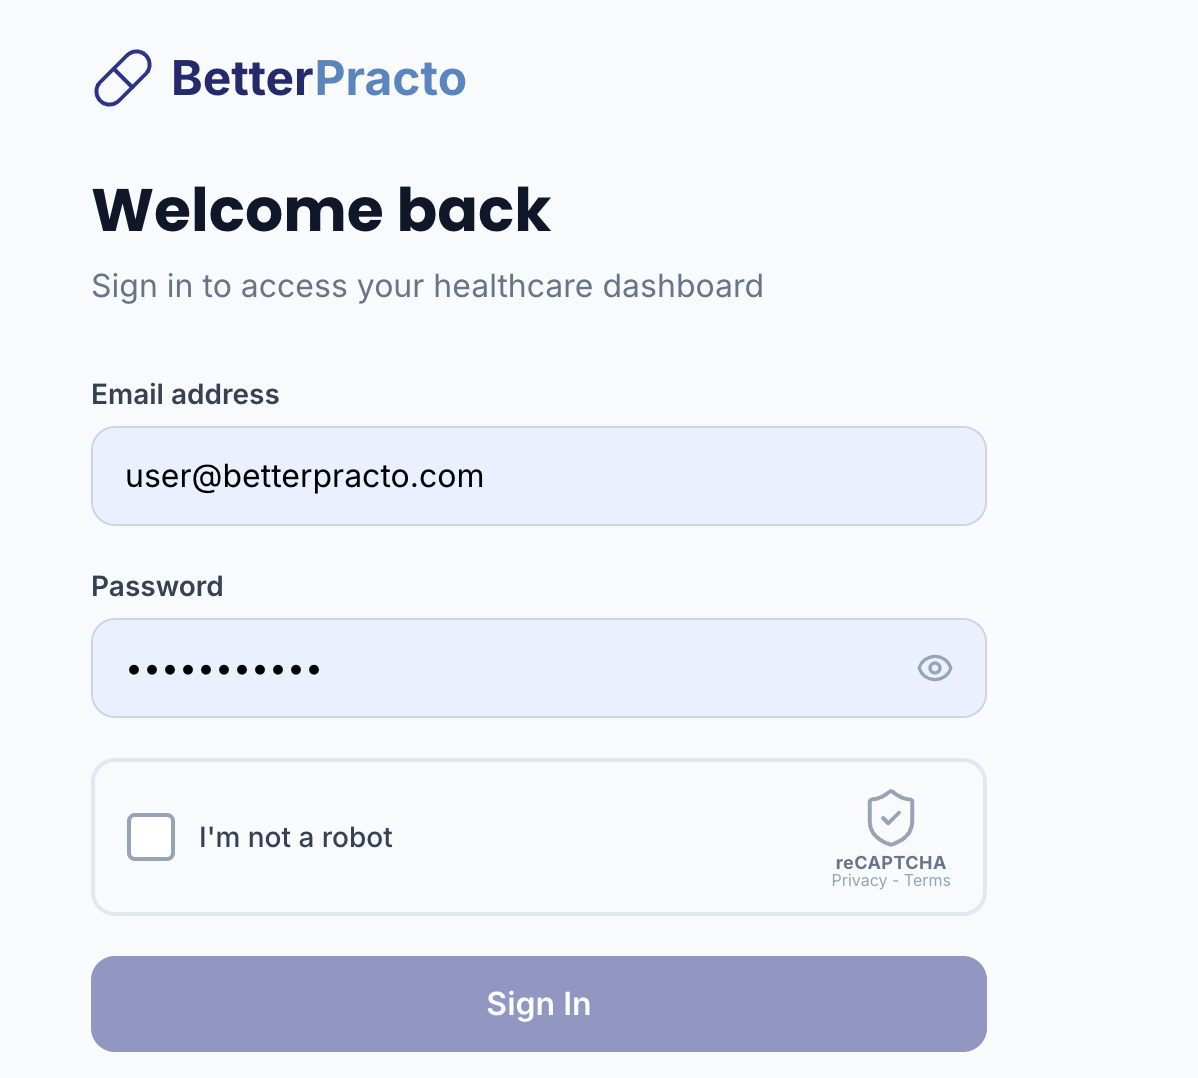
\includegraphics[width=\textwidth]{captcha_login.png}}
        \caption{Unverified CAPTCHA. The ``Sign In'' button is locked. \textit{Block K.}}
    \end{subfigure}
    \hfill
    \begin{subfigure}[b]{0.47\textwidth}
        \imgborder{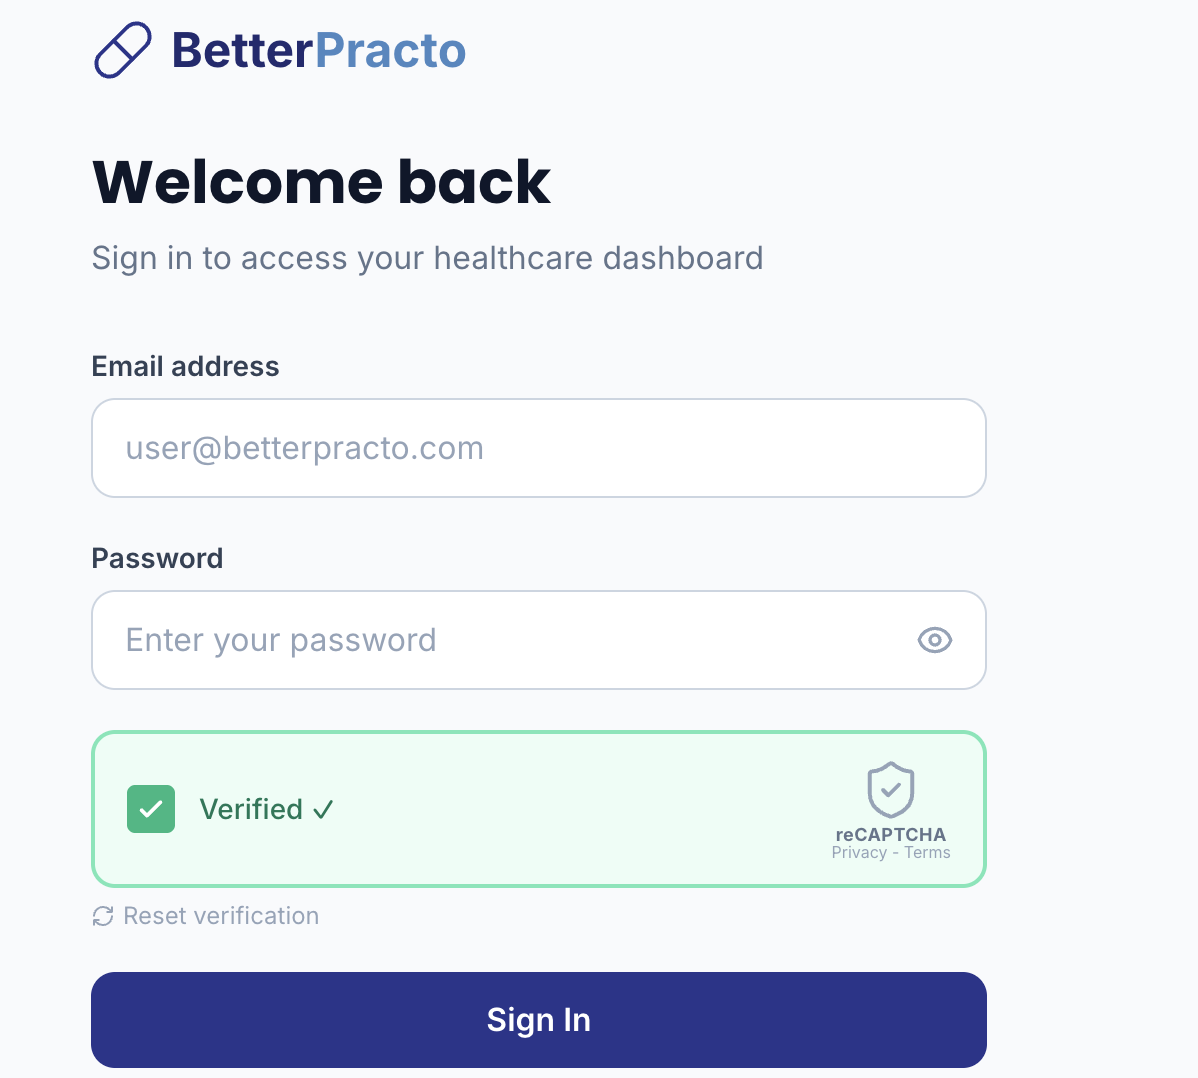
\includegraphics[width=\textwidth]{captcha_solved.png}}
        \caption{Verified CAPTCHA. The risk-engine shows a green checkmark and unlocks the sign in process. \textit{Block K.}}
    \end{subfigure}
    \caption{The Login page featuring the ``I'm not a robot'' reCAPTCHA v2 widget simulated UI. The button remains locked until verification is complete.}
\end{figure}

\vspace{0.5cm}

% =================================================================
\section{Enhanced Mid-Sem Features}
% =================================================================

\begin{hcibox}{Enhanced Mid-Sem Features}
The end-semester implementation enhances the following mid-semester violations with new HCI concepts not available at mid-sem:
\begin{itemize}[leftmargin=1.5em, itemsep=0pt]
  \item \textbf{V3 (Doctor Cards)} --- Added framer-motion \texttt{AnimatePresence} layout animation to the sort interaction --- Direct Manipulation + Common Fate (Gestalt).
  \item \textbf{V4 (Onboarding)} --- Added 4th step ``Help is Always Here'' introducing the User Support Systems (Block E) concept.
  \item \textbf{V6 (Help Page)} --- Added Quick Reference card at the top --- User Support Systems, Quick Reference type.
  \item \textbf{V8 (Active Nav)} --- Added skip navigation link, keyboard focus indicators, ARIA labels --- Universal Design (Block I).
  \item \textbf{V12 (Sort)} --- Sort animation now demonstrates Common Fate (Gestalt) + Direct Manipulation simultaneously.
\end{itemize}
\end{hcibox}

\subsection{L1 --- V4 Enhancement: Onboarding User Support Integration}

\begin{figure}[H]
    \centering
    \imgborder{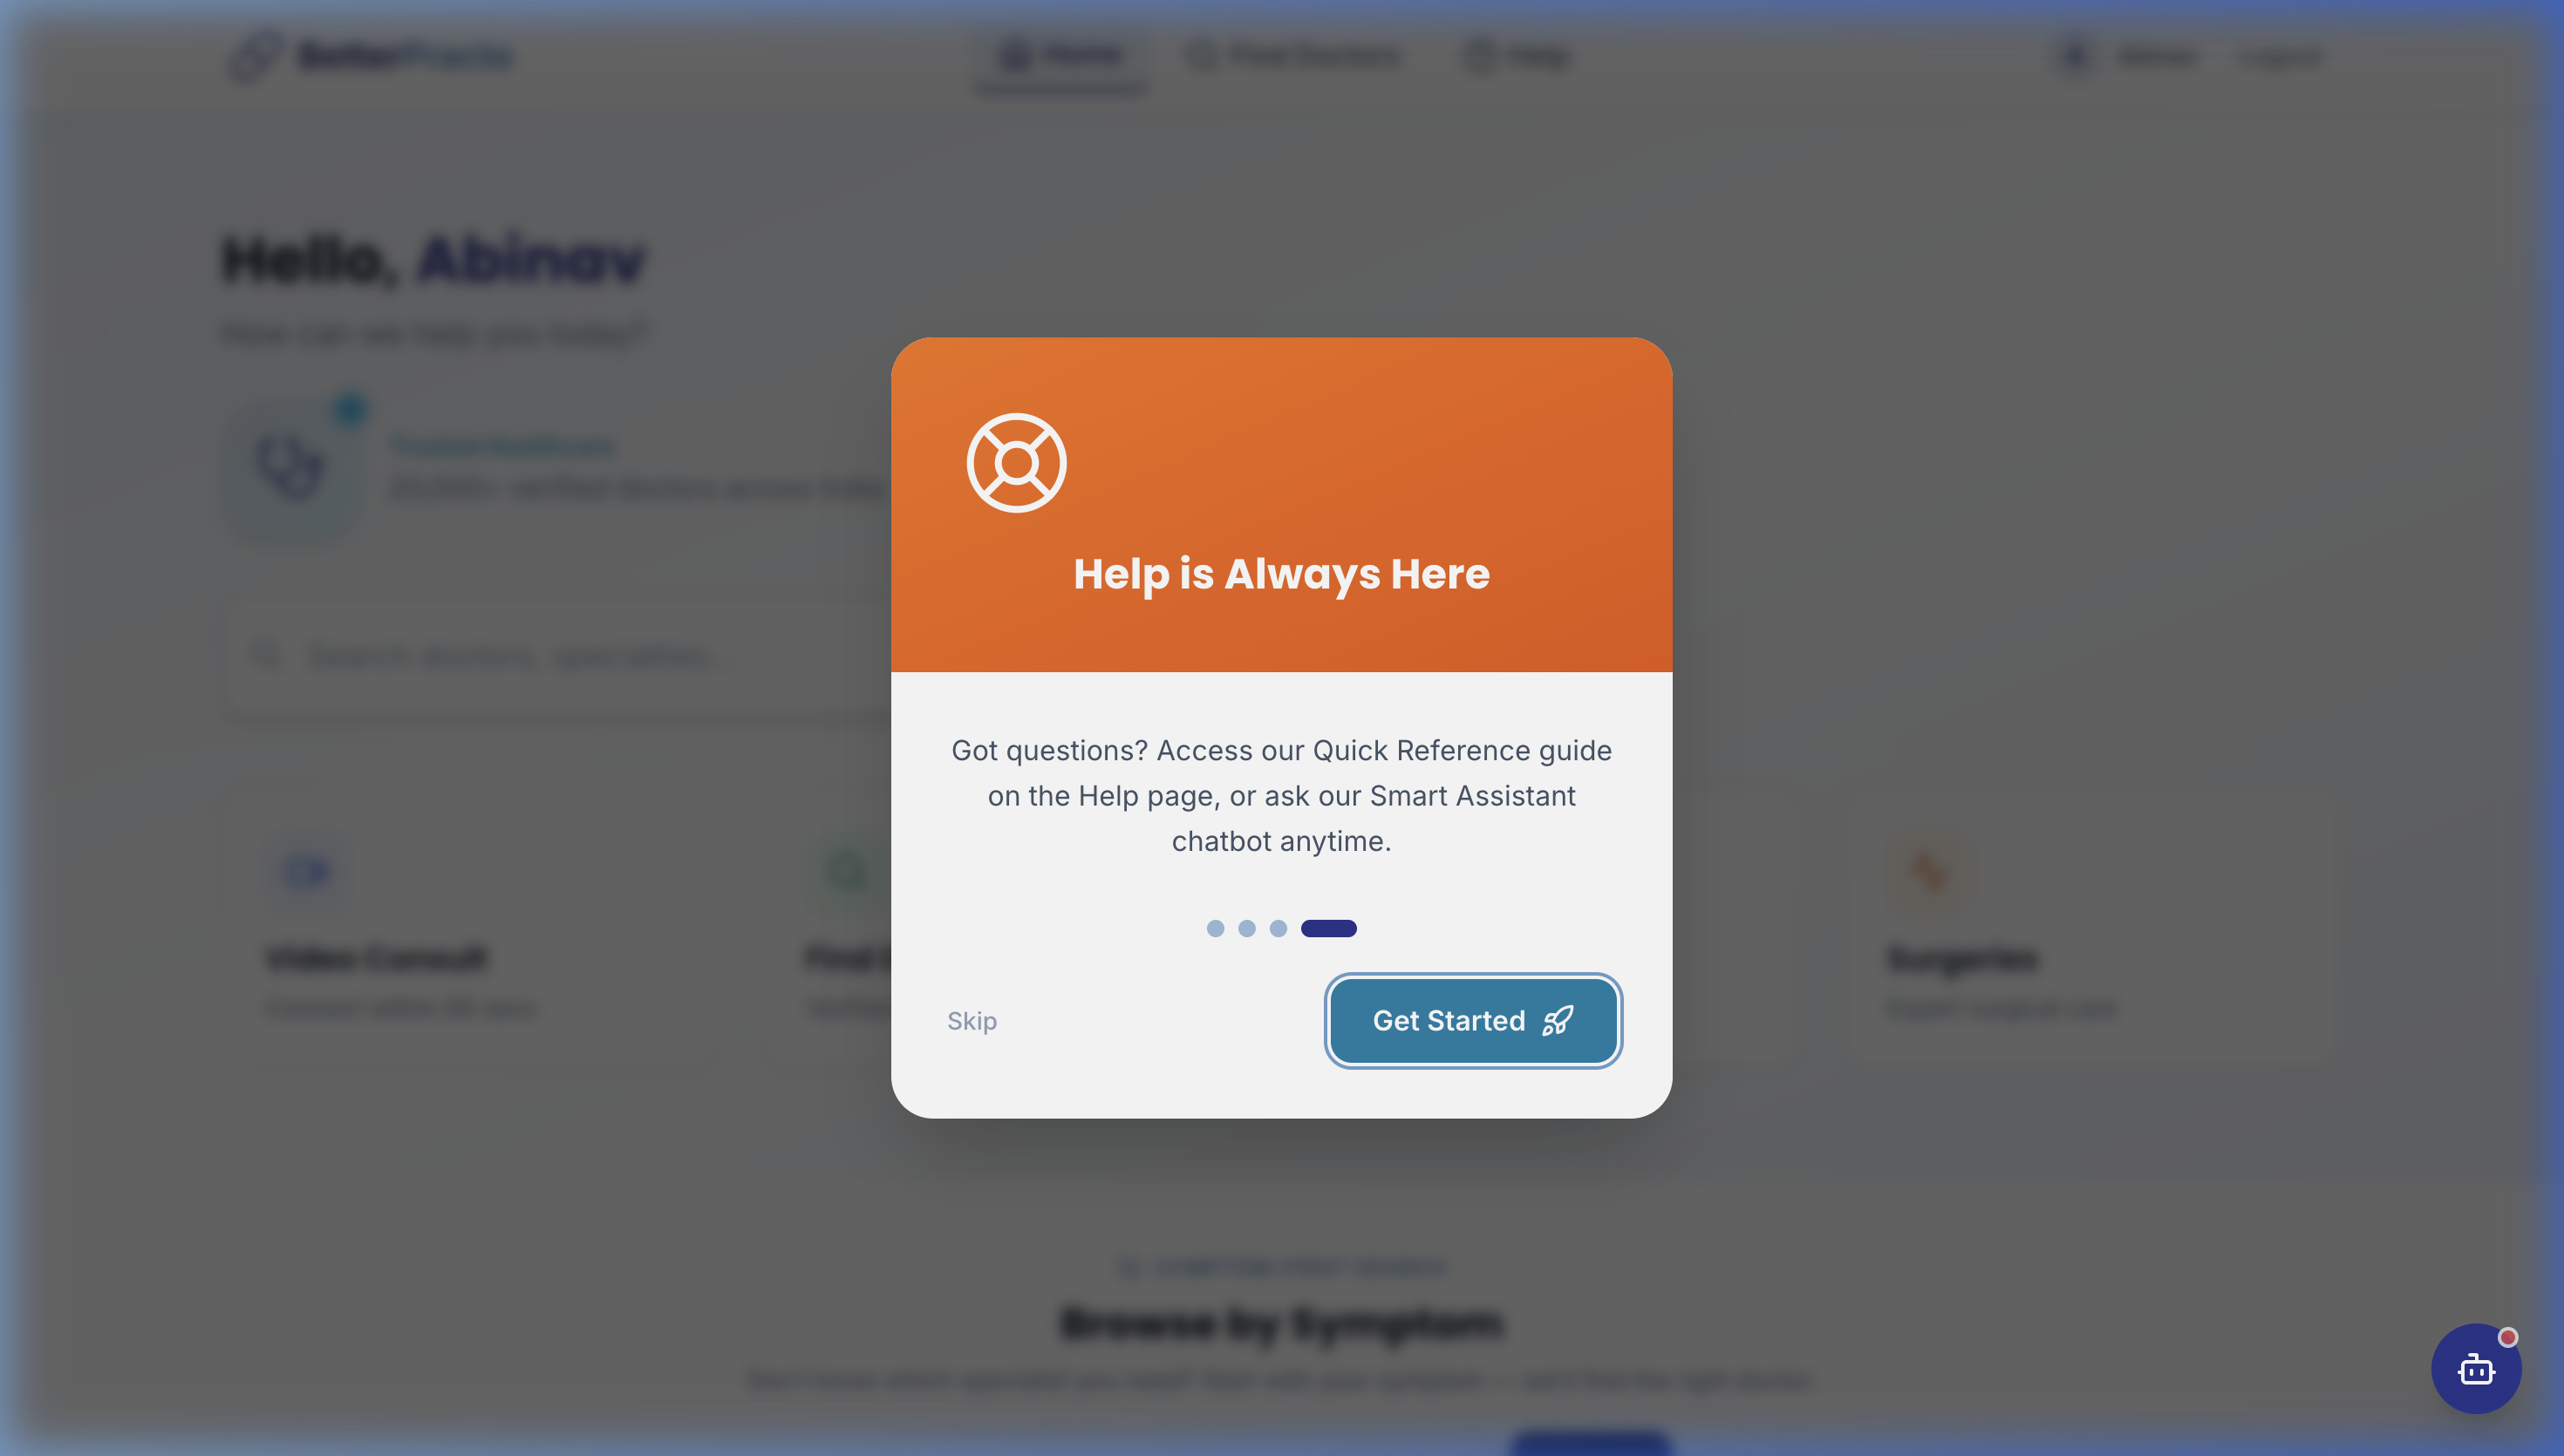
\includegraphics[width=0.6\textwidth]{enhanced_v4_onboarding4.png}}
    \caption{The enhanced V4 Onboarding flow now includes a 4th step explicitly introducing the User Support systems (Quick Reference and Assistant), applying the Learnability principle by orienting new users to available help channels before they start using the app. \textit{Block L.}}
\end{figure}

\subsection{L2 --- V6 Enhancement: Quick Reference Card}

\begin{figure}[H]
    \centering
    \imgborder{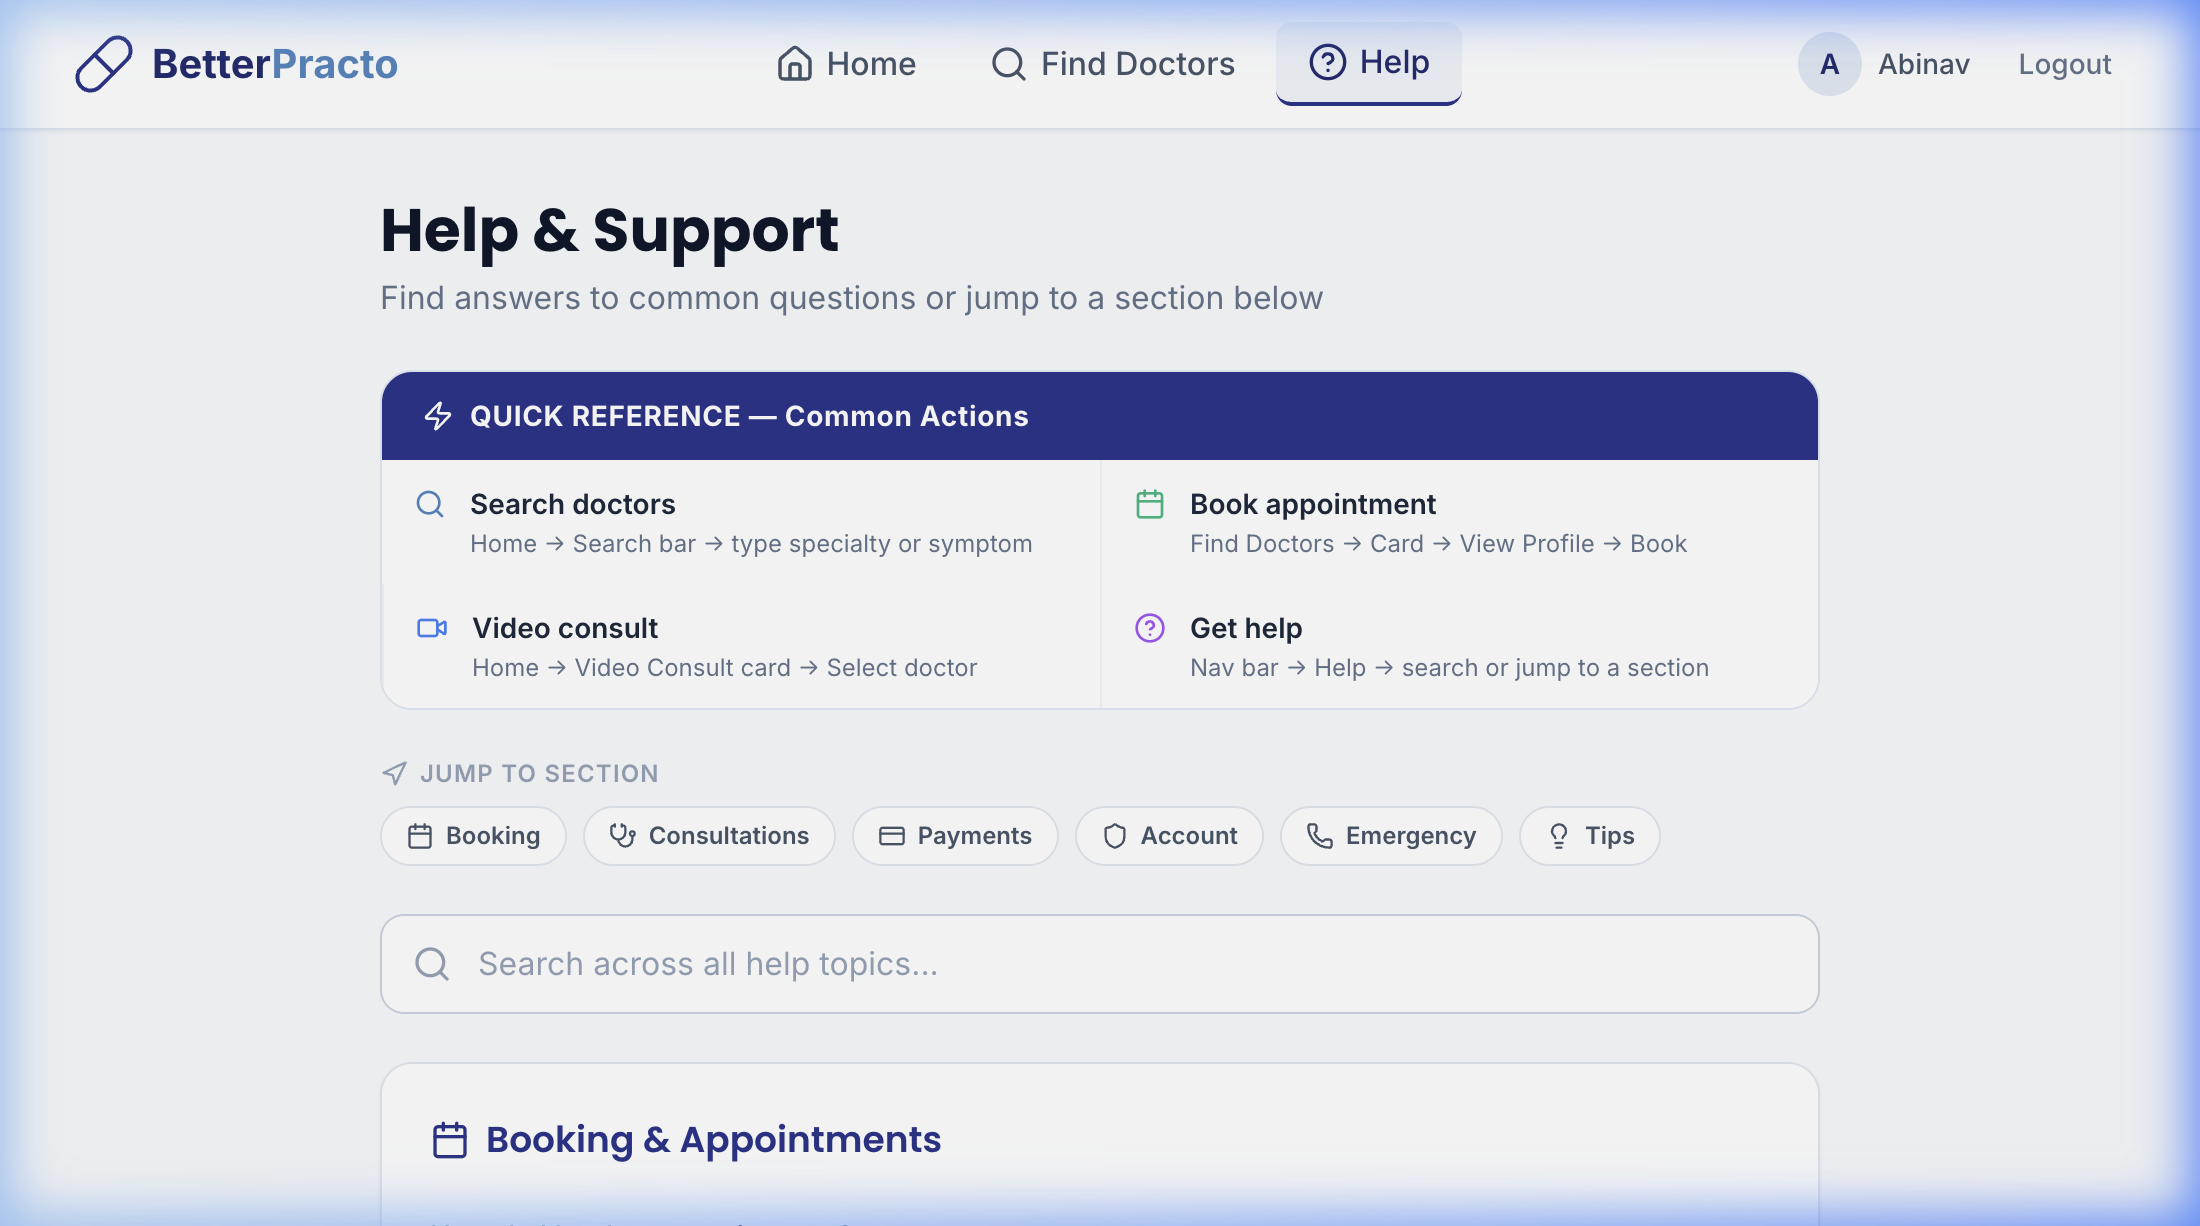
\includegraphics[width=0.8\textwidth]{user_support_quickref.png}}
    \caption{The Help page enhanced from V6 now includes a prominent Quick Reference card, addressing the User Support system requirements for providing immediate, rule-based reminders to users. \textit{Block L \& Block E.}}
\end{figure}

\vspace{0.5cm}

% =================================================================
\section{Complete HCI Concept Coverage Table}
% =================================================================

\begin{center}
\begin{longtable}{>{\bfseries}p{3.5cm} p{4cm} p{5cm}}
\toprule
\textbf{HCI Concept} & \textbf{Feature} & \textbf{Where in App} \\
\midrule
\endfirsthead
\multicolumn{3}{c}{\textit{(continued)}} \\
\toprule
\textbf{HCI Concept} & \textbf{Feature} & \textbf{Where in App} \\
\midrule
\endhead
Gestalt Proximity & Name/specialty group vs availability group & Search page --- card layout \\
Gestalt Similarity & Identical Verified badge \& availability pill styles & Search page --- all cards \\
Gestalt Figure \& Ground & White cards on grey background & Search page \\
Gestalt Continuity & Left-border stripe on card metadata & Search page --- card left edge \\
Gestalt Common Fate & framer-motion sort animation & Search page --- sort pills \\
Gestalt Closure & Step progress indicator circles & Booking page \\
Visual Dominance & Hero stethoscope icon on home & Home page --- hero section \\
Visual Scale & Search bar larger than other inputs & Home page --- search bar \\
Visual Balance & Equal-width 4-card hero grid & Home page --- quick actions \\
Visual Hierarchy & 3-level typography (name/specialty/meta) & Doctor Profile page \\
Visual Negative Space & Section padding, breathing room & All pages \\
Persuasion: Social Proof & ``X people viewed today'' badge & Doctor Profile page \\
Persuasion: Scarcity & ``Only N slots left!'' badge & Booking Step 1 \\
Persuasion: Authority & Awards \& Recognition section & Doctor Profile page \\
Persuasion: Reciprocity & ``Free 1st Consult'' badge & Home page / Doctor cards \\
Persuasion: Commitment & Health reminders checkbox & Booking Step 3 (success) \\
Color Psychology & Trust blue / health green / warning amber & Global --- all pages \\
Shape Psychology & rounded-xl buttons / rounded-full pills & Global --- all pages \\
Quick Reference & Cheat sheet at top of Help page & Help page \\
Task-Specific Help & ContextHelpTooltip on form fields & Booking Step 2 fields \\
Tutorial & 4-step onboarding (incl. Help step) & Home --- on first login \\
Non-intrusive Assistant & AssistantBubble on Booking page & Booking page --- bottom-right \\
Navigation: Skip Link & \texttt{Skip to main content} link & Navbar --- keyboard focus \\
Navigation: Breadcrumb & Reusable Breadcrumb component & Doctor Profile + Booking \\
Navigation: Keyboard & Logo keyboard navigable + ARIA labels & Navbar \\
Menu Selection & Specialty filter pills & Search page \\
Direct Manipulation & Sort animation + slot tap feedback & Search + Booking Step 1 \\
Form Fill-in & Patient details form & Booking Step 2 \\
Web Usability: 404 & Custom NotFound page & Any invalid URL \\
Web Usability: SEO & OG + Twitter meta tags & index.html \\
Feature Exposure & ``Browse by Symptom'' section & Home page \\
Universal: Equitable Use & ARIA labels on all icon buttons & Navbar, Search \\
Universal: Percept. Info & Text + colour on availability badges & Search cards \\
Universal: Tolerance Error & Review-before-confirm warning & Booking Step 2 \\
Universal: Low Effort & min-h-[44px] on touch targets & Booking Step 1 slots \\
Explorer Support & Symptom chips when query empty & Search page \\
Navigator Support & Recent searches via localStorage & Search page \\
CAPTCHA & ``I'm not a robot'' checkbox + UX rationale & Login page \\
\bottomrule
\end{longtable}
\end{center}

\vspace{0.5cm}

% =================================================================
\section{Summary}
% =================================================================

This end-semester extension of Better Practo demonstrates \textbf{12 distinct HCI concept blocks} covering the full post-mid-semester curriculum. Every feature was implemented in a live React prototype and documented with screenshots. Combined with the 14 violations fixed in the mid-semester, the final Better Practo prototype addresses \textbf{26 distinct HCI principles and case studies} across the entire CS5015 syllabus.

\begin{center}
\begin{tabular}{l c}
\toprule
\textbf{Metric} & \textbf{Count} \\
\midrule
Mid-sem violations fixed & 14 \\
End-sem concept blocks & 12 \\
Total HCI principles covered & 40+ \\
New React components created & 5 \\
Screenshots taken & 25+ \\
\bottomrule
\end{tabular}
\end{center}

\vspace{0.5cm}

% =================================================================
\section{Additional Links}
% =================================================================

\begin{itemize}[leftmargin=1.5em]
  \item \textbf{GitHub Repository:} \url{https://github.com/R-Abinav/hci-design-hackathon}
  \item \textbf{Original Practo:} \url{https://www.practo.com}
  \item \textbf{Mid-Sem Report:} See Part 2 of this PDF (appended below)
\end{itemize}

\vspace{1cm}

\hrule

\vspace{1cm}

\begin{center}
{\Huge\bfseries\color{midsemdark} --- END OF END-SEM REPORT ---}\\[0.4cm]
{\large The Mid-Semester Report follows on the next page.}
\end{center}

\vspace{1cm}

\hrule

\end{document}
